\documentclass[8pt,aspectratio=1610]{beamer}
\usepackage[utf8]{inputenc}
\usepackage{booktabs}
\usepackage{array}
\usepackage{graphicx}
\usepackage{xcolor}
\usepackage{tikz}
\usetikzlibrary{positioning,arrows.meta,decorations.pathreplacing,calc,shadows}
\usepackage{pgfplots}
\pgfplotsset{compat=1.18}
\usepackage{amsmath}
\usepackage{amssymb}
\usepackage{amsfonts}
\usepackage{algorithm}
\usepackage{algorithmic}

\usetheme{metropolis}
\usecolortheme{wolverine}
\metroset{progressbar=frametitle,block=fill}
\setbeamertemplate{navigation symbols}{}

% Define custom colors complementing the Wolverine theme
\definecolor{maizelight}{RGB}{255, 203, 5}
\definecolor{maizedark}{RGB}{255, 167, 0}
\definecolor{bluelight}{RGB}{0, 39, 76}
\definecolor{tealaccent}{RGB}{0, 128, 128}
\definecolor{orangeaccent}{RGB}{255, 138, 51}

% Customize block colors
\setbeamercolor{block title}{bg=bluelight,fg=white}
\setbeamercolor{block body}{bg=bluelight!10,fg=black}
\setbeamercolor{block title example}{bg=maizelight,fg=black}
\setbeamercolor{block body example}{bg=maizelight!15,fg=black}
\setbeamercolor{block title alerted}{bg=orangeaccent,fg=white}
\setbeamercolor{block body alerted}{bg=orangeaccent!15,fg=black}

% Custom block environments
\newenvironment<>{techblock}[1]{%
  \setbeamercolor{block title}{bg=tealaccent,fg=white}%
  \setbeamercolor{block body}{bg=tealaccent!10,fg=black}%
  \begin{block}#2{#1}}{\end{block}}

\newenvironment<>{tipblock}[1]{%
  \setbeamercolor{block title}{bg=maizedark,fg=black}%
  \setbeamercolor{block body}{bg=maizedark!15,fg=black}%
  \begin{block}#2{#1}}{\end{block}}

% Title slide information
\title{Principal Component Analysis}
\subtitle{CMSC 173 - Machine Learning}
\author{Noel Jeffrey Pinton}
\institute{Department of Computer Science\\University of the Philippines - Cebu}
\date{\today}

\begin{document}

\begin{frame}
\titlepage
\end{frame}

\begin{frame}{Outline}
\tableofcontents
\end{frame}

% ========================================
% Section: Introduction
% ========================================

\section{Introduction \& Motivation}

\begin{frame}{What is Principal Component Analysis?}
\begin{columns}[t]
\begin{column}{0.48\textwidth}
\begin{block}{Definition}
\textbf{Principal Component Analysis (PCA)} is a statistical technique that transforms high-dimensional data into a lower-dimensional representation while preserving as much variance as possible.
\end{block}

\vspace{0.2cm}

\begin{exampleblock}{Key Characteristics}
\begin{itemize}
\setlength{\itemsep}{2pt}
\item Unsupervised learning method
\item Linear dimensionality reduction
\item Orthogonal transformation
\item Variance maximization
\end{itemize}
\end{exampleblock}
\end{column}

\begin{column}{0.48\textwidth}
\centering
\vspace{0pt}
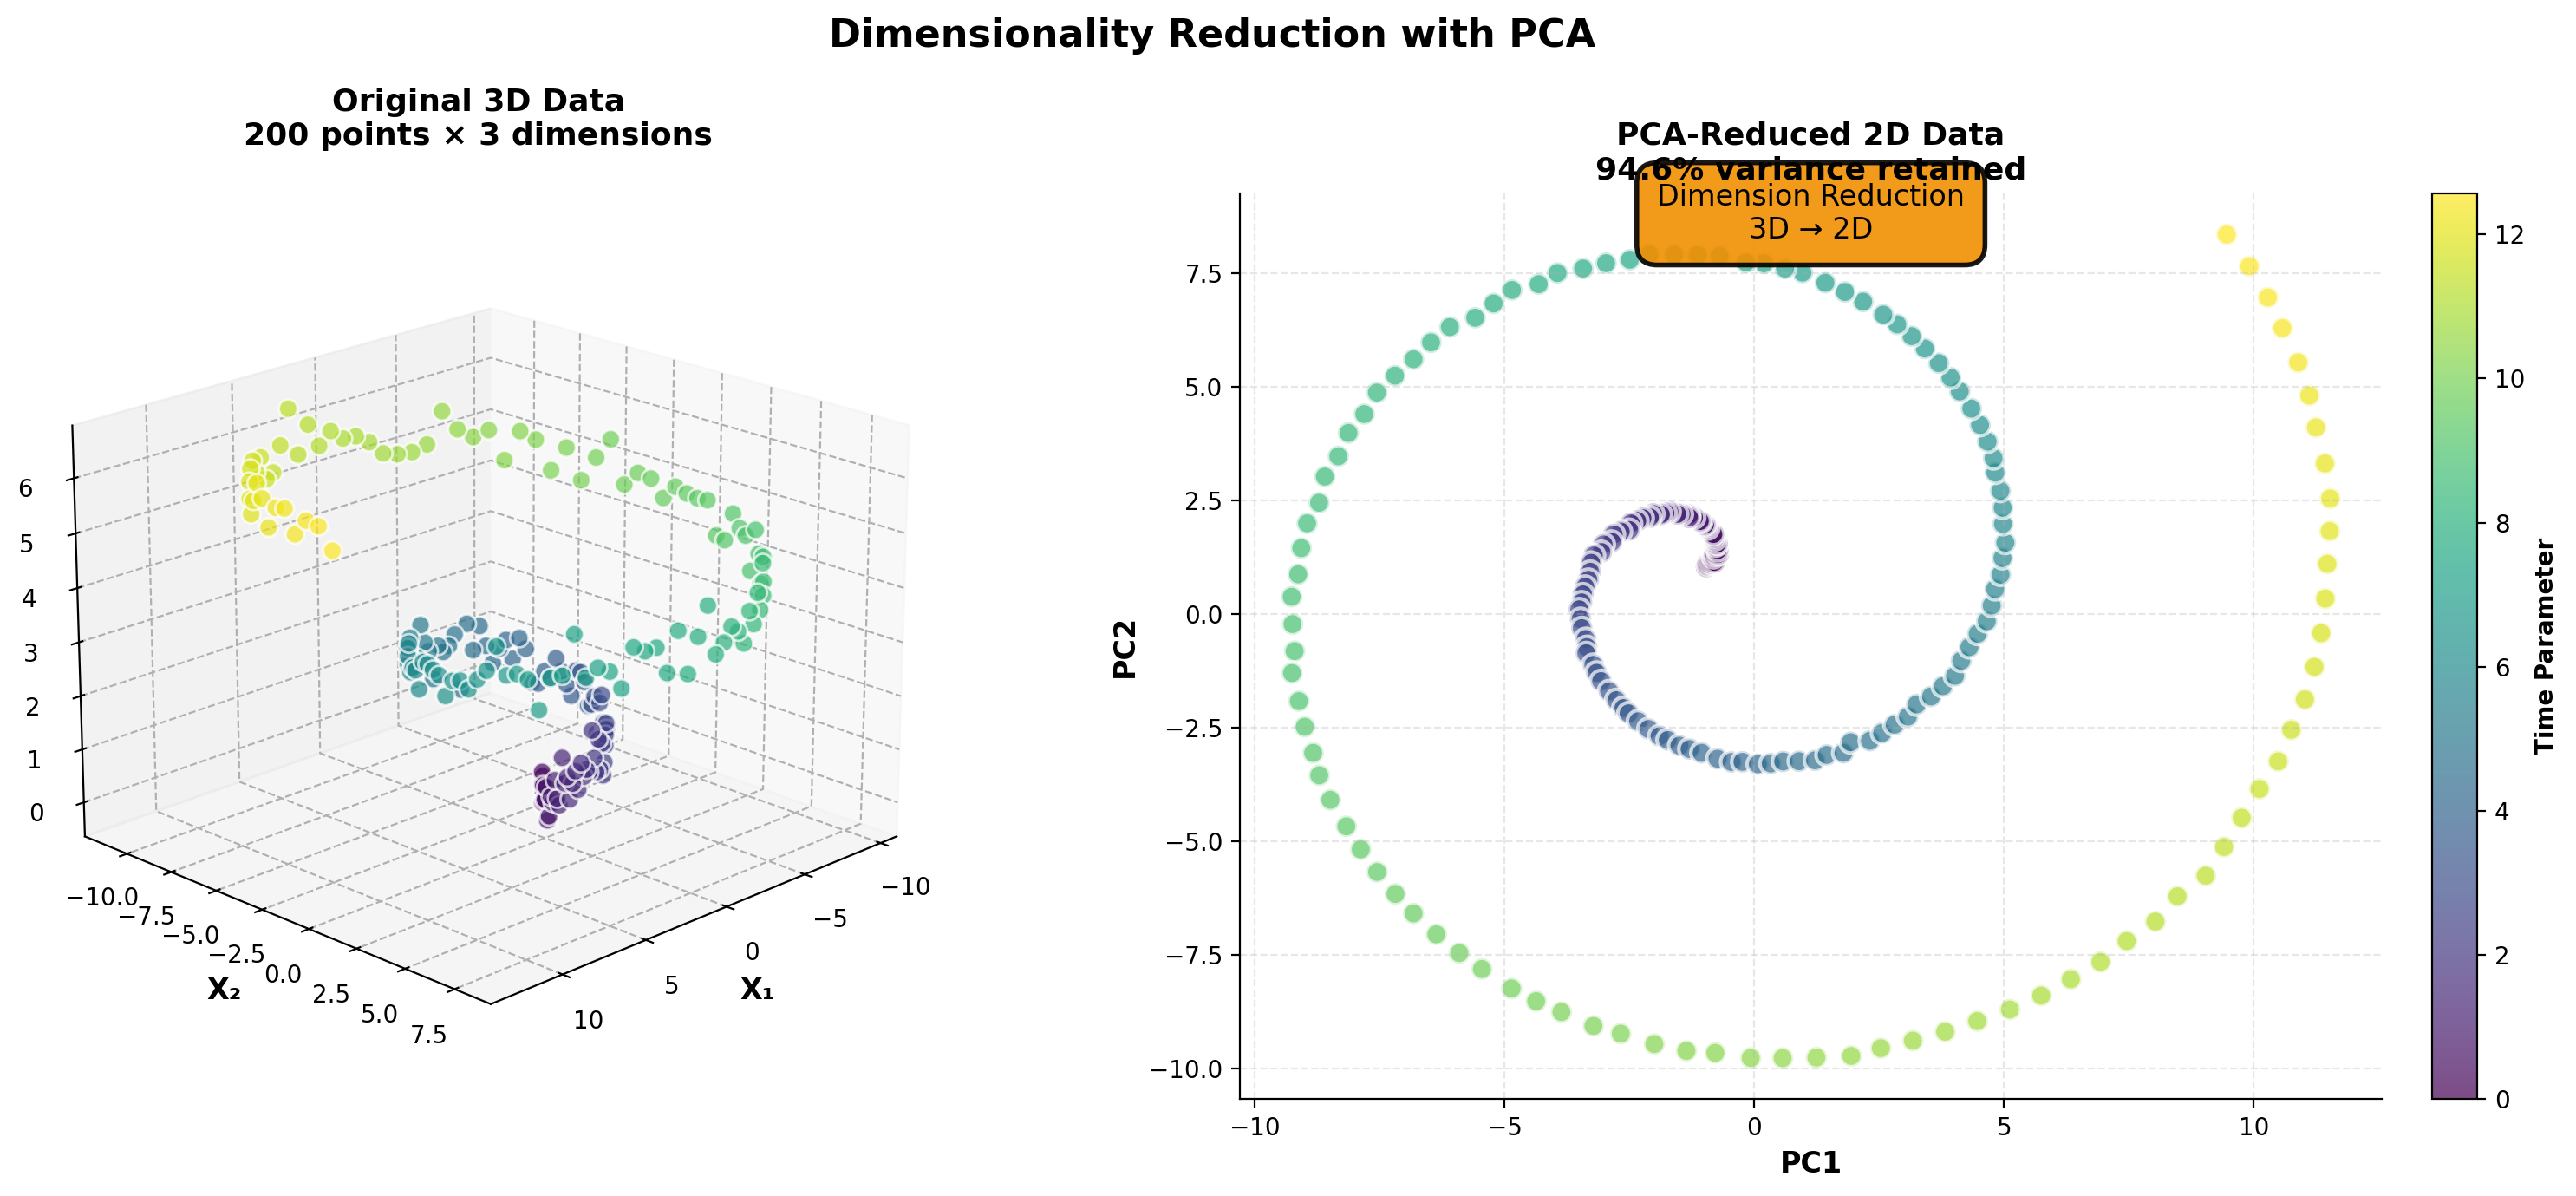
\includegraphics[width=\textwidth]{../figures/dimensionality_reduction_concept.png}

\vspace{0.2cm}

\textbf{Applications:}
\begin{itemize}
\setlength{\itemsep}{2pt}
\item Data visualization
\item Feature extraction
\item Noise reduction
\item Image compression
\end{itemize}
\end{column}
\end{columns}

\vspace{0.03cm}

\begin{alertblock}{Goal}
Find new axes (principal components) that maximize variance and are uncorrelated with each other.
\end{alertblock}
\end{frame}

\begin{frame}{The Curse of Dimensionality}
\begin{columns}[t]
\begin{column}{0.48\textwidth}
\begin{block}{Problem}
As the number of features increases, data becomes increasingly sparse, making analysis difficult and computationally expensive.
\end{block}

\vspace{0.2cm}

\textbf{Challenges in High Dimensions:}
\begin{itemize}
\setlength{\itemsep}{2pt}
\item \textbf{Data sparsity:} Points become isolated
\item \textbf{Distance measures:} Lose meaning
\item \textbf{Overfitting:} Models fit noise
\item \textbf{Computation:} Time/memory grows exponentially
\end{itemize}

\vspace{0.2cm}

\begin{alertblock}{Hughes Phenomenon}
Model performance initially improves with more features, then degrades beyond an optimal point.
\end{alertblock}
\end{column}

\begin{column}{0.48\textwidth}
\centering
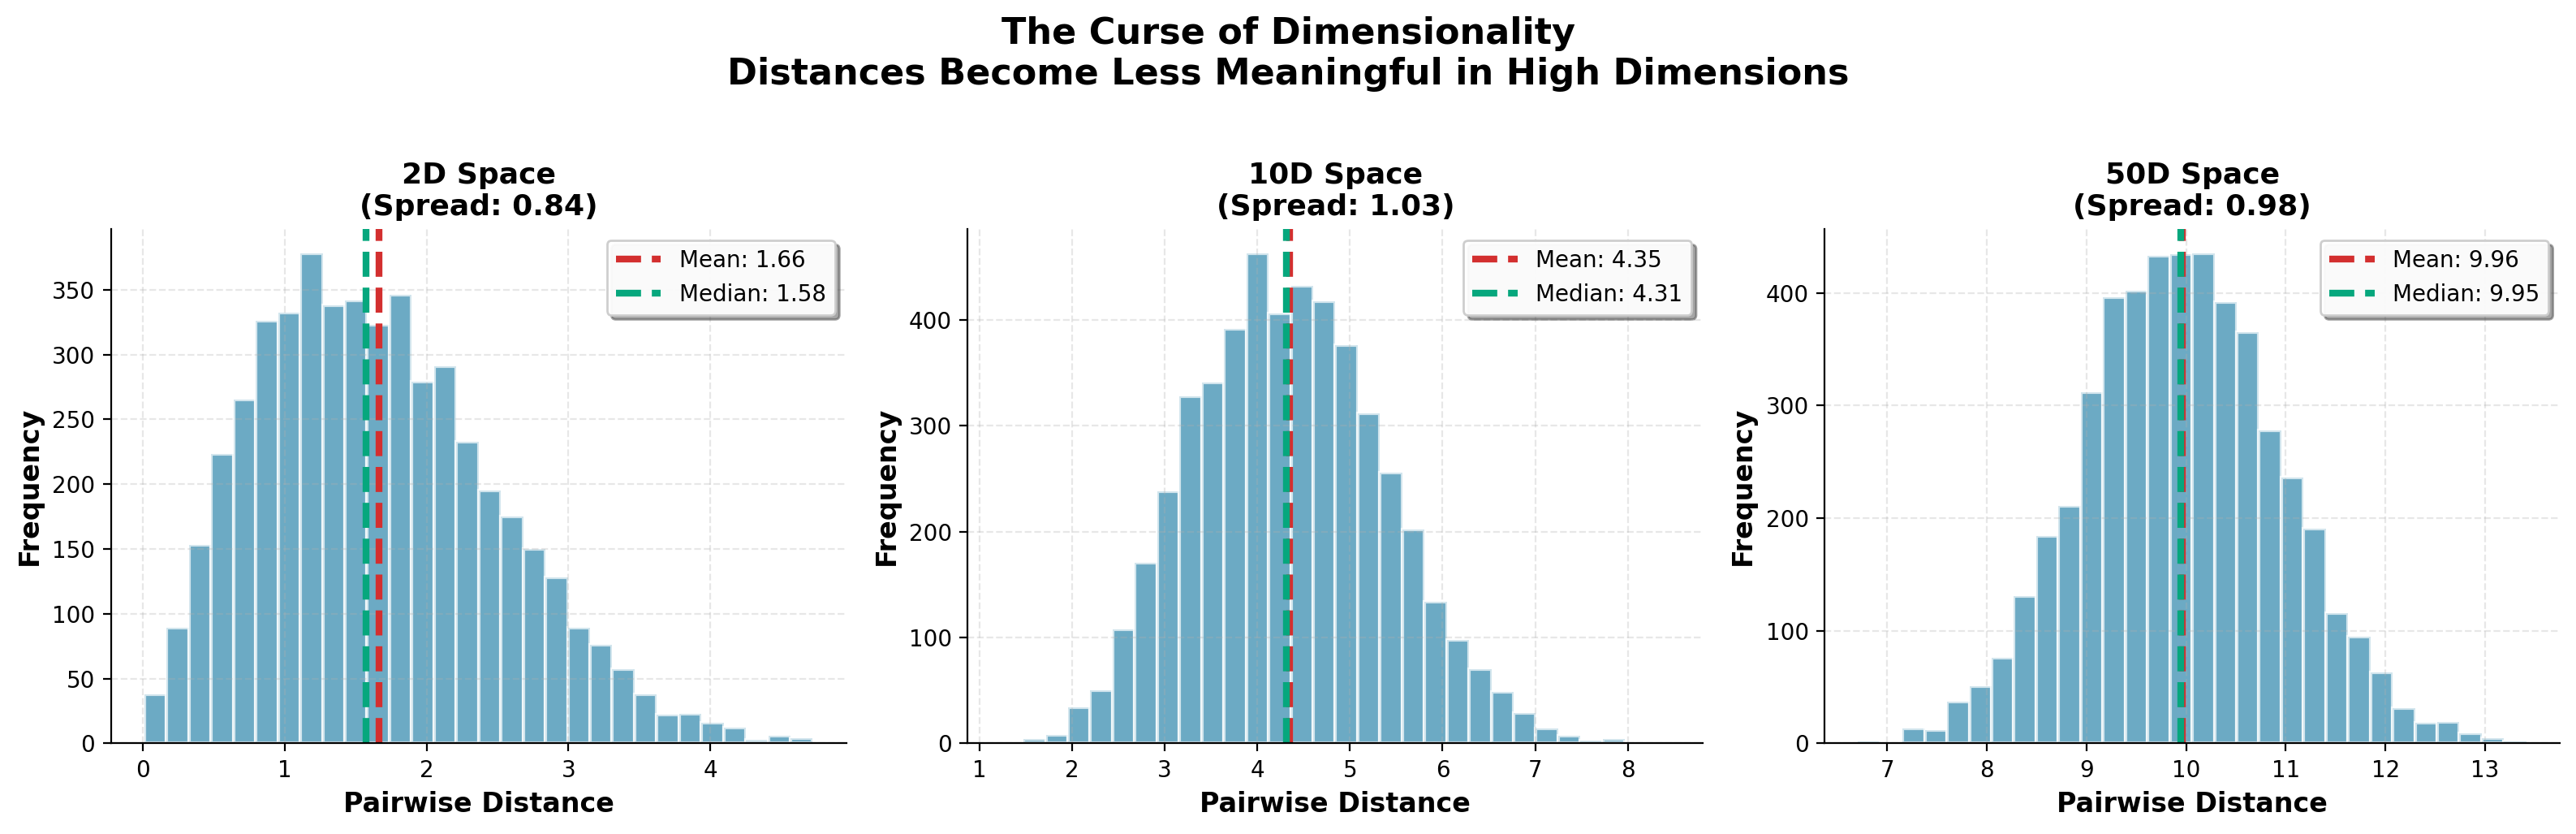
\includegraphics[width=\textwidth]{../figures/curse_of_dimensionality.png}

\vspace{0.2cm}

\textbf{Example Impact:}
\begin{itemize}
\setlength{\itemsep}{2pt}
\item 10 features: $10^2 = 100$ parameter pairs
\item 100 features: $100^2 = 10,000$ pairs
\item 1000 features: $1,000,000$ pairs!
\end{itemize}

\vspace{0.2cm}

\begin{exampleblock}{Solution: PCA}
Reduce dimensions while retaining information.
\end{exampleblock}
\end{column}
\end{columns}
\end{frame}

\begin{frame}{Why Dimensionality Reduction?}
\begin{columns}[t]
\begin{column}{0.48\textwidth}
\textbf{Motivation for PCA:}
\vspace{0.2cm}

\begin{itemize}
\setlength{\itemsep}{2pt}
\item \textbf{Visualization:} Reduce to 2D/3D for plotting
\item \textbf{Storage:} Compress data efficiently
\item \textbf{Speed:} Faster training and inference
\item \textbf{Noise removal:} Filter out low-variance components
\item \textbf{Feature extraction:} Create meaningful features
\item \textbf{Collinearity:} Remove redundant features
\end{itemize}

\vspace{0.2cm}

\begin{block}{Core Principle}
Most real-world data has intrinsic dimensionality much lower than its ambient dimensionality.
\end{block}

\vspace{0.2cm}

\textbf{Example:} Images of faces
\begin{itemize}
\setlength{\itemsep}{0pt}
\item Ambient: 10,000 pixels
\item Intrinsic: 100-200 dimensions
\end{itemize}
\end{column}

\begin{column}{0.48\textwidth}
\textbf{Benefits vs Trade-offs:}
\vspace{0.2cm}

\begin{exampleblock}{Advantages}
\begin{itemize}
\setlength{\itemsep}{2pt}
\item Reduced computational cost
\item Easier visualization
\item Noise reduction
\item Better generalization
\end{itemize}
\end{exampleblock}

\vspace{0.2cm}

\begin{alertblock}{Trade-offs}
\begin{itemize}
\setlength{\itemsep}{2pt}
\item Information loss
\item Interpretability reduced
\item Linear assumptions
\item Sensitive to scaling
\end{itemize}
\end{alertblock}

\vspace{0.2cm}

\begin{techblock}{When to Use PCA}
\begin{itemize}
\setlength{\itemsep}{0pt}
\item Many correlated features
\item Need for visualization
\item Computational constraints
\item Preprocessing for ML
\end{itemize}
\end{techblock}
\end{column}
\end{columns}
\end{frame}

\begin{frame}{Real-World Applications}
\begin{columns}[t]
\begin{column}{0.48\textwidth}
\textbf{Computer Vision:}
\begin{itemize}
\setlength{\itemsep}{2pt}
\item \textbf{Face recognition:} Eigenfaces
\item \textbf{Image compression:} Reduce storage
\item \textbf{Object detection:} Feature extraction
\item \textbf{Image denoising:} Remove noise
\end{itemize}

\vspace{0.2cm}

\textbf{Finance:}
\begin{itemize}
\setlength{\itemsep}{2pt}
\item Portfolio optimization
\item Risk assessment
\item Market trend analysis
\item Fraud detection
\end{itemize}

\vspace{0.2cm}

\textbf{Biology \& Medicine:}
\begin{itemize}
\setlength{\itemsep}{2pt}
\item Gene expression analysis
\item Medical imaging
\item Drug discovery
\item Disease classification
\end{itemize}
\end{column}

\begin{column}{0.48\textwidth}
\textbf{Natural Language Processing:}
\begin{itemize}
\setlength{\itemsep}{2pt}
\item Document clustering
\item Topic modeling
\item Sentiment analysis
\item Information retrieval
\end{itemize}

\vspace{0.2cm}

\textbf{Signal Processing:}
\begin{itemize}
\setlength{\itemsep}{2pt}
\item Audio compression
\item Speech recognition
\item Sensor data analysis
\item Anomaly detection
\end{itemize}

\vspace{0.2cm}

\textbf{Recommendation Systems:}
\begin{itemize}
\setlength{\itemsep}{2pt}
\item User preference modeling
\item Content filtering
\item Collaborative filtering
\item Feature engineering
\end{itemize}

\vspace{0.2cm}

\begin{exampleblock}{Success Story}
Netflix Prize: Teams used PCA for feature reduction and achieved significant performance gains.
\end{exampleblock}
\end{column}
\end{columns}
\end{frame}

% ========================================
% Section: Mathematical Foundations
% ========================================

\section{Mathematical Foundations}

\begin{frame}{Variance: Measuring Spread}
\begin{columns}[t]
\begin{column}{0.48\textwidth}
\begin{block}{Definition}
\textbf{Variance} measures how far data points spread from their mean value.
\end{block}

\vspace{0.2cm}

\textbf{For a single variable:}
\begin{align}
\text{Var}(X) &= \frac{1}{n}\sum_{i=1}^{n}(x_i - \bar{x})^2 \\
&= \mathbb{E}[(X - \mathbb{E}[X])^2]
\end{align}

\vspace{0.2cm}

\textbf{Properties:}
\begin{itemize}
\setlength{\itemsep}{2pt}
\item Always non-negative: $\text{Var}(X) \geq 0$
\item Zero variance: constant values
\item Units: squared original units
\item \textbf{Standard deviation:} $\sigma = \sqrt{\text{Var}(X)}$
\end{itemize}

\vspace{0.2cm}

\begin{alertblock}{PCA Goal}
Find directions of \textcolor{red}{\textbf{maximum variance}} in the data.
\end{alertblock}
\end{column}

\begin{column}{0.48\textwidth}
\centering
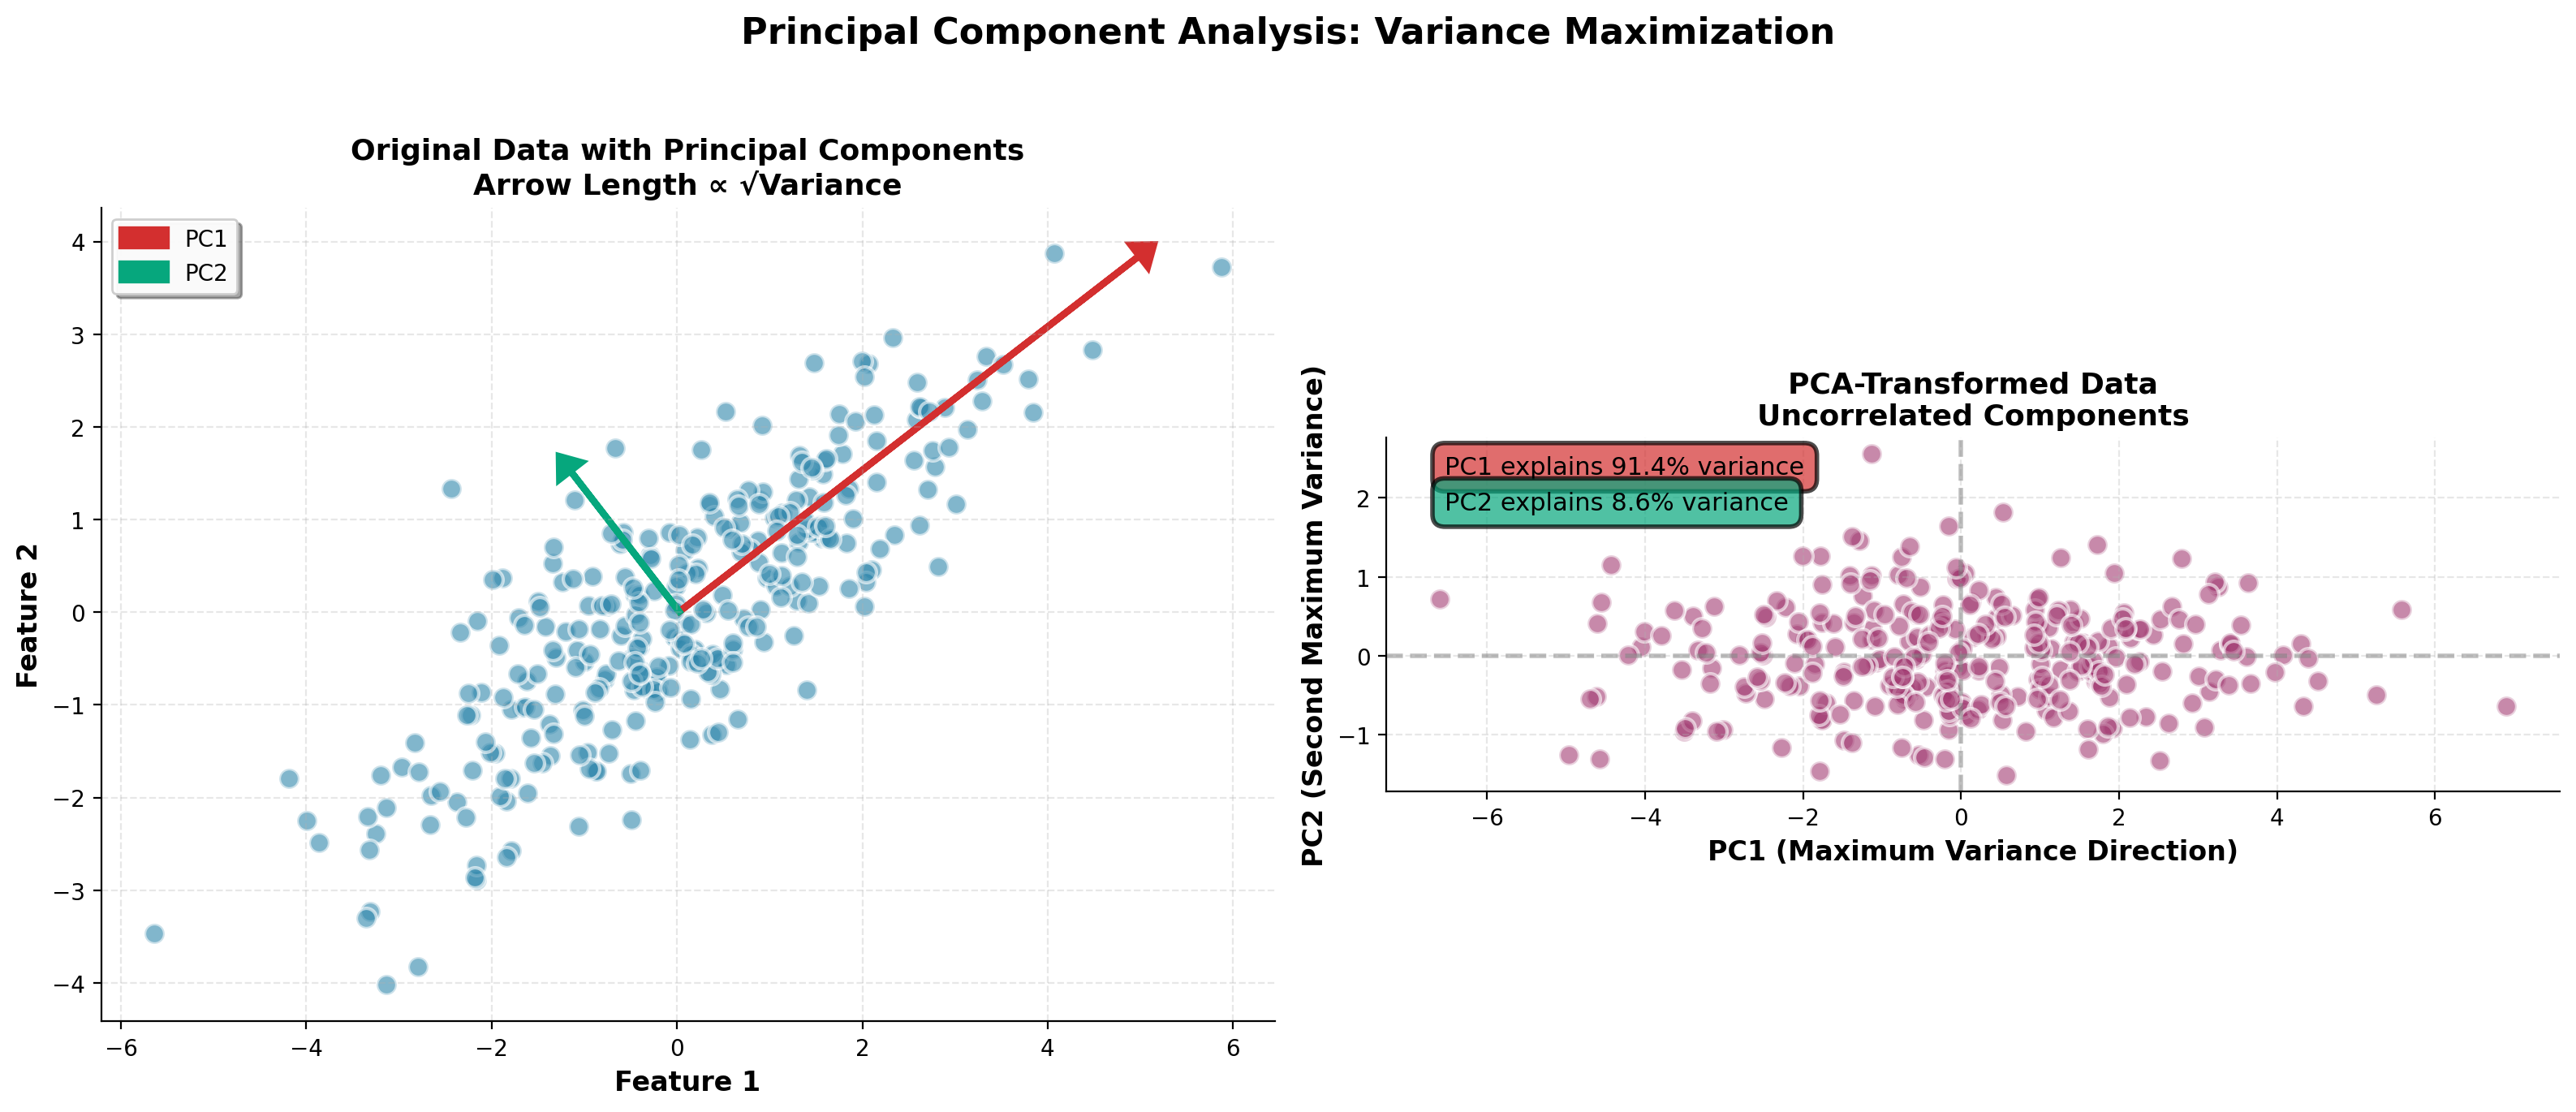
\includegraphics[width=\textwidth]{../figures/variance_visualization.png}

\vspace{0.2cm}

\textbf{Example Calculation:}

Data: $[2, 4, 6, 8, 10]$
\begin{align}
\bar{x} &= \frac{2+4+6+8+10}{5} = 6 \\
\text{Var}(X) &= \frac{(2-6)^2 + (4-6)^2 + \cdots}{5} \\
&= \frac{16 + 4 + 0 + 4 + 16}{5} = 8
\end{align}

\vspace{0.2cm}

\begin{exampleblock}{Intuition}
High variance direction contains more information than low variance direction.
\end{exampleblock}
\end{column}
\end{columns}
\end{frame}

\begin{frame}{Covariance: Measuring Linear Relationship}
\begin{columns}[t]
\begin{column}{0.48\textwidth}
\begin{block}{Definition}
\textbf{Covariance} measures the joint variability of two variables.
\end{block}

\vspace{0.2cm}

\textbf{Formula:}
\begin{align}
\text{Cov}(X, Y) &= \frac{1}{n}\sum_{i=1}^{n}(x_i - \bar{x})(y_i - \bar{y}) \\
&= \mathbb{E}[(X - \mathbb{E}[X])(Y - \mathbb{E}[Y])]
\end{align}

\vspace{0.2cm}

\textbf{Interpretation:}
\begin{itemize}
\setlength{\itemsep}{2pt}
\item $\text{Cov}(X, Y) > 0$: Positive relationship
\item $\text{Cov}(X, Y) < 0$: Negative relationship
\item $\text{Cov}(X, Y) = 0$: No linear relationship
\item $\text{Cov}(X, X) = \text{Var}(X)$
\end{itemize}

\vspace{0.2cm}

\begin{exampleblock}{Correlation}
Normalized covariance:
$$\rho_{XY} = \frac{\text{Cov}(X,Y)}{\sigma_X \sigma_Y} \in [-1, 1]$$
\end{exampleblock}
\end{column}

\begin{column}{0.48\textwidth}
\textbf{Covariance Matrix:}

For data $\mathbf{X} \in \mathbb{R}^{n \times d}$:
$$\mathbf{\Sigma} = \frac{1}{n}\mathbf{X}^T\mathbf{X} \in \mathbb{R}^{d \times d}$$

\vspace{0.2cm}

\textbf{Structure:}
$$\mathbf{\Sigma} = \begin{bmatrix}
\text{Var}(X_1) & \text{Cov}(X_1,X_2) & \cdots \\
\text{Cov}(X_2,X_1) & \text{Var}(X_2) & \cdots \\
\vdots & \vdots & \ddots
\end{bmatrix}$$

\vspace{0.2cm}

\textbf{Properties:}
\begin{itemize}
\setlength{\itemsep}{2pt}
\item Symmetric: $\Sigma_{ij} = \Sigma_{ji}$
\item Positive semi-definite
\item Diagonal: variances
\item Off-diagonal: covariances
\end{itemize}

\vspace{0.2cm}

\begin{alertblock}{PCA Key}
Diagonalize covariance matrix to find uncorrelated components.
\end{alertblock}
\end{column}
\end{columns}
\end{frame}

\begin{frame}{Eigendecomposition: The Core of PCA}
\begin{columns}[t]
\begin{column}{0.48\textwidth}
\begin{block}{Definition}
For a square matrix $\mathbf{A}$, \textbf{eigendecomposition} finds vectors and scalars such that:
$$\mathbf{A}\mathbf{v} = \lambda \mathbf{v}$$
\end{block}

\vspace{0.2cm}

\textbf{Components:}
\begin{itemize}
\setlength{\itemsep}{2pt}
\item $\mathbf{v}$: \textcolor{blue}{\textbf{Eigenvector}} (direction)
\item $\lambda$: \textcolor{red}{\textbf{Eigenvalue}} (scaling factor)
\item Matrix only changes \textit{magnitude}, not direction
\end{itemize}

\vspace{0.2cm}

\textbf{For Covariance Matrix:}
$$\mathbf{\Sigma} = \mathbf{V}\mathbf{\Lambda}\mathbf{V}^T$$

where:
\begin{itemize}
\setlength{\itemsep}{0pt}
\item $\mathbf{V}$: Eigenvector matrix
\item $\mathbf{\Lambda}$: Diagonal eigenvalue matrix
\item $\mathbf{V}^T\mathbf{V} = \mathbf{I}$ (orthonormal)
\end{itemize}
\end{column}

\begin{column}{0.48\textwidth}
\centering
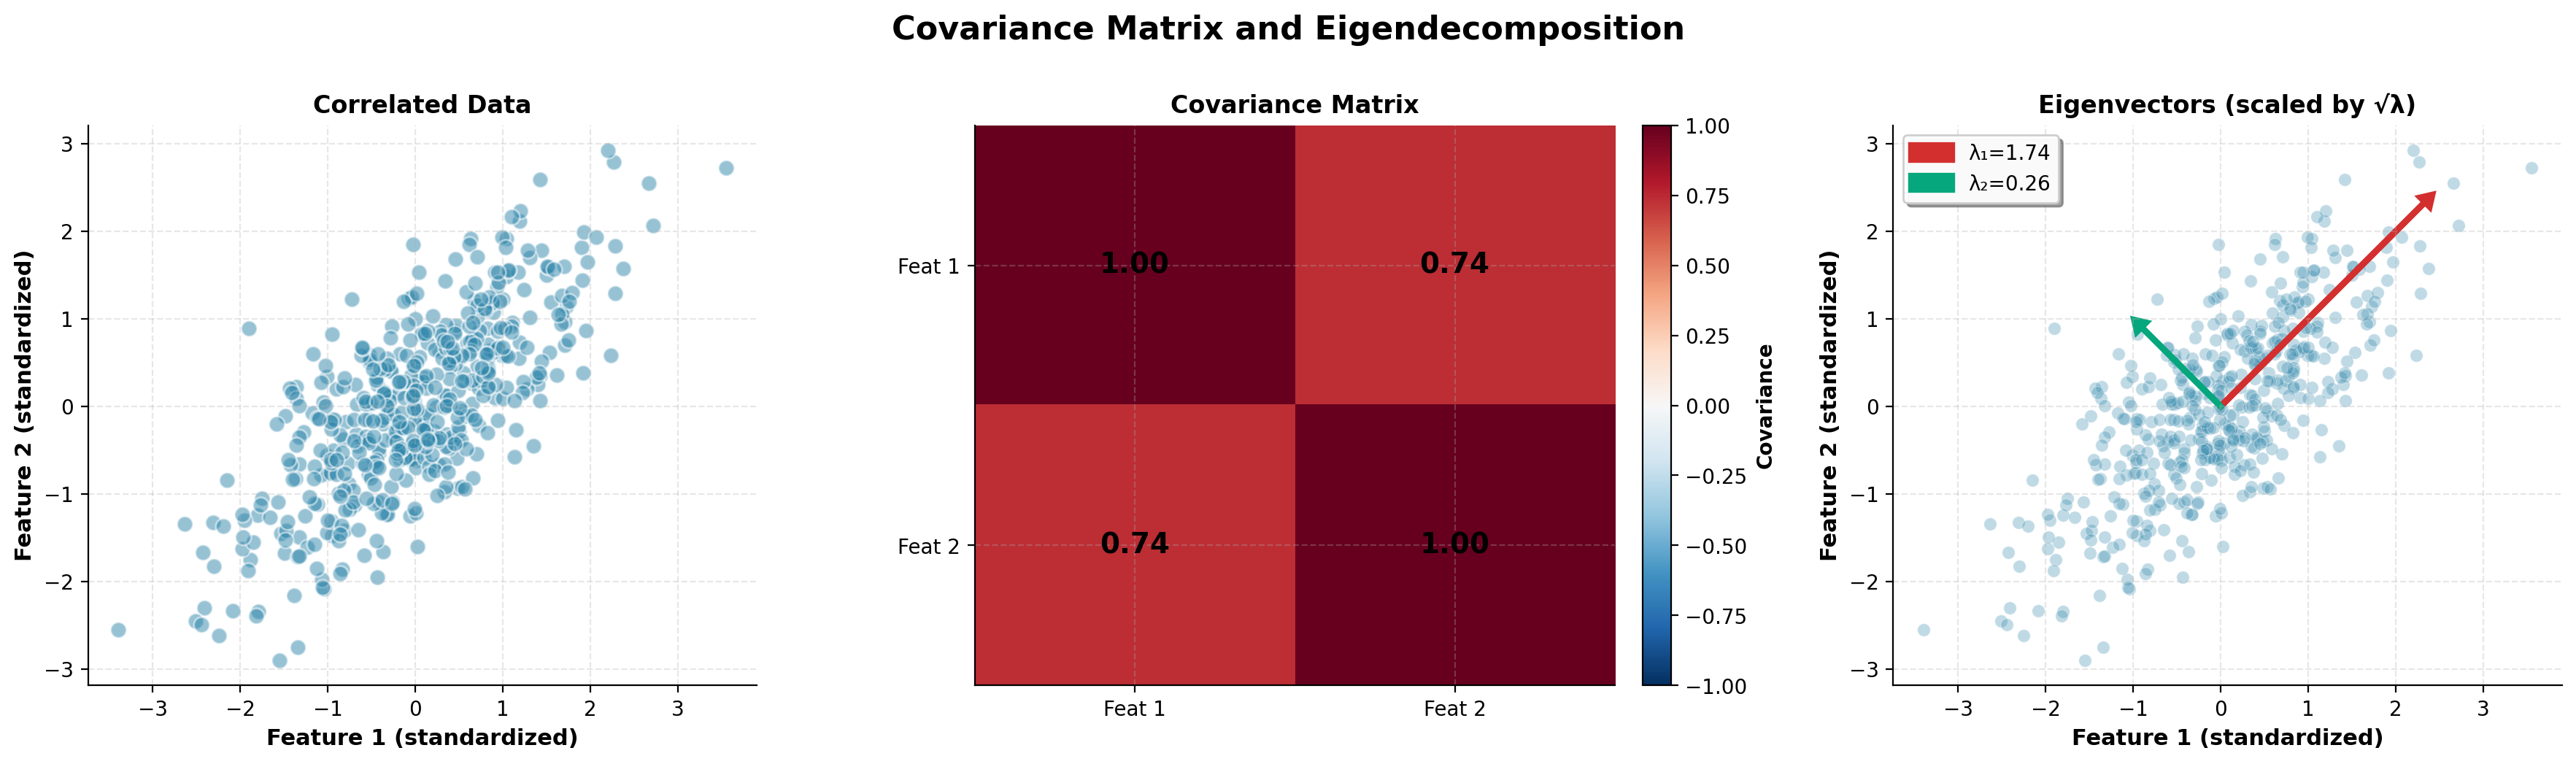
\includegraphics[width=\textwidth]{../figures/covariance_eigenvectors.png}

\vspace{0.2cm}

\textbf{Geometric Interpretation:}
\begin{itemize}
\setlength{\itemsep}{2pt}
\item Eigenvectors: Principal component directions
\item Eigenvalues: Variance along each PC
\item Largest eigenvalue: Most variance
\item Smallest eigenvalue: Least variance
\end{itemize}

\vspace{0.2cm}

\begin{exampleblock}{PCA Connection}
\begin{itemize}
\setlength{\itemsep}{0pt}
\item PC directions = Eigenvectors
\item PC importance = Eigenvalues
\item Sorted by decreasing eigenvalue
\end{itemize}
\end{exampleblock}
\end{column}
\end{columns}
\end{frame}

\begin{frame}{Eigendecomposition Example}
\begin{columns}[t]
\begin{column}{0.48\textwidth}
\textbf{Problem:} Find eigenvalues and eigenvectors

$$\mathbf{\Sigma} = \begin{bmatrix} 4 & 2 \\ 2 & 3 \end{bmatrix}$$

\vspace{0.2cm}

\textbf{Step 1: Characteristic equation}
$$\det(\mathbf{\Sigma} - \lambda \mathbf{I}) = 0$$

$$\det\begin{bmatrix} 4-\lambda & 2 \\ 2 & 3-\lambda \end{bmatrix} = 0$$

$$(4-\lambda)(3-\lambda) - 4 = 0$$
$$\lambda^2 - 7\lambda + 8 = 0$$

\vspace{0.2cm}

\textbf{Step 2: Solve for eigenvalues}
$$\lambda_1 = 5.56, \quad \lambda_2 = 1.44$$
\end{column}

\begin{column}{0.48\textwidth}
\textbf{Step 3: Find eigenvectors}

For $\lambda_1 = 5.56$:
$$(\mathbf{\Sigma} - 5.56\mathbf{I})\mathbf{v}_1 = 0$$
$$\mathbf{v}_1 = \begin{bmatrix} 0.79 \\ 0.61 \end{bmatrix}$$

For $\lambda_2 = 1.44$:
$$\mathbf{v}_2 = \begin{bmatrix} -0.61 \\ 0.79 \end{bmatrix}$$

\vspace{0.2cm}

\textbf{Interpretation:}
\begin{itemize}
\setlength{\itemsep}{2pt}
\item PC1 direction: $(0.79, 0.61)$
\item PC1 variance: $5.56$
\item PC2 direction: $(-0.61, 0.79)$
\item PC2 variance: $1.44$
\item Total variance: $5.56 + 1.44 = 7$
\end{itemize}

\vspace{0.2cm}

\begin{alertblock}{Note}
Eigenvectors are orthogonal: $\mathbf{v}_1 \perp \mathbf{v}_2$
\end{alertblock}
\end{column}
\end{columns}
\end{frame}

\begin{frame}{Singular Value Decomposition (SVD)}
\begin{columns}[t]
\begin{column}{0.48\textwidth}
\begin{block}{Definition}
Any matrix $\mathbf{X} \in \mathbb{R}^{n \times d}$ can be decomposed as:
$$\mathbf{X} = \mathbf{U}\mathbf{\Sigma}\mathbf{V}^T$$
\end{block}

\vspace{0.2cm}

\textbf{Components:}
\begin{itemize}
\setlength{\itemsep}{2pt}
\item $\mathbf{U} \in \mathbb{R}^{n \times n}$: Left singular vectors
\item $\mathbf{\Sigma} \in \mathbb{R}^{n \times d}$: Singular values (diagonal)
\item $\mathbf{V} \in \mathbb{R}^{d \times d}$: Right singular vectors
\item $\mathbf{U}^T\mathbf{U} = \mathbf{I}$, $\mathbf{V}^T\mathbf{V} = \mathbf{I}$
\end{itemize}

\vspace{0.2cm}

\textbf{Relationship to PCA:}
$$\mathbf{X}^T\mathbf{X} = \mathbf{V}\mathbf{\Sigma}^T\mathbf{\Sigma}\mathbf{V}^T$$

Therefore:
\begin{itemize}
\setlength{\itemsep}{0pt}
\item PC directions: Columns of $\mathbf{V}$
\item PC variances: $\sigma_i^2 / n$
\end{itemize}
\end{column}

\begin{column}{0.48\textwidth}
\centering
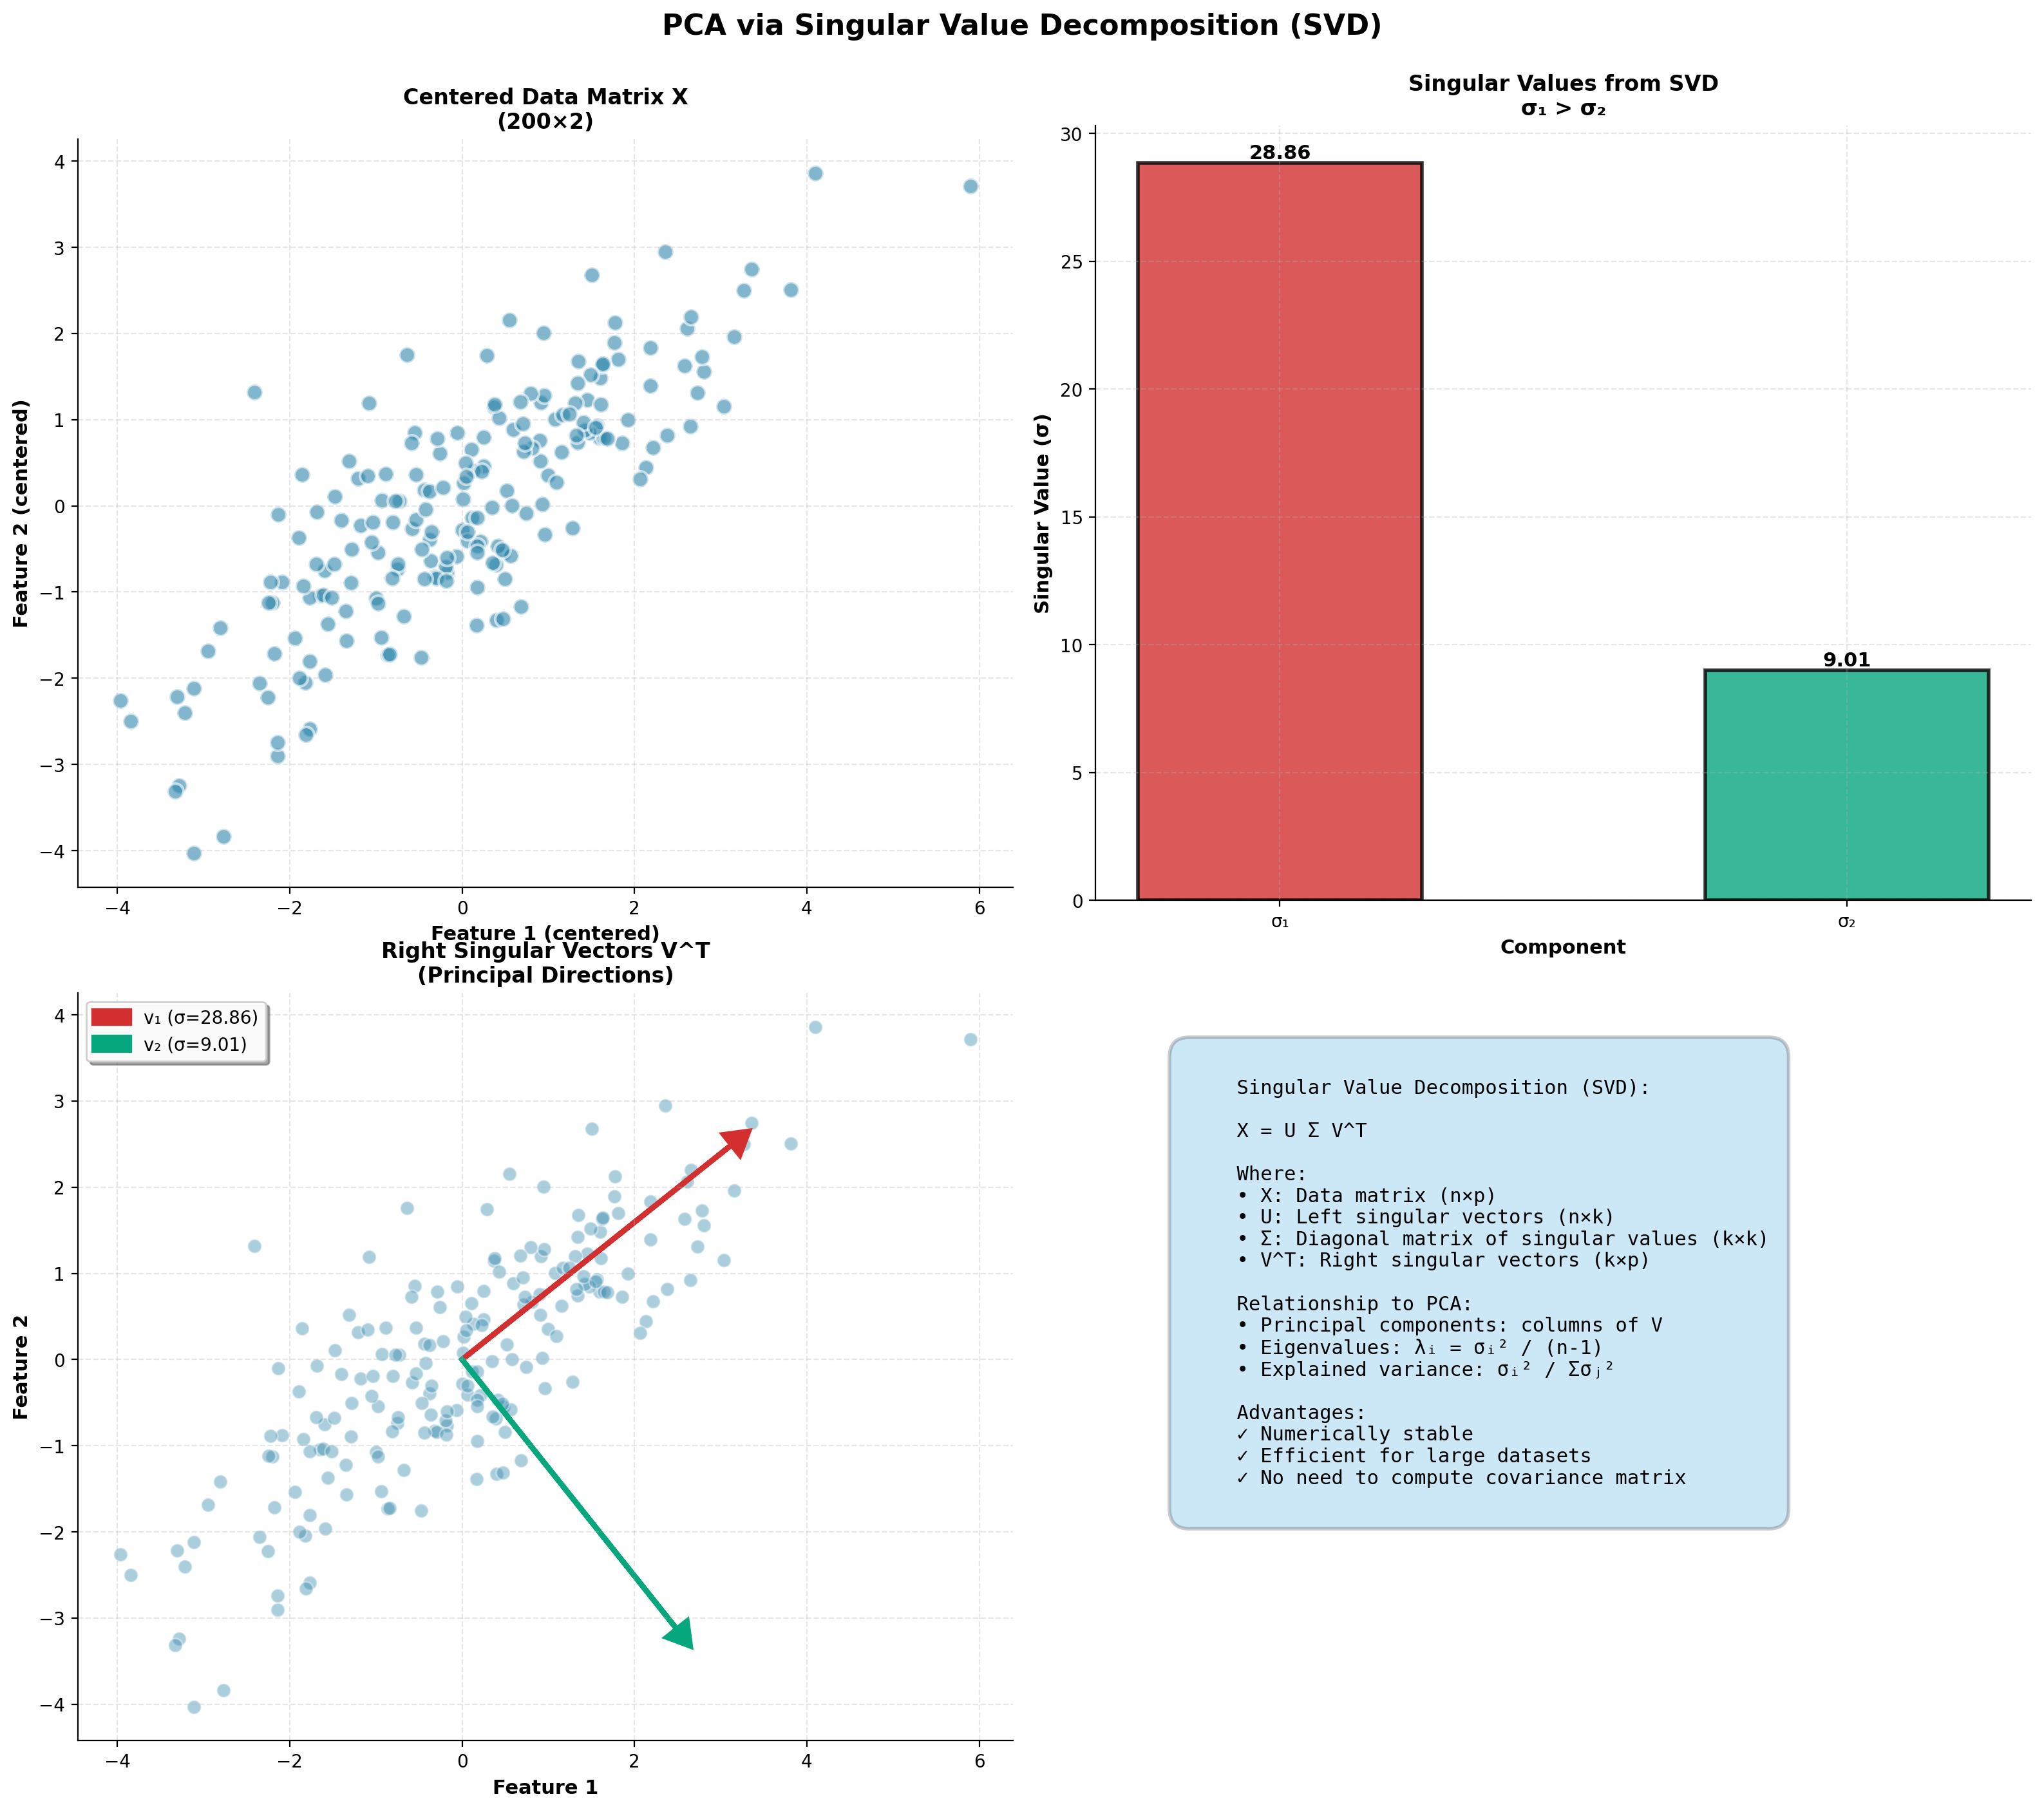
\includegraphics[width=\textwidth]{../figures/svd_decomposition.png}

\vspace{0.2cm}

\textbf{Advantages of SVD for PCA:}
\begin{itemize}
\setlength{\itemsep}{2pt}
\item More numerically stable
\item Works for $n < d$ or $n > d$
\item No need to form $\mathbf{X}^T\mathbf{X}$
\item Efficient algorithms available
\end{itemize}

\vspace{0.2cm}

\begin{exampleblock}{Truncated SVD}
Keep only top $k$ components:
$$\mathbf{X}_k = \mathbf{U}_k\mathbf{\Sigma}_k\mathbf{V}_k^T$$
Best rank-$k$ approximation in Frobenius norm.
\end{exampleblock}
\end{column}
\end{columns}
\end{frame}

\begin{frame}{SVD vs Eigendecomposition}
\begin{columns}[t]
\begin{column}{0.48\textwidth}
\begin{block}{Eigendecomposition Approach}
\textbf{Steps:}
\begin{enumerate}
\setlength{\itemsep}{2pt}
\item Center data: $\tilde{\mathbf{X}} = \mathbf{X} - \bar{\mathbf{X}}$
\item Compute covariance: $\mathbf{\Sigma} = \frac{1}{n}\tilde{\mathbf{X}}^T\tilde{\mathbf{X}}$
\item Eigendecomposition: $\mathbf{\Sigma} = \mathbf{V}\mathbf{\Lambda}\mathbf{V}^T$
\item Sort by eigenvalues
\end{enumerate}

\vspace{0.2cm}

\textbf{Complexity:} $\mathcal{O}(d^2n + d^3)$

\vspace{0.2cm}

\textbf{Issues:}
\begin{itemize}
\setlength{\itemsep}{2pt}
\item Numerical instability for $\mathbf{X}^T\mathbf{X}$
\item Squaring condition number
\item Memory: storing $d \times d$ matrix
\end{itemize}
\end{block}
\end{column}

\begin{column}{0.48\textwidth}
\begin{block}{SVD Approach}
\textbf{Steps:}
\begin{enumerate}
\setlength{\itemsep}{2pt}
\item Center data: $\tilde{\mathbf{X}} = \mathbf{X} - \bar{\mathbf{X}}$
\item SVD: $\tilde{\mathbf{X}} = \mathbf{U}\mathbf{\Sigma}\mathbf{V}^T$
\item PCs: columns of $\mathbf{V}$
\item Variance: $\sigma_i^2 / n$
\end{enumerate}

\vspace{0.2cm}

\textbf{Complexity:} $\mathcal{O}(\min(nd^2, n^2d))$

\vspace{0.2cm}

\textbf{Advantages:}
\begin{itemize}
\setlength{\itemsep}{2pt}
\item Better numerical stability
\item Works directly on $\mathbf{X}$
\item Better for $n \ll d$ or $n \gg d$
\item Modern implementations optimized
\end{itemize}
\end{block}

\vspace{0.2cm}

\begin{alertblock}{Recommendation}
Use SVD for PCA in practice.
\end{alertblock}
\end{column}
\end{columns}
\end{frame}

\begin{frame}{Projection and Reconstruction}
\begin{columns}[t]
\begin{column}{0.48\textwidth}
\textbf{Projection onto PCs:}

Transform to $k$ principal components:
$$\mathbf{Z} = \mathbf{X}\mathbf{V}_k$$

where $\mathbf{V}_k \in \mathbb{R}^{d \times k}$ are first $k$ PCs.

\vspace{0.2cm}

\textbf{Properties:}
\begin{itemize}
\setlength{\itemsep}{2pt}
\item $\mathbf{Z} \in \mathbb{R}^{n \times k}$: Reduced representation
\item Columns of $\mathbf{Z}$ are uncorrelated
\item Maximum variance preserved
\item Linear transformation
\end{itemize}

\vspace{0.2cm}

\textbf{Reconstruction:}
$$\hat{\mathbf{X}} = \mathbf{Z}\mathbf{V}_k^T = \mathbf{X}\mathbf{V}_k\mathbf{V}_k^T$$

\vspace{0.2cm}

\begin{alertblock}{Reconstruction Error}
$$\|\mathbf{X} - \hat{\mathbf{X}}\|_F^2 = \sum_{i=k+1}^{d}\lambda_i$$
\end{alertblock}
\end{column}

\begin{column}{0.48\textwidth}
\centering
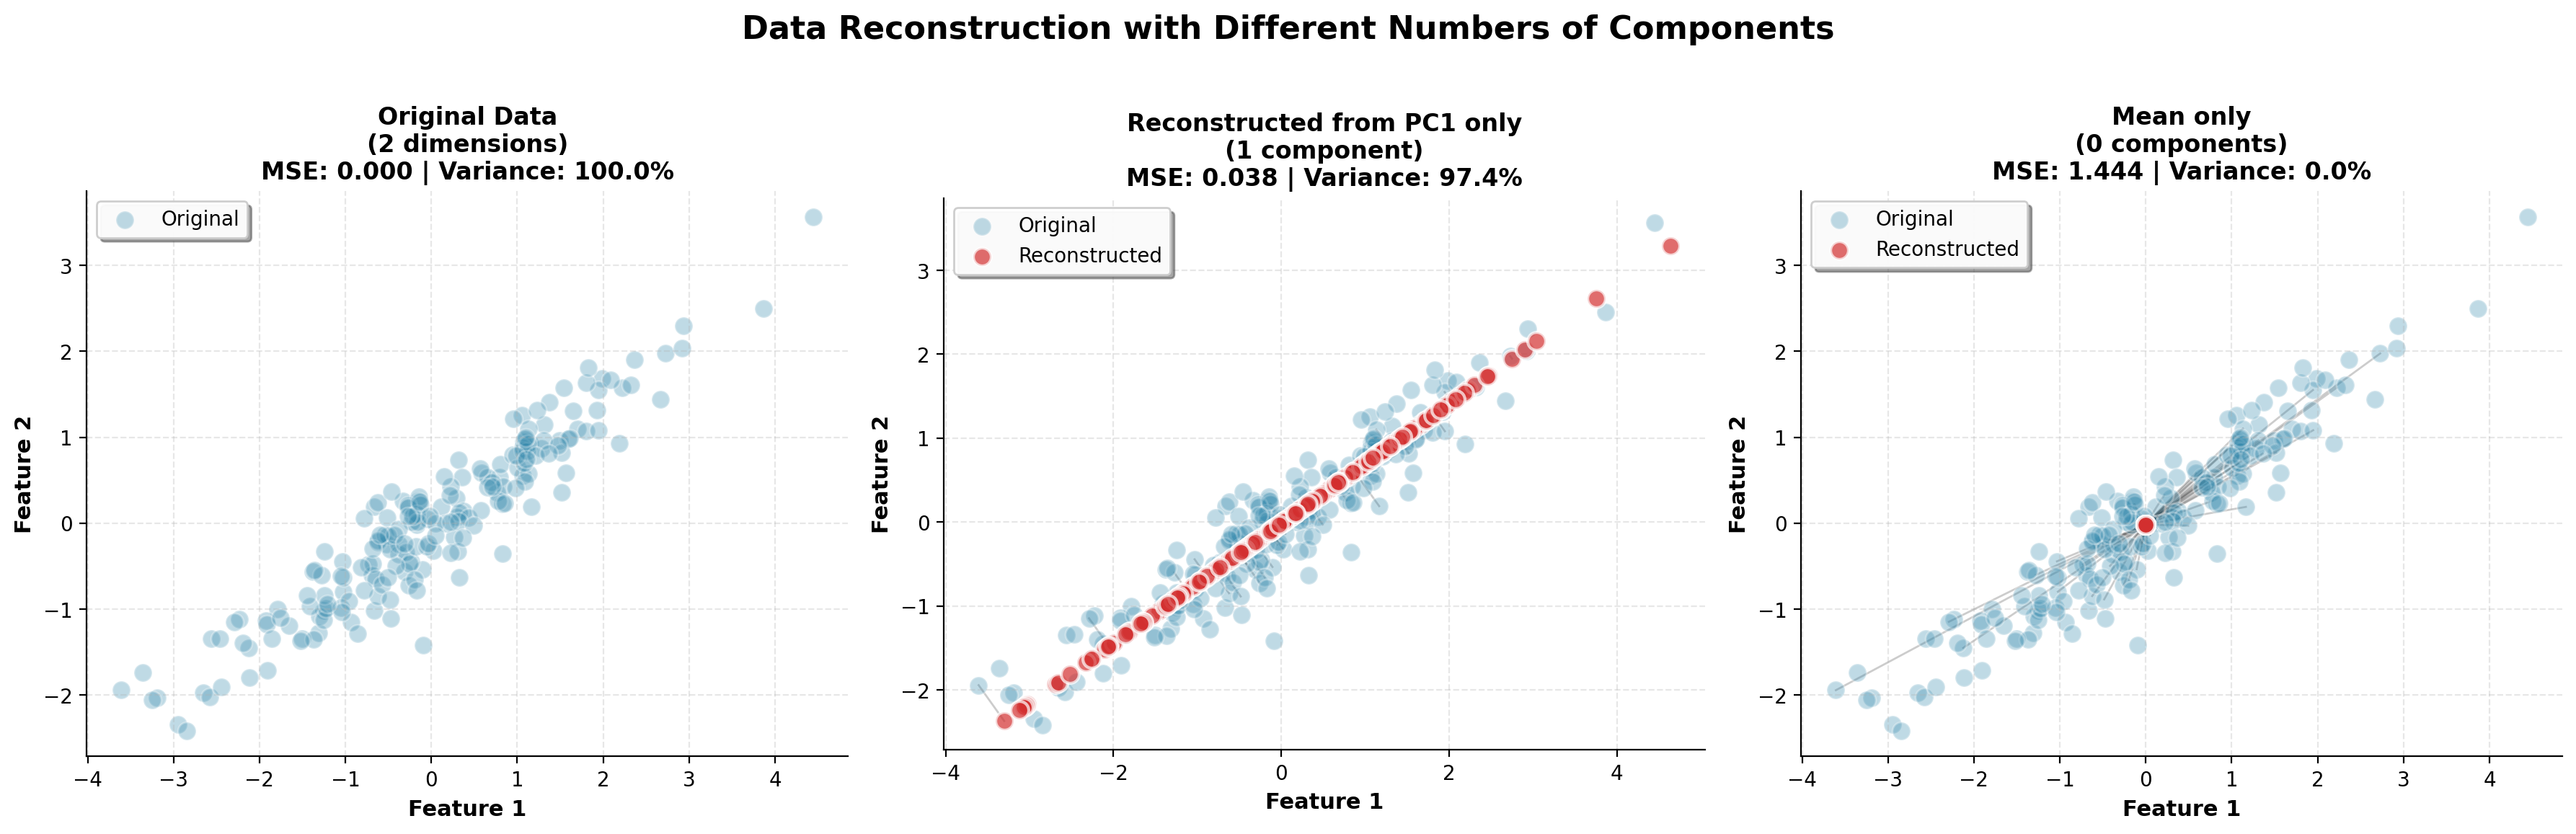
\includegraphics[width=\textwidth]{../figures/pca_reconstruction.png}

\vspace{0.2cm}

\textbf{Example:}

Original: $\mathbf{x} = [5, 3]$

PCs: $\mathbf{v}_1 = [0.8, 0.6]$

Projection:
$$z_1 = \mathbf{x}^T\mathbf{v}_1 = 5(0.8) + 3(0.6) = 5.8$$

Reconstruction:
$$\hat{\mathbf{x}} = z_1\mathbf{v}_1 = 5.8[0.8, 0.6] = [4.64, 3.48]$$

Error:
$$\|\mathbf{x} - \hat{\mathbf{x}}\| = \|[0.36, -0.48]\| = 0.6$$
\end{column}
\end{columns}
\end{frame}

\begin{frame}{Data Centering and Standardization}
\begin{columns}[t]
\begin{column}{0.48\textwidth}
\textbf{Centering (Required):}

Remove mean from each feature:
$$\tilde{x}_{ij} = x_{ij} - \bar{x}_j$$

\vspace{0.2cm}

\textbf{Why?}
\begin{itemize}
\setlength{\itemsep}{2pt}
\item PCA finds directions of variance
\item Variance computed about mean
\item Ensures PC1 passes through origin
\item Mathematical requirement
\end{itemize}

\vspace{0.2cm}

\textbf{Standardization (Optional):}

Scale to unit variance:
$$\tilde{x}_{ij} = \frac{x_{ij} - \bar{x}_j}{\sigma_j}$$

\vspace{0.2cm}

\textbf{When to standardize?}
\begin{itemize}
\setlength{\itemsep}{2pt}
\item Features have different scales
\item Different units of measurement
\item Want equal feature importance
\end{itemize}
\end{column}

\begin{column}{0.48\textwidth}
\centering
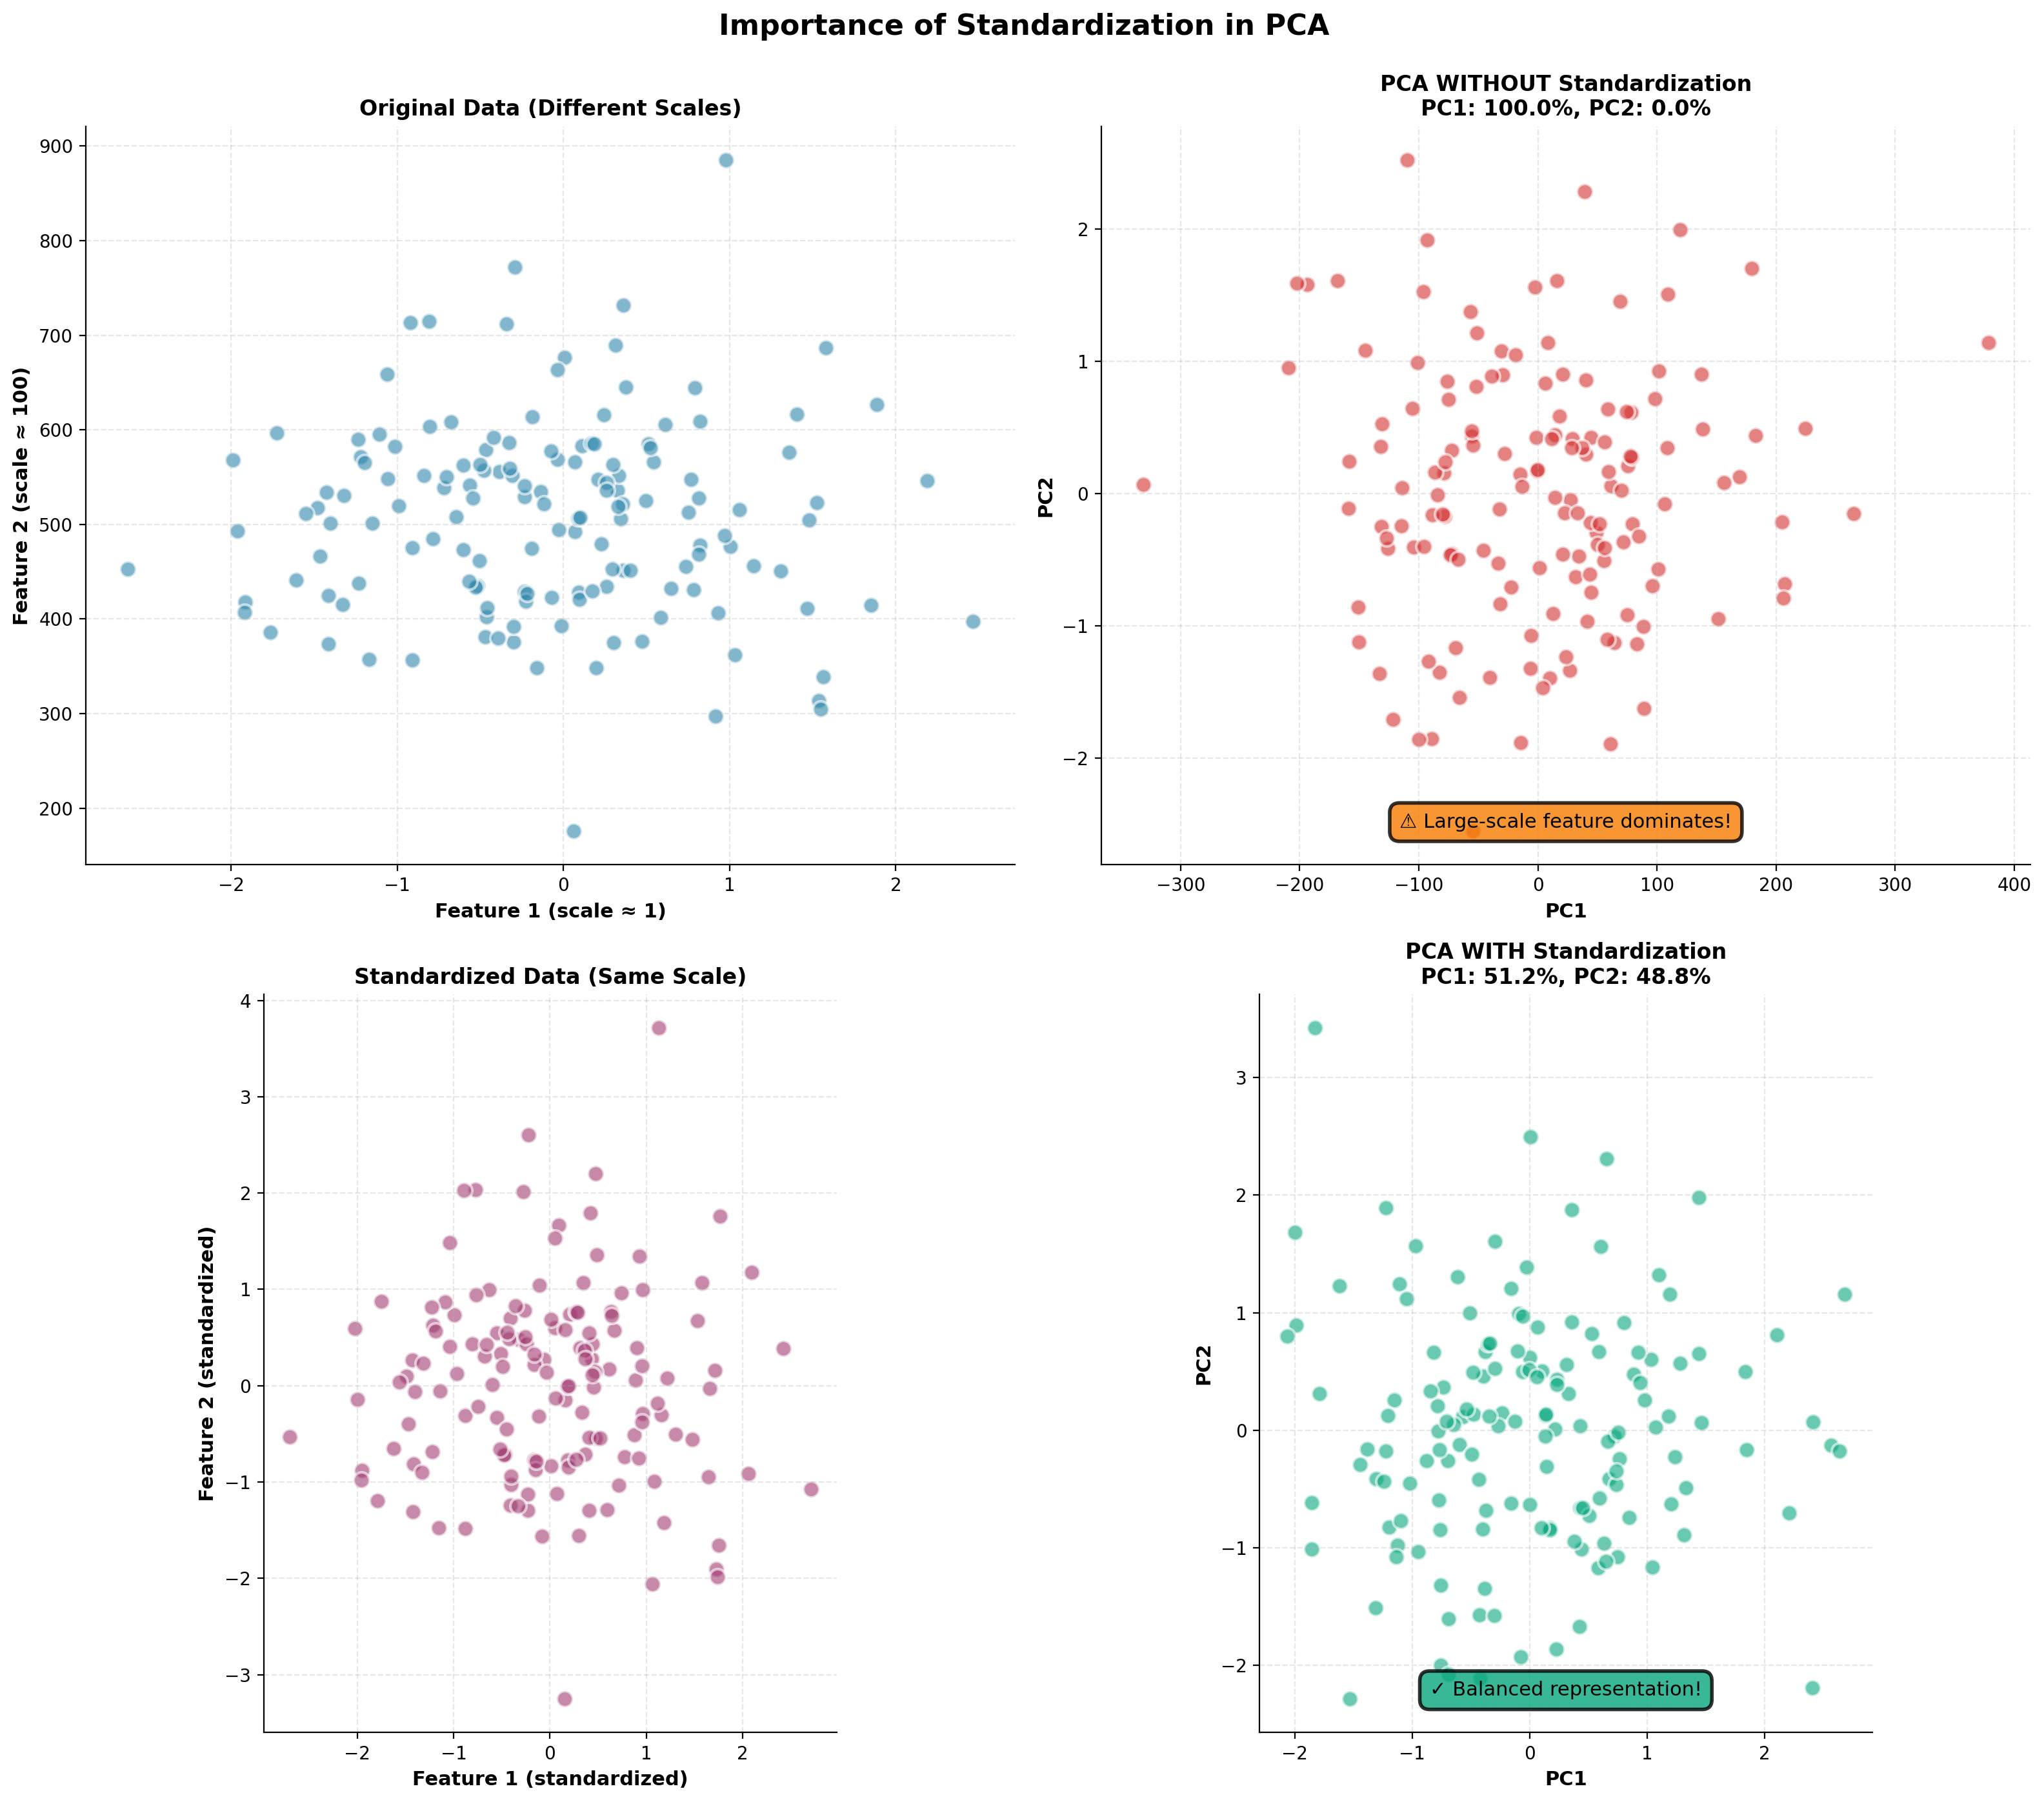
\includegraphics[width=\textwidth]{../figures/standardization_importance.png}

\vspace{0.2cm}

\begin{exampleblock}{Example Impact}
Without standardization:
\begin{itemize}
\setlength{\itemsep}{0pt}
\item Income: \$20,000-\$200,000
\item Age: 20-80 years
\item PC1 dominated by income scale
\end{itemize}

With standardization:
\begin{itemize}
\setlength{\itemsep}{0pt}
\item Both scaled to mean 0, std 1
\item Equal contribution opportunity
\end{itemize}
\end{exampleblock}

\vspace{0.2cm}

\begin{alertblock}{Best Practice}
\textbf{Always center.} Standardize if features have different scales or units.
\end{alertblock}
\end{column}
\end{columns}
\end{frame}

% ========================================
% Section: PCA Algorithm
% ========================================

\section{The PCA Algorithm}

\begin{frame}{PCA Algorithm: Step-by-Step}
\begin{columns}[t]
\begin{column}{0.48\textwidth}
\begin{algorithm}[H]
\caption{Principal Component Analysis}
\begin{algorithmic}[1]
\REQUIRE Data matrix $\mathbf{X} \in \mathbb{R}^{n \times d}$, number of components $k$
\ENSURE Principal components $\mathbf{V}_k$, transformed data $\mathbf{Z}$
\STATE \textbf{Center} the data:
\STATE $\bar{\mathbf{x}} = \frac{1}{n}\sum_{i=1}^{n}\mathbf{x}_i$
\STATE $\tilde{\mathbf{X}} = \mathbf{X} - \mathbf{1}_n\bar{\mathbf{x}}^T$
\STATE \textbf{Optional:} Standardize features
\STATE \textbf{Compute} covariance matrix:
\STATE $\mathbf{\Sigma} = \frac{1}{n}\tilde{\mathbf{X}}^T\tilde{\mathbf{X}}$
\STATE \textbf{OR} compute SVD:
\STATE $\tilde{\mathbf{X}} = \mathbf{U}\mathbf{D}\mathbf{V}^T$
\STATE \textbf{Extract} top $k$ eigenvectors/singular vectors:
\STATE $\mathbf{V}_k = [\mathbf{v}_1, \ldots, \mathbf{v}_k]$
\STATE \textbf{Project} data onto PCs:
\STATE $\mathbf{Z} = \tilde{\mathbf{X}}\mathbf{V}_k$
\RETURN $\mathbf{V}_k$, $\mathbf{Z}$
\end{algorithmic}
\end{algorithm}
\end{column}

\begin{column}{0.48\textwidth}
\textbf{Key Steps Explained:}

\vspace{0.2cm}

\begin{exampleblock}{Step 1-2: Centering}
Essential for computing variance correctly. Shift data so mean is at origin.
\end{exampleblock}

\vspace{0.2cm}

\begin{exampleblock}{Step 3-4: Covariance/SVD}
Two equivalent approaches. SVD more stable numerically.
\end{exampleblock}

\vspace{0.2cm}

\begin{exampleblock}{Step 5: Top-k Selection}
Sort by eigenvalues (descending) and keep largest $k$ components.
\end{exampleblock}

\vspace{0.2cm}

\begin{exampleblock}{Step 6: Projection}
Transform original data to new coordinate system defined by PCs.
\end{exampleblock}

\vspace{0.2cm}

\textbf{Complexity:}
\begin{itemize}
\setlength{\itemsep}{0pt}
\item Eigendecomposition: $\mathcal{O}(d^3)$
\item SVD: $\mathcal{O}(\min(nd^2, n^2d))$
\end{itemize}
\end{column}
\end{columns}
\end{frame}

\begin{frame}{Worked Example: PCA on Toy Dataset (Part 1)}
\begin{columns}[t]
\begin{column}{0.48\textwidth}
\textbf{Problem Setup:}

Dataset with 5 points in 2D:
$$\mathbf{X} = \begin{bmatrix}
1 & 2 \\
2 & 3 \\
3 & 4 \\
4 & 5 \\
5 & 6
\end{bmatrix}$$

\textbf{Goal:} Find principal components

\vspace{0.2cm}

\textbf{Step 1: Center the data}

Compute mean:
$$\bar{\mathbf{x}} = \frac{1}{5}[15, 20]^T = [3, 4]^T$$

Centered data:
$$\tilde{\mathbf{X}} = \begin{bmatrix}
-2 & -2 \\
-1 & -1 \\
0 & 0 \\
1 & 1 \\
2 & 2
\end{bmatrix}$$
\end{column}

\begin{column}{0.48\textwidth}
\textbf{Step 2: Compute covariance matrix}

$$\mathbf{\Sigma} = \frac{1}{5}\tilde{\mathbf{X}}^T\tilde{\mathbf{X}}$$

$$= \frac{1}{5}\begin{bmatrix}
-2 & -1 & 0 & 1 & 2 \\
-2 & -1 & 0 & 1 & 2
\end{bmatrix}
\begin{bmatrix}
-2 & -2 \\
-1 & -1 \\
0 & 0 \\
1 & 1 \\
2 & 2
\end{bmatrix}$$

$$= \frac{1}{5}\begin{bmatrix}
10 & 10 \\
10 & 10
\end{bmatrix} = \begin{bmatrix}
2 & 2 \\
2 & 2
\end{bmatrix}$$

\vspace{0.2cm}

\begin{alertblock}{Observation}
Perfect correlation: $\text{Cov}(X_1, X_2) = \text{Var}(X_1) = \text{Var}(X_2) = 2$
\end{alertblock}
\end{column}
\end{columns}
\end{frame}

\begin{frame}{Worked Example: PCA on Toy Dataset (Part 2)}
\begin{columns}[t]
\begin{column}{0.48\textwidth}
\textbf{Step 3: Find eigenvalues}

Solve: $\det(\mathbf{\Sigma} - \lambda\mathbf{I}) = 0$

$$\det\begin{bmatrix} 2-\lambda & 2 \\ 2 & 2-\lambda \end{bmatrix} = 0$$

$$(2-\lambda)^2 - 4 = 0$$
$$\lambda^2 - 4\lambda = 0$$
$$\lambda(\lambda - 4) = 0$$

\textbf{Eigenvalues:}
$$\lambda_1 = 4, \quad \lambda_2 = 0$$

\vspace{0.2cm}

\textbf{Interpretation:}
\begin{itemize}
\setlength{\itemsep}{2pt}
\item All variance in first PC: $\lambda_1 = 4$
\item Zero variance in second PC: $\lambda_2 = 0$
\item Data lies on a line!
\end{itemize}
\end{column}

\begin{column}{0.48\textwidth}
\textbf{Step 4: Find eigenvectors}

For $\lambda_1 = 4$:
$$(\mathbf{\Sigma} - 4\mathbf{I})\mathbf{v}_1 = 0$$
$$\begin{bmatrix} -2 & 2 \\ 2 & -2 \end{bmatrix}\mathbf{v}_1 = 0$$

Solution: $\mathbf{v}_1 = \frac{1}{\sqrt{2}}[1, 1]^T$

\vspace{0.2cm}

For $\lambda_2 = 0$:
$$\mathbf{v}_2 = \frac{1}{\sqrt{2}}[1, -1]^T$$

\vspace{0.2cm}

\textbf{Verification:}
$$\mathbf{v}_1^T\mathbf{v}_2 = \frac{1}{2}(1 - 1) = 0 \checkmark$$

\vspace{0.2cm}

\begin{exampleblock}{Result}
PC1: $[0.707, 0.707]$ (diagonal direction)\\
PC2: $[0.707, -0.707]$ (perpendicular)
\end{exampleblock}
\end{column}
\end{columns}
\end{frame}

\begin{frame}{Worked Example: PCA on Toy Dataset (Part 3)}
\begin{columns}[t]
\begin{column}{0.48\textwidth}
\textbf{Step 5: Project data onto PCs}

$$\mathbf{Z} = \tilde{\mathbf{X}}\mathbf{V}$$

$$= \begin{bmatrix}
-2 & -2 \\
-1 & -1 \\
0 & 0 \\
1 & 1 \\
2 & 2
\end{bmatrix}
\begin{bmatrix}
0.707 & 0.707 \\
0.707 & -0.707
\end{bmatrix}$$

$$= \begin{bmatrix}
-2.83 & 0 \\
-1.41 & 0 \\
0 & 0 \\
1.41 & 0 \\
2.83 & 0
\end{bmatrix}$$

\vspace{0.2cm}

\textbf{Observation:} All points lie on PC1 axis (PC2 coordinates are zero).
\end{column}

\begin{column}{0.48\textwidth}
\textbf{Step 6: Explained variance}

Total variance:
$$\text{Total} = \lambda_1 + \lambda_2 = 4 + 0 = 4$$

Explained by PC1:
$$\frac{\lambda_1}{\text{Total}} = \frac{4}{4} = 100\%$$

Explained by PC2:
$$\frac{\lambda_2}{\text{Total}} = \frac{0}{4} = 0\%$$

\vspace{0.2cm}

\textbf{Reconstruction (k=1):}
$$\hat{\mathbf{X}} = \mathbf{Z}_{:,1}\mathbf{v}_1^T + \bar{\mathbf{X}}$$

Perfect reconstruction since all variance in PC1!

\vspace{0.2cm}

\begin{alertblock}{Conclusion}
This toy example shows perfectly correlated data requiring only 1 dimension.
\end{alertblock}
\end{column}
\end{columns}
\end{frame}

\begin{frame}{Worked Example: Non-Trivial 2D Case (Part 1)}
\begin{columns}[t]
\begin{column}{0.48\textwidth}
\textbf{New Dataset (4 points):}

$$\mathbf{X} = \begin{bmatrix}
1 & 2 \\
2 & 1 \\
3 & 4 \\
4 & 3
\end{bmatrix}$$

\vspace{0.2cm}

\textbf{Step 1: Center data}

Mean: $\bar{\mathbf{x}} = [2.5, 2.5]^T$

$$\tilde{\mathbf{X}} = \begin{bmatrix}
-1.5 & -0.5 \\
-0.5 & -1.5 \\
0.5 & 1.5 \\
1.5 & 0.5
\end{bmatrix}$$

\vspace{0.2cm}

\textbf{Step 2: Covariance}

$$\mathbf{\Sigma} = \frac{1}{4}\tilde{\mathbf{X}}^T\tilde{\mathbf{X}}$$
$$= \frac{1}{4}\begin{bmatrix}
5 & 3 \\
3 & 5
\end{bmatrix} = \begin{bmatrix}
1.25 & 0.75 \\
0.75 & 1.25
\end{bmatrix}$$
\end{column}

\begin{column}{0.48\textwidth}
\textbf{Step 3: Eigenvalues}

$$\det(\mathbf{\Sigma} - \lambda\mathbf{I}) = 0$$

$$(1.25-\lambda)^2 - 0.5625 = 0$$
$$\lambda^2 - 2.5\lambda + 1 = 0$$

Using quadratic formula:
$$\lambda = \frac{2.5 \pm \sqrt{6.25-4}}{2} = \frac{2.5 \pm 1.5}{2}$$

\textbf{Eigenvalues:}
$$\lambda_1 = 2.0, \quad \lambda_2 = 0.5$$

\vspace{0.2cm}

\textbf{Variance explained:}
\begin{itemize}
\setlength{\itemsep}{2pt}
\item PC1: $\frac{2.0}{2.5} = 80\%$
\item PC2: $\frac{0.5}{2.5} = 20\%$
\item Both components carry information!
\end{itemize}
\end{column}
\end{columns}
\end{frame}

\begin{frame}{Worked Example: Non-Trivial 2D Case (Part 2)}
\begin{columns}[t]
\begin{column}{0.48\textwidth}
\textbf{Step 4: Eigenvectors}

For $\lambda_1 = 2.0$:
$$\begin{bmatrix} -0.75 & 0.75 \\ 0.75 & -0.75 \end{bmatrix}\mathbf{v}_1 = 0$$

Normalize: $\mathbf{v}_1 = \frac{1}{\sqrt{2}}[1, 1]^T = [0.707, 0.707]^T$

\vspace{0.2cm}

For $\lambda_2 = 0.5$:
$$\mathbf{v}_2 = \frac{1}{\sqrt{2}}[1, -1]^T = [0.707, -0.707]^T$$

\vspace{0.2cm}

\textbf{Step 5: Transform data}
$$\mathbf{Z} = \tilde{\mathbf{X}}\mathbf{V}$$

$$= \begin{bmatrix}
-1.414 & -0.707 \\
-1.414 & 0.707 \\
1.414 & -0.707 \\
1.414 & 0.707
\end{bmatrix}$$
\end{column}

\begin{column}{0.48\textwidth}
\textbf{Step 6: Reconstruction (k=1)}

Keep only PC1:
$$\hat{\tilde{\mathbf{X}}} = \mathbf{Z}_{:,1}\mathbf{v}_1^T$$

$$= \begin{bmatrix}
-1.414 \\
-1.414 \\
1.414 \\
1.414
\end{bmatrix}
\begin{bmatrix}
0.707 & 0.707
\end{bmatrix}$$

$$= \begin{bmatrix}
-1.0 & -1.0 \\
-1.0 & -1.0 \\
1.0 & 1.0 \\
1.0 & 1.0
\end{bmatrix}$$

\vspace{0.2cm}

\textbf{Reconstruction error:}
$$\text{Error} = \lambda_2 = 0.5$$

\vspace{0.2cm}

\begin{exampleblock}{Summary}
Reduced from 2D to 1D, preserving 80\% of variance.
\end{exampleblock}
\end{column}
\end{columns}
\end{frame}

% ========================================
% Section: PCA Variants
% ========================================

\section{PCA Variants}

\begin{frame}{Kernel PCA: Non-linear Extension}
\begin{columns}[t]
\begin{column}{0.48\textwidth}
\begin{block}{Motivation}
Standard PCA finds only \textbf{linear} relationships. Many real-world datasets have non-linear structure.
\end{block}

\vspace{0.2cm}

\textbf{Key Idea:}
\begin{itemize}
\setlength{\itemsep}{2pt}
\item Map data to high-dimensional space: $\phi: \mathbb{R}^d \to \mathcal{H}$
\item Apply PCA in feature space $\mathcal{H}$
\item Use kernel trick: $K(x_i, x_j) = \phi(x_i)^T\phi(x_j)$
\item Never explicitly compute $\phi(x)$
\end{itemize}

\vspace{0.2cm}

\textbf{Algorithm:}
\begin{enumerate}
\setlength{\itemsep}{2pt}
\item Compute kernel matrix: $\mathbf{K}_{ij} = K(x_i, x_j)$
\item Center kernel matrix
\item Eigendecompose: $\mathbf{K} = \mathbf{U}\mathbf{\Lambda}\mathbf{U}^T$
\item Project: $z_i = \mathbf{U}^T\mathbf{k}(x_i)$
\end{enumerate}
\end{column}

\begin{column}{0.48\textwidth}
\centering
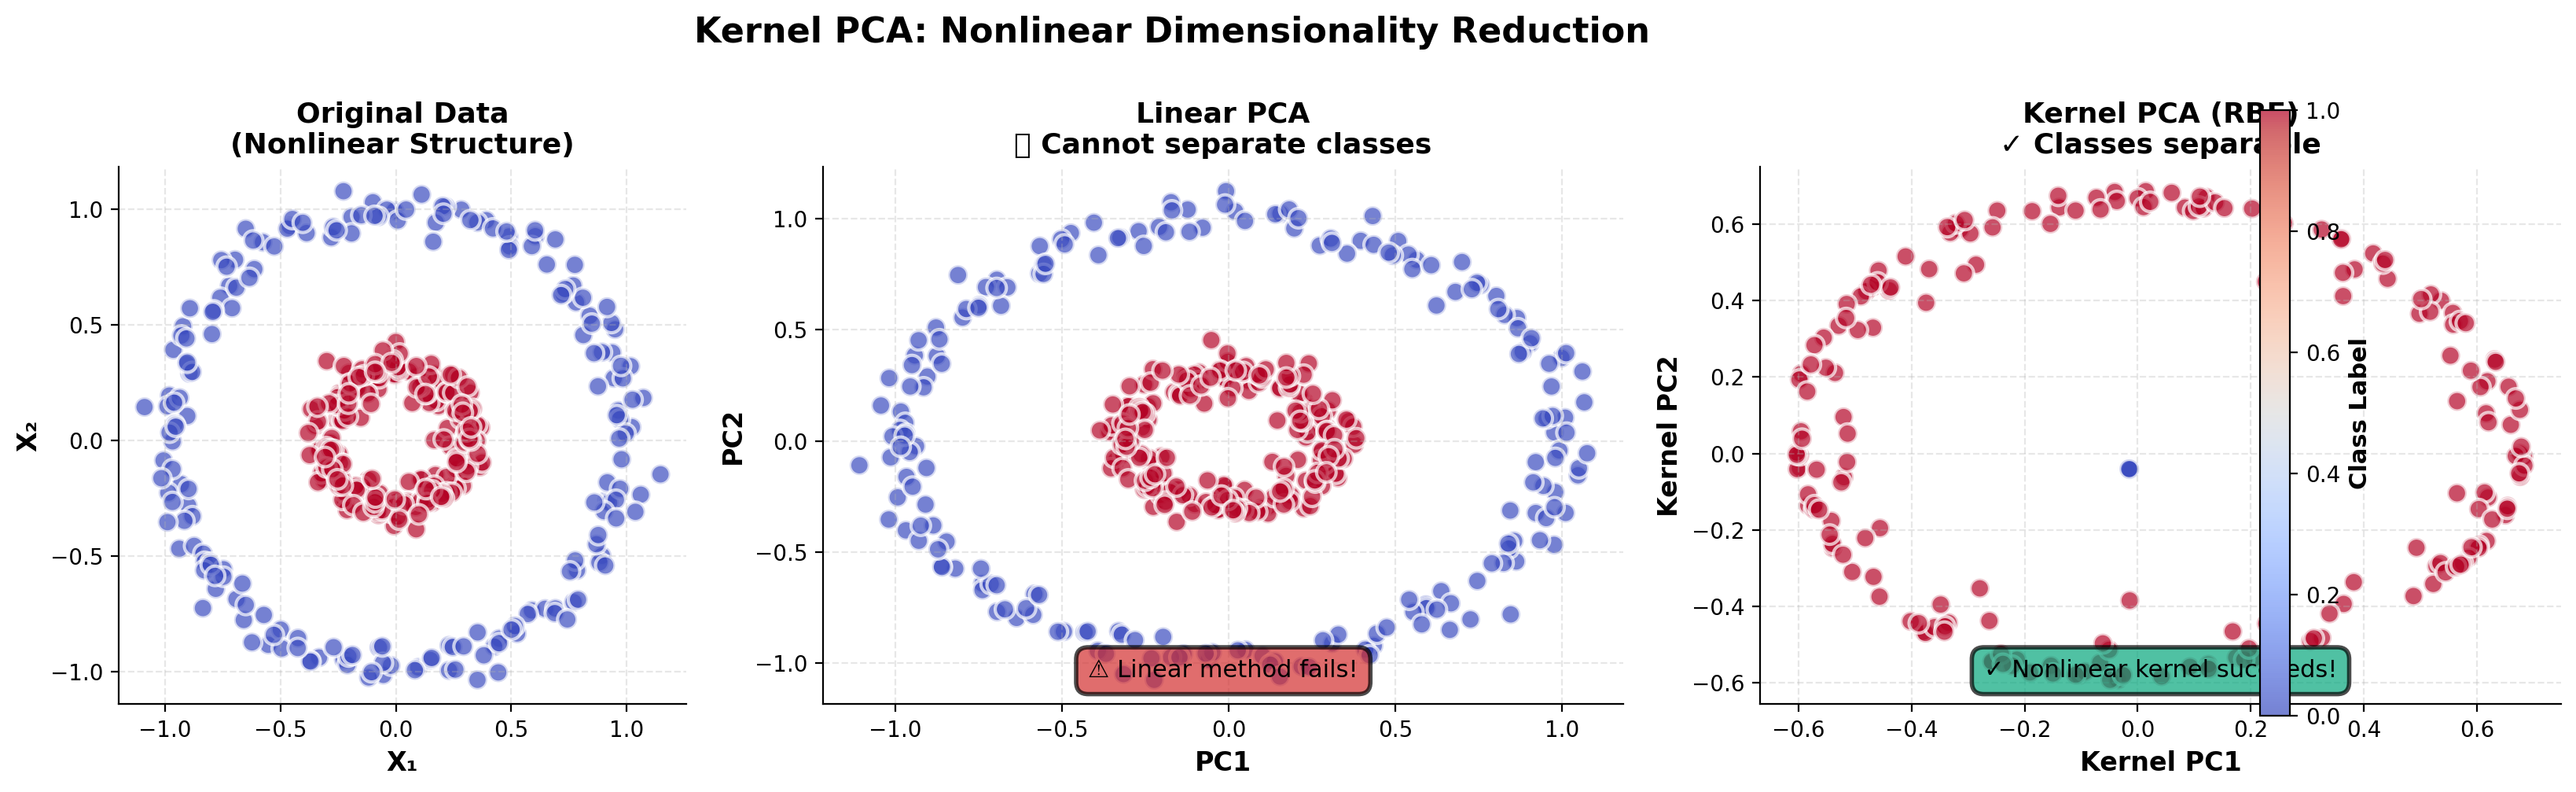
\includegraphics[width=\textwidth]{../figures/kernel_pca_concept.png}

\vspace{0.2cm}

\textbf{Common Kernels:}
\begin{itemize}
\setlength{\itemsep}{2pt}
\item \textbf{RBF:} $K(x,y) = \exp(-\gamma\|x-y\|^2)$
\item \textbf{Polynomial:} $K(x,y) = (x^Ty + c)^d$
\item \textbf{Sigmoid:} $K(x,y) = \tanh(\alpha x^Ty + c)$
\end{itemize}

\vspace{0.2cm}

\begin{exampleblock}{Applications}
\begin{itemize}
\setlength{\itemsep}{0pt}
\item Manifold learning
\item Non-linear dimensionality reduction
\item Feature extraction for non-linear data
\end{itemize}
\end{exampleblock}

\vspace{0.2cm}

\begin{alertblock}{Trade-off}
More flexible but computationally expensive: $\mathcal{O}(n^3)$
\end{alertblock}
\end{column}
\end{columns}
\end{frame}

\begin{frame}{Sparse PCA}
\begin{columns}[t]
\begin{column}{0.48\textwidth}
\begin{block}{Motivation}
Standard PCA produces components that are linear combinations of \textbf{all} original features, making interpretation difficult.
\end{block}

\vspace{0.2cm}

\textbf{Goal:} Find PCs with \textbf{sparse loadings}
\begin{itemize}
\setlength{\itemsep}{2pt}
\item Most loadings are exactly zero
\item Only few features contribute to each PC
\item Easier interpretation
\item Feature selection built-in
\end{itemize}

\vspace{0.2cm}

\textbf{Formulation:}
$$\min_{\mathbf{V}} \|\mathbf{X} - \mathbf{X}\mathbf{V}\mathbf{V}^T\|_F^2 + \lambda\sum_{j=1}^{k}\|\mathbf{v}_j\|_1$$

\vspace{0.2cm}

\begin{itemize}
\setlength{\itemsep}{2pt}
\item First term: Reconstruction error
\item Second term: Sparsity penalty (L1 regularization)
\item $\lambda$: Controls sparsity level
\end{itemize}
\end{column}

\begin{column}{0.48\textwidth}
\centering
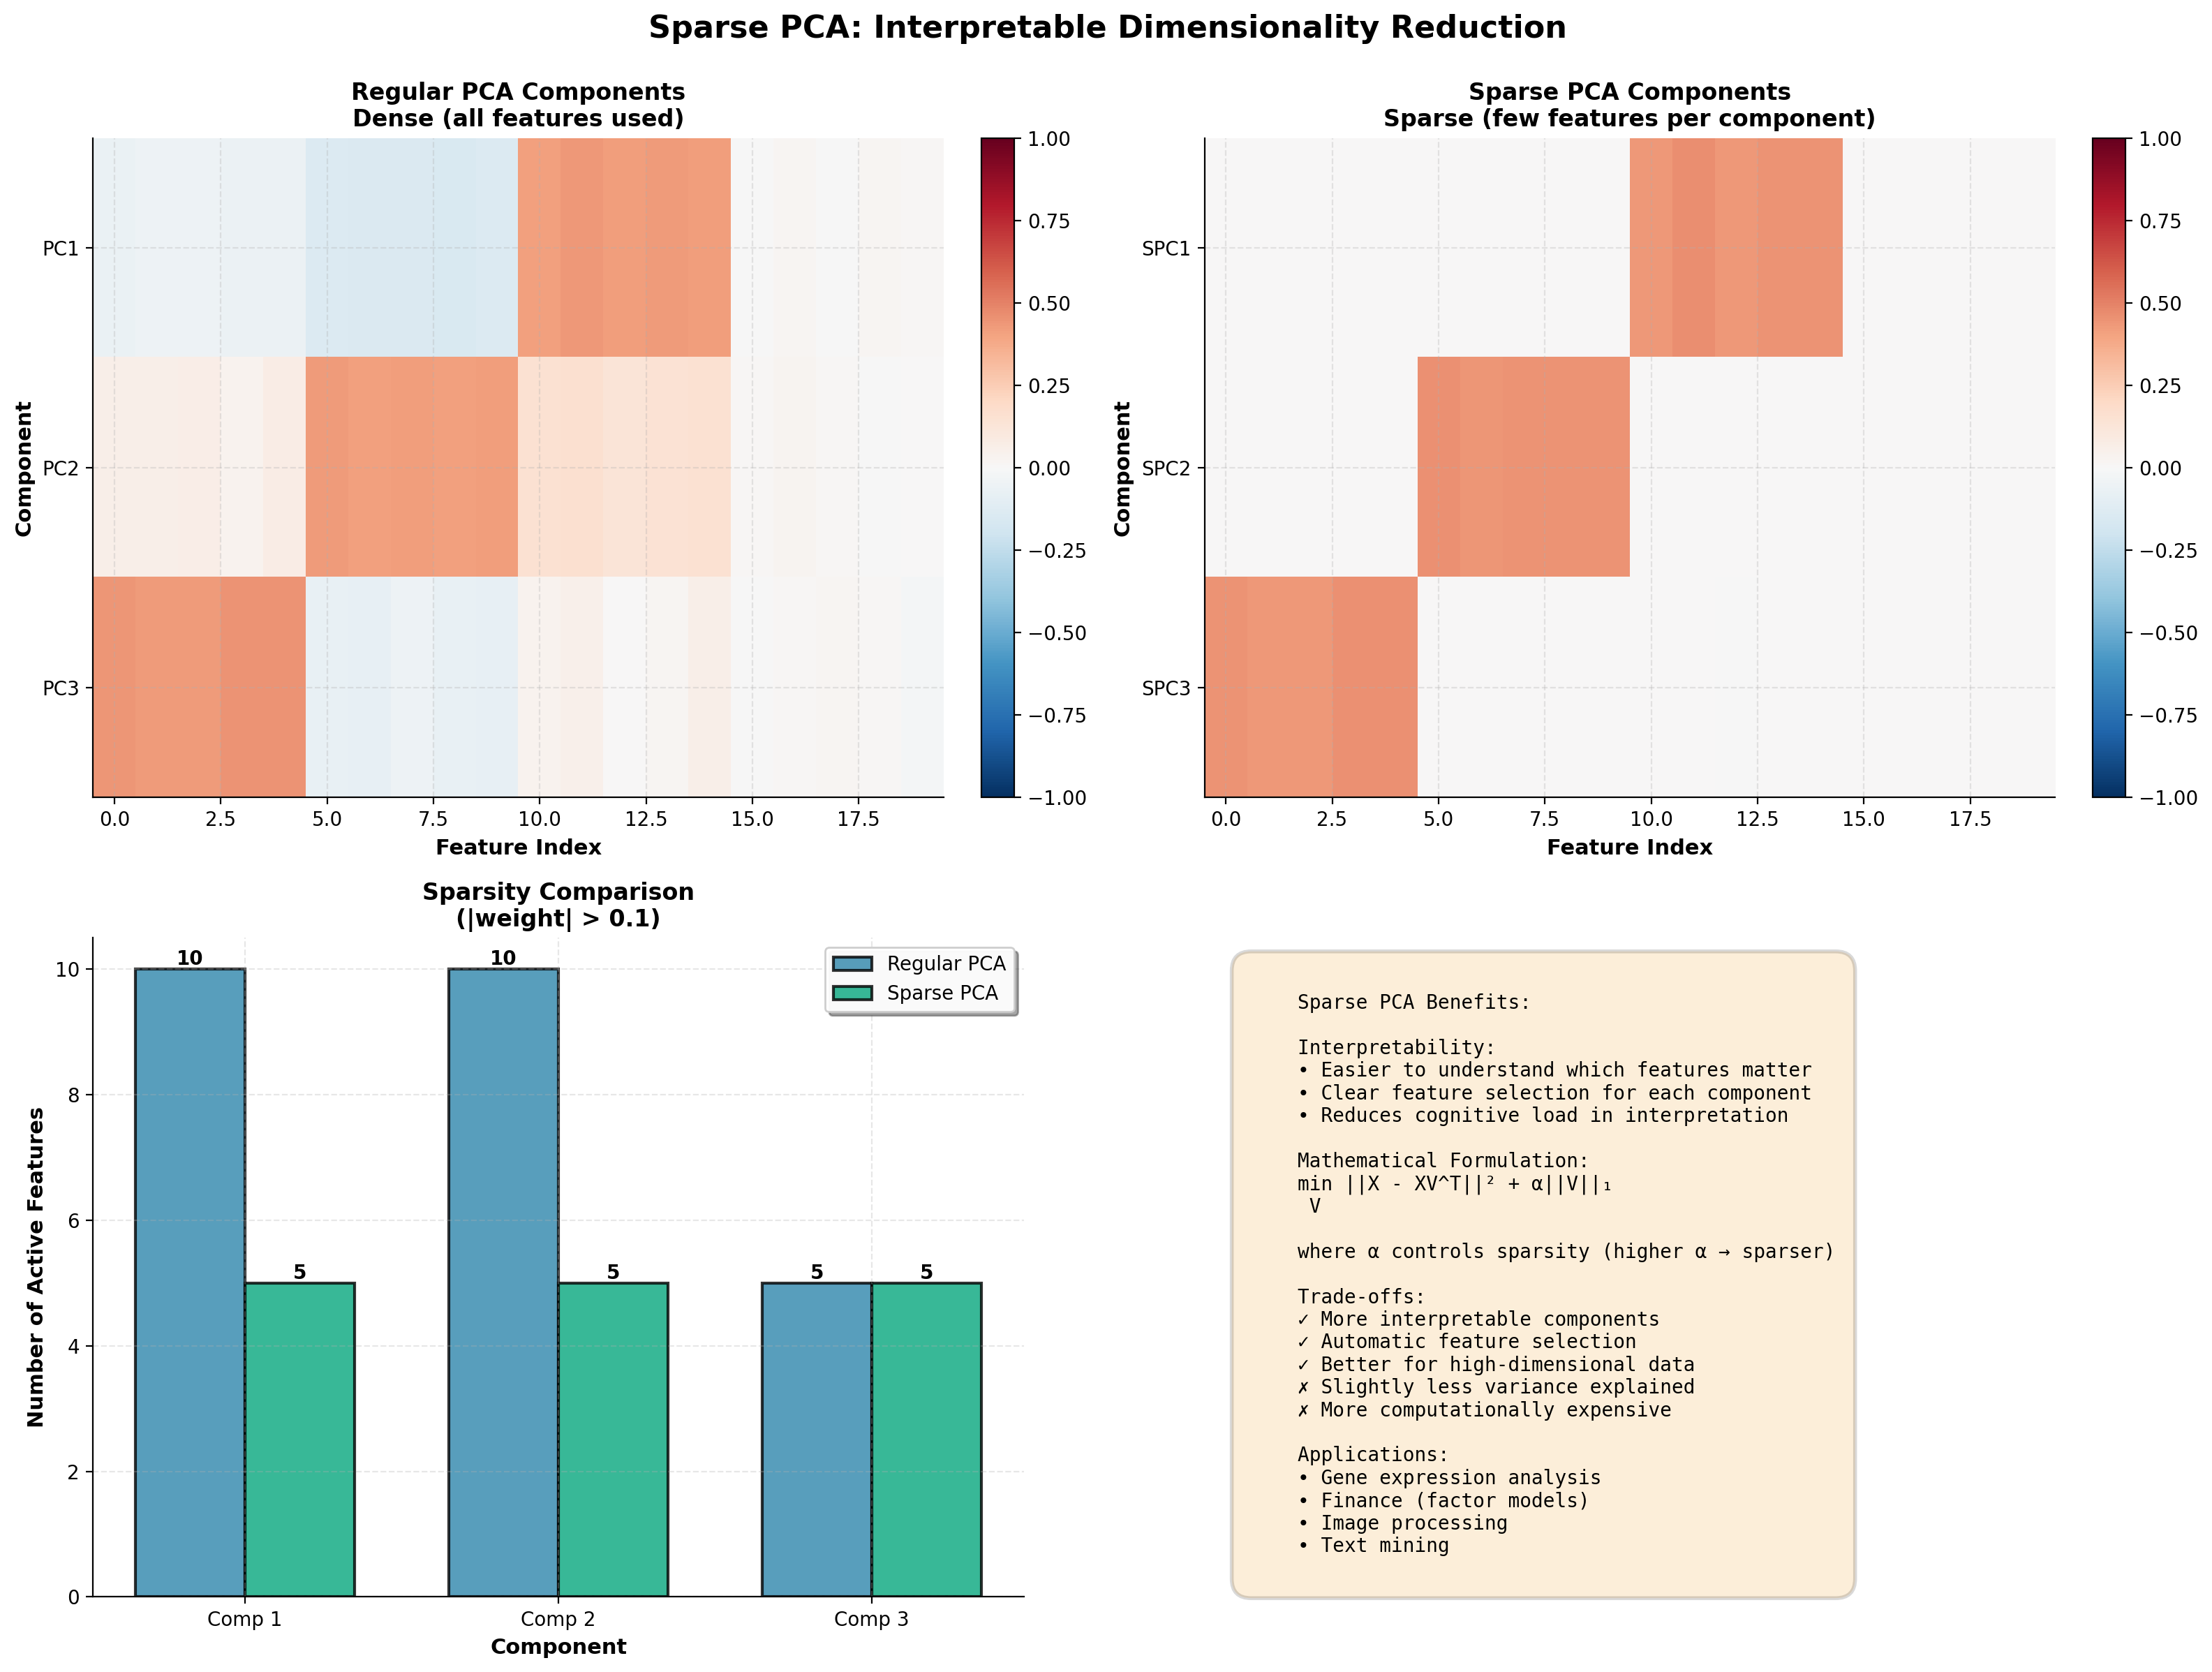
\includegraphics[width=\textwidth]{../figures/sparse_pca.png}

\vspace{0.2cm}

\textbf{Comparison:}

\begin{tabular}{|l|c|c|}
\hline
\textbf{Method} & \textbf{Variance} & \textbf{Sparsity} \\
\hline
Standard PCA & 100\% & 0\% \\
Sparse PCA & 95-98\% & 70-90\% \\
\hline
\end{tabular}

\vspace{0.2cm}

\textbf{Applications:}
\begin{itemize}
\setlength{\itemsep}{2pt}
\item Gene expression analysis
\item Financial data analysis
\item Text mining
\item Any domain requiring interpretability
\end{itemize}

\vspace{0.2cm}

\begin{alertblock}{Trade-off}
Slight loss of explained variance for much better interpretability.
\end{alertblock}
\end{column}
\end{columns}
\end{frame}

\begin{frame}{Incremental PCA}
\begin{columns}[t]
\begin{column}{0.48\textwidth}
\begin{block}{Motivation}
Standard PCA requires entire dataset in memory. Not feasible for:
\begin{itemize}
\setlength{\itemsep}{2pt}
\item Very large datasets
\item Streaming data
\item Online learning scenarios
\item Limited memory systems
\end{itemize}
\end{block}

\vspace{0.2cm}

\textbf{Key Idea:}
Process data in \textbf{mini-batches}:
\begin{enumerate}
\setlength{\itemsep}{2pt}
\item Initialize with first batch
\item Update PCs incrementally with new batches
\item Maintain approximate PCs online
\item Never load full dataset
\end{enumerate}

\vspace{0.2cm}

\textbf{Algorithm Sketch:}
\begin{algorithmic}[1]
\STATE Initialize: $\mathbf{V}_0$, $\mathbf{\Sigma}_0$, $n_0$
\FOR{each batch $\mathbf{X}_b$}
\STATE Update mean: $\bar{\mathbf{x}}_{new}$
\STATE Update covariance: $\mathbf{\Sigma}_{new}$
\STATE SVD: Update $\mathbf{V}$
\STATE $n \gets n + n_b$
\ENDFOR
\end{algorithmic}
\end{column}

\begin{column}{0.48\textwidth}
\centering
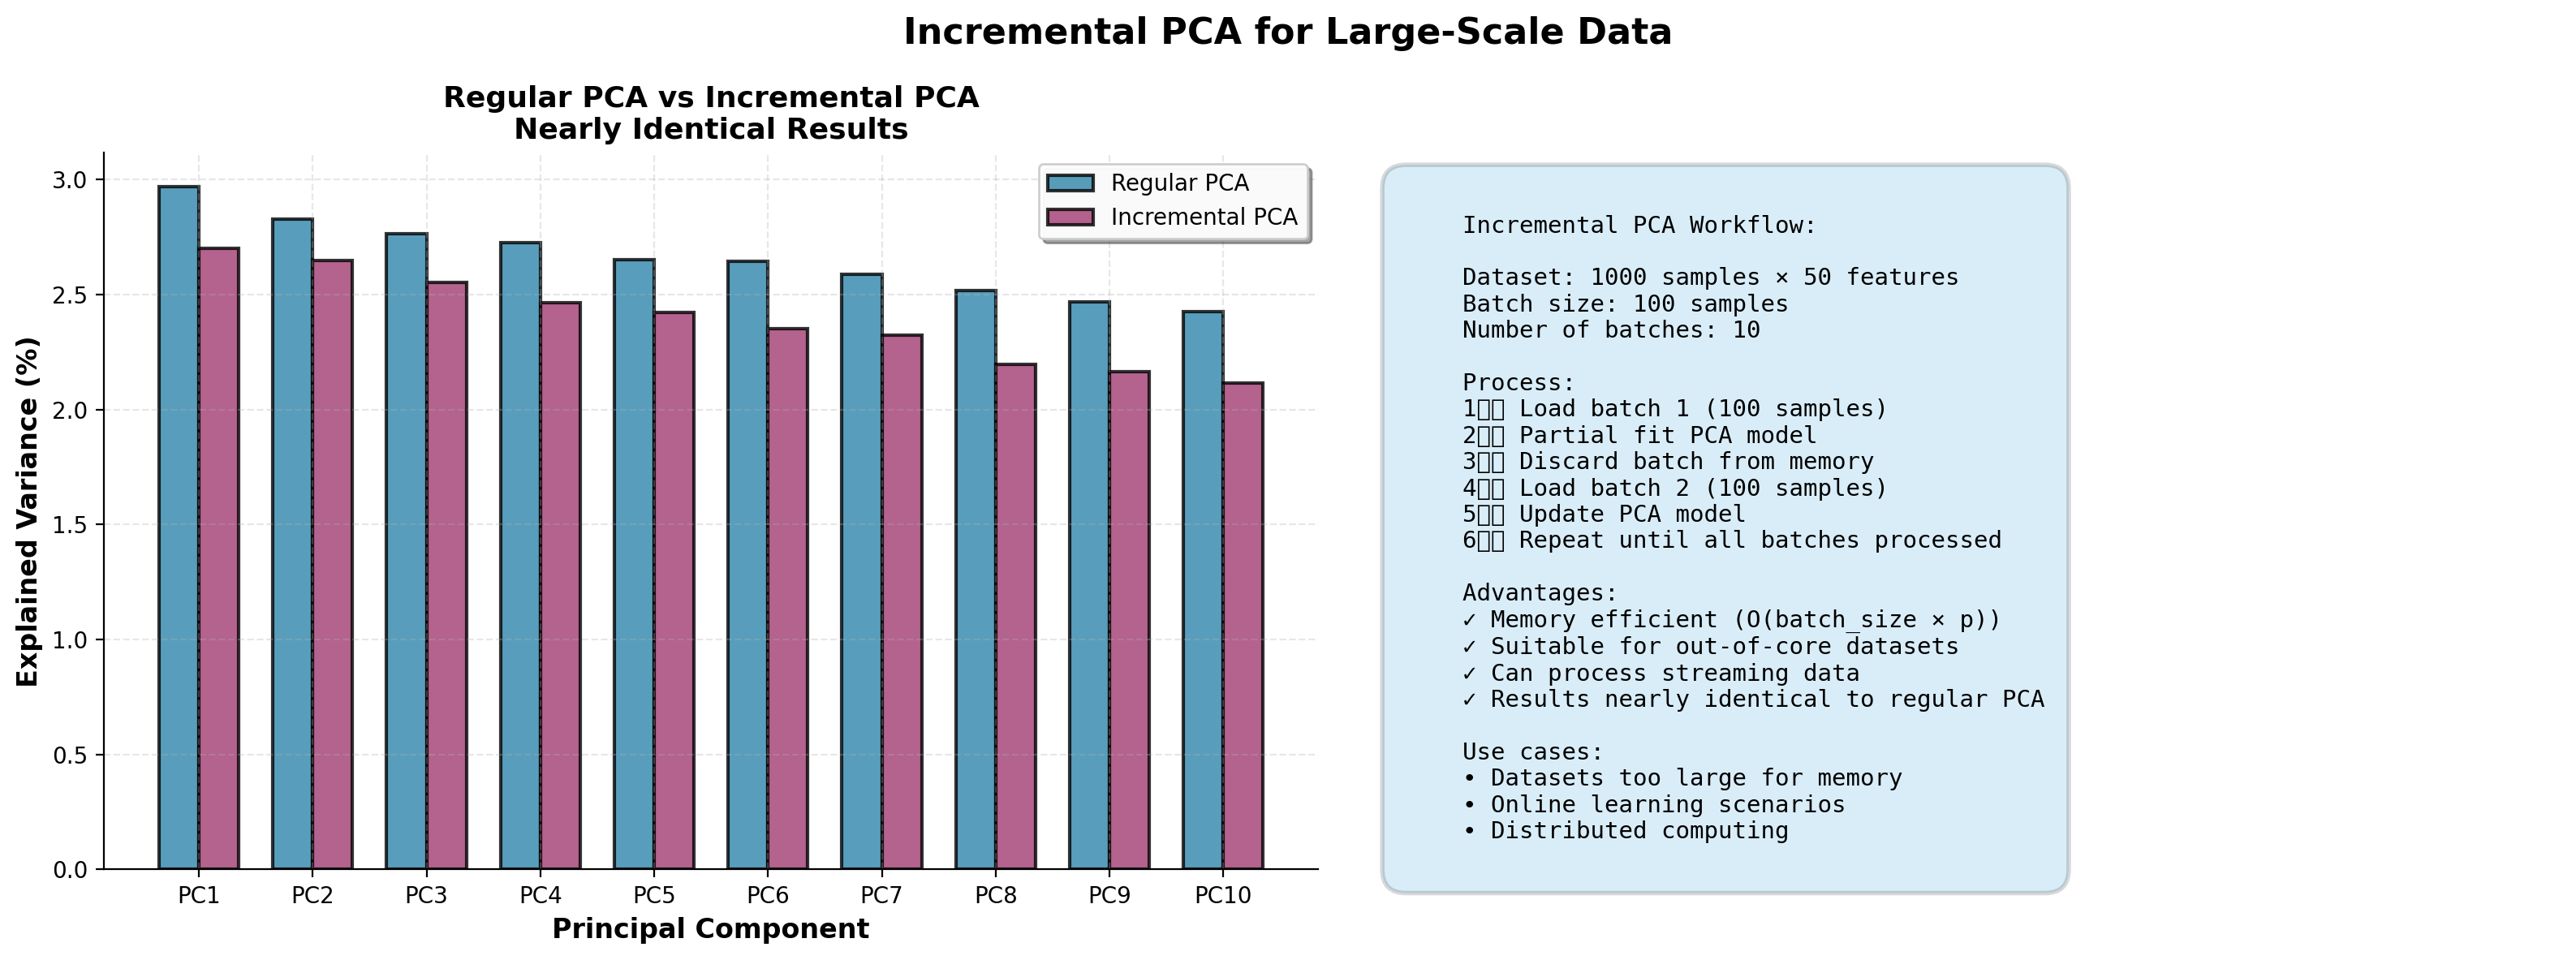
\includegraphics[width=\textwidth]{../figures/incremental_pca.png}

\vspace{0.2cm}

\textbf{Advantages:}
\begin{itemize}
\setlength{\itemsep}{2pt}
\item \textcolor{blue}{Memory efficient}: Constant memory
\item \textcolor{green}{Scalable}: Handles large data
\item \textcolor{purple}{Online}: Updates with new data
\item \textcolor{red}{Streaming}: Real-time processing
\end{itemize}

\vspace{0.2cm}

\textbf{Complexity:}
\begin{itemize}
\setlength{\itemsep}{2pt}
\item Per batch: $\mathcal{O}(bd^2)$ where $b$ = batch size
\item Memory: $\mathcal{O}(d^2)$ instead of $\mathcal{O}(nd)$
\item Nearly identical results to batch PCA
\end{itemize}

\vspace{0.2cm}

\begin{exampleblock}{Use Cases}
\begin{itemize}
\setlength{\itemsep}{0pt}
\item Large-scale image processing
\item Sensor data streams
\item Online recommendation systems
\end{itemize}
\end{exampleblock}
\end{column}
\end{columns}
\end{frame}

\begin{frame}{Probabilistic PCA}
\begin{columns}[t]
\begin{column}{0.48\textwidth}
\begin{block}{Motivation}
Standard PCA is deterministic. Probabilistic PCA provides:
\begin{itemize}
\setlength{\itemsep}{2pt}
\item Generative model of data
\item Handling of missing values
\item Uncertainty quantification
\item Bayesian extensions
\end{itemize}
\end{block}

\vspace{0.2cm}

\textbf{Model:}
\begin{align}
\mathbf{z} &\sim \mathcal{N}(0, \mathbf{I}_k) \\
\mathbf{x}|\mathbf{z} &\sim \mathcal{N}(\mathbf{W}\mathbf{z} + \boldsymbol{\mu}, \sigma^2\mathbf{I}_d)
\end{align}

where:
\begin{itemize}
\setlength{\itemsep}{0pt}
\item $\mathbf{z} \in \mathbb{R}^k$: Latent variables
\item $\mathbf{W} \in \mathbb{R}^{d \times k}$: Loading matrix
\item $\sigma^2$: Isotropic noise
\end{itemize}

\vspace{0.2cm}

\textbf{Maximum Likelihood Solution:}
$$\mathbf{W}_{ML} = \mathbf{V}_k(\mathbf{\Lambda}_k - \sigma^2\mathbf{I})^{1/2}\mathbf{R}$$

where $\mathbf{R}$ is arbitrary rotation.
\end{column}

\begin{column}{0.48\textwidth}
\textbf{EM Algorithm:}

\begin{algorithmic}[1]
\STATE Initialize $\mathbf{W}$, $\sigma^2$
\REPEAT
\STATE \textbf{E-step:} Compute $\mathbb{E}[\mathbf{z}|\mathbf{x}]$
\STATE \textbf{M-step:} Update $\mathbf{W}$, $\sigma^2$
\UNTIL{convergence}
\end{algorithmic}

\vspace{0.2cm}

\textbf{Advantages:}
\begin{itemize}
\setlength{\itemsep}{2pt}
\item Handle missing data naturally
\item Mixture of PPCAs for clustering
\item Bayesian inference possible
\item Uncertainty quantification
\end{itemize}

\vspace{0.2cm}

\textbf{Relationship to Standard PCA:}
\begin{itemize}
\setlength{\itemsep}{2pt}
\item As $\sigma^2 \to 0$: Recovers standard PCA
\item Same subspace in limit
\item Additional noise model
\end{itemize}

\vspace{0.2cm}

\begin{exampleblock}{Extensions}
\begin{itemize}
\setlength{\itemsep}{0pt}
\item Factor Analysis: Non-isotropic noise
\item Variational PCA: Variational inference
\item Sparse PPCA: Sparse loadings
\end{itemize}
\end{exampleblock}
\end{column}
\end{columns}
\end{frame}

\begin{frame}{Robust PCA}
\begin{columns}[t]
\begin{column}{0.48\textwidth}
\begin{block}{Motivation}
Standard PCA is sensitive to:
\begin{itemize}
\setlength{\itemsep}{2pt}
\item Outliers: Anomalous data points
\item Corrupted entries: Missing or noisy values
\item Sparse errors: Localized corruption
\end{itemize}
\end{block}

\vspace{0.2cm}

\textbf{Problem Formulation:}

Decompose $\mathbf{X}$ into:
$$\mathbf{X} = \mathbf{L} + \mathbf{S}$$

where:
\begin{itemize}
\setlength{\itemsep}{2pt}
\item $\mathbf{L}$: Low-rank (clean data)
\item $\mathbf{S}$: Sparse (outliers/corruption)
\end{itemize}

\vspace{0.2cm}

\textbf{Optimization:}
$$\min_{\mathbf{L},\mathbf{S}} \|\mathbf{L}\|_* + \lambda\|\mathbf{S}\|_1$$
$$\text{subject to } \mathbf{X} = \mathbf{L} + \mathbf{S}$$

\begin{itemize}
\setlength{\itemsep}{0pt}
\item $\|\mathbf{L}\|_*$: Nuclear norm (rank proxy)
\item $\|\mathbf{S}\|_1$: L1 norm (sparsity)
\end{itemize}
\end{column}

\begin{column}{0.48\textwidth}
\textbf{Applications:}

\vspace{0.2cm}

\begin{exampleblock}{Video Surveillance}
\begin{itemize}
\setlength{\itemsep}{0pt}
\item $\mathbf{L}$: Static background
\item $\mathbf{S}$: Moving objects
\item Separates foreground/background
\end{itemize}
\end{exampleblock}

\vspace{0.2cm}

\begin{exampleblock}{Face Recognition}
\begin{itemize}
\setlength{\itemsep}{0pt}
\item $\mathbf{L}$: Face structure
\item $\mathbf{S}$: Occlusions, shadows
\item Robust to partial occlusion
\end{itemize}
\end{exampleblock}

\vspace{0.2cm}

\textbf{Solution Methods:}
\begin{itemize}
\setlength{\itemsep}{2pt}
\item Principal Component Pursuit (PCP)
\item Alternating Direction Method (ADMM)
\item Proximal gradient methods
\end{itemize}

\vspace{0.2cm}

\textbf{Complexity:}
\begin{itemize}
\setlength{\itemsep}{2pt}
\item $\mathcal{O}(nd^2k)$ per iteration
\item Slower than standard PCA
\item Worth it for corrupted data
\end{itemize}
\end{column}
\end{columns}
\end{frame}

% ========================================
% Section: Evaluation & Selection
% ========================================

\section{Evaluation \& Component Selection}

\begin{frame}{Scree Plot: Visualizing Variance}
\begin{columns}[t]
\begin{column}{0.48\textwidth}
\begin{block}{Definition}
A \textbf{scree plot} displays eigenvalues (or explained variance) for each principal component in decreasing order.
\end{block}

\vspace{0.2cm}

\textbf{How to Read:}
\begin{itemize}
\setlength{\itemsep}{2pt}
\item X-axis: Principal component number
\item Y-axis: Eigenvalue or explained variance
\item Look for "elbow" point
\item Steep drop indicates important PCs
\item Flat tail indicates noise
\end{itemize}

\vspace{0.2cm}

\textbf{Elbow Method:}
\begin{itemize}
\setlength{\itemsep}{2pt}
\item Find point where curve bends
\item Keep PCs before elbow
\item Remaining PCs contribute little
\item Subjective but practical
\end{itemize}

\vspace{0.2cm}

\begin{alertblock}{Rule of Thumb}
Keep components before the "elbow" where variance drops sharply.
\end{alertblock}
\end{column}

\begin{column}{0.48\textwidth}
\centering
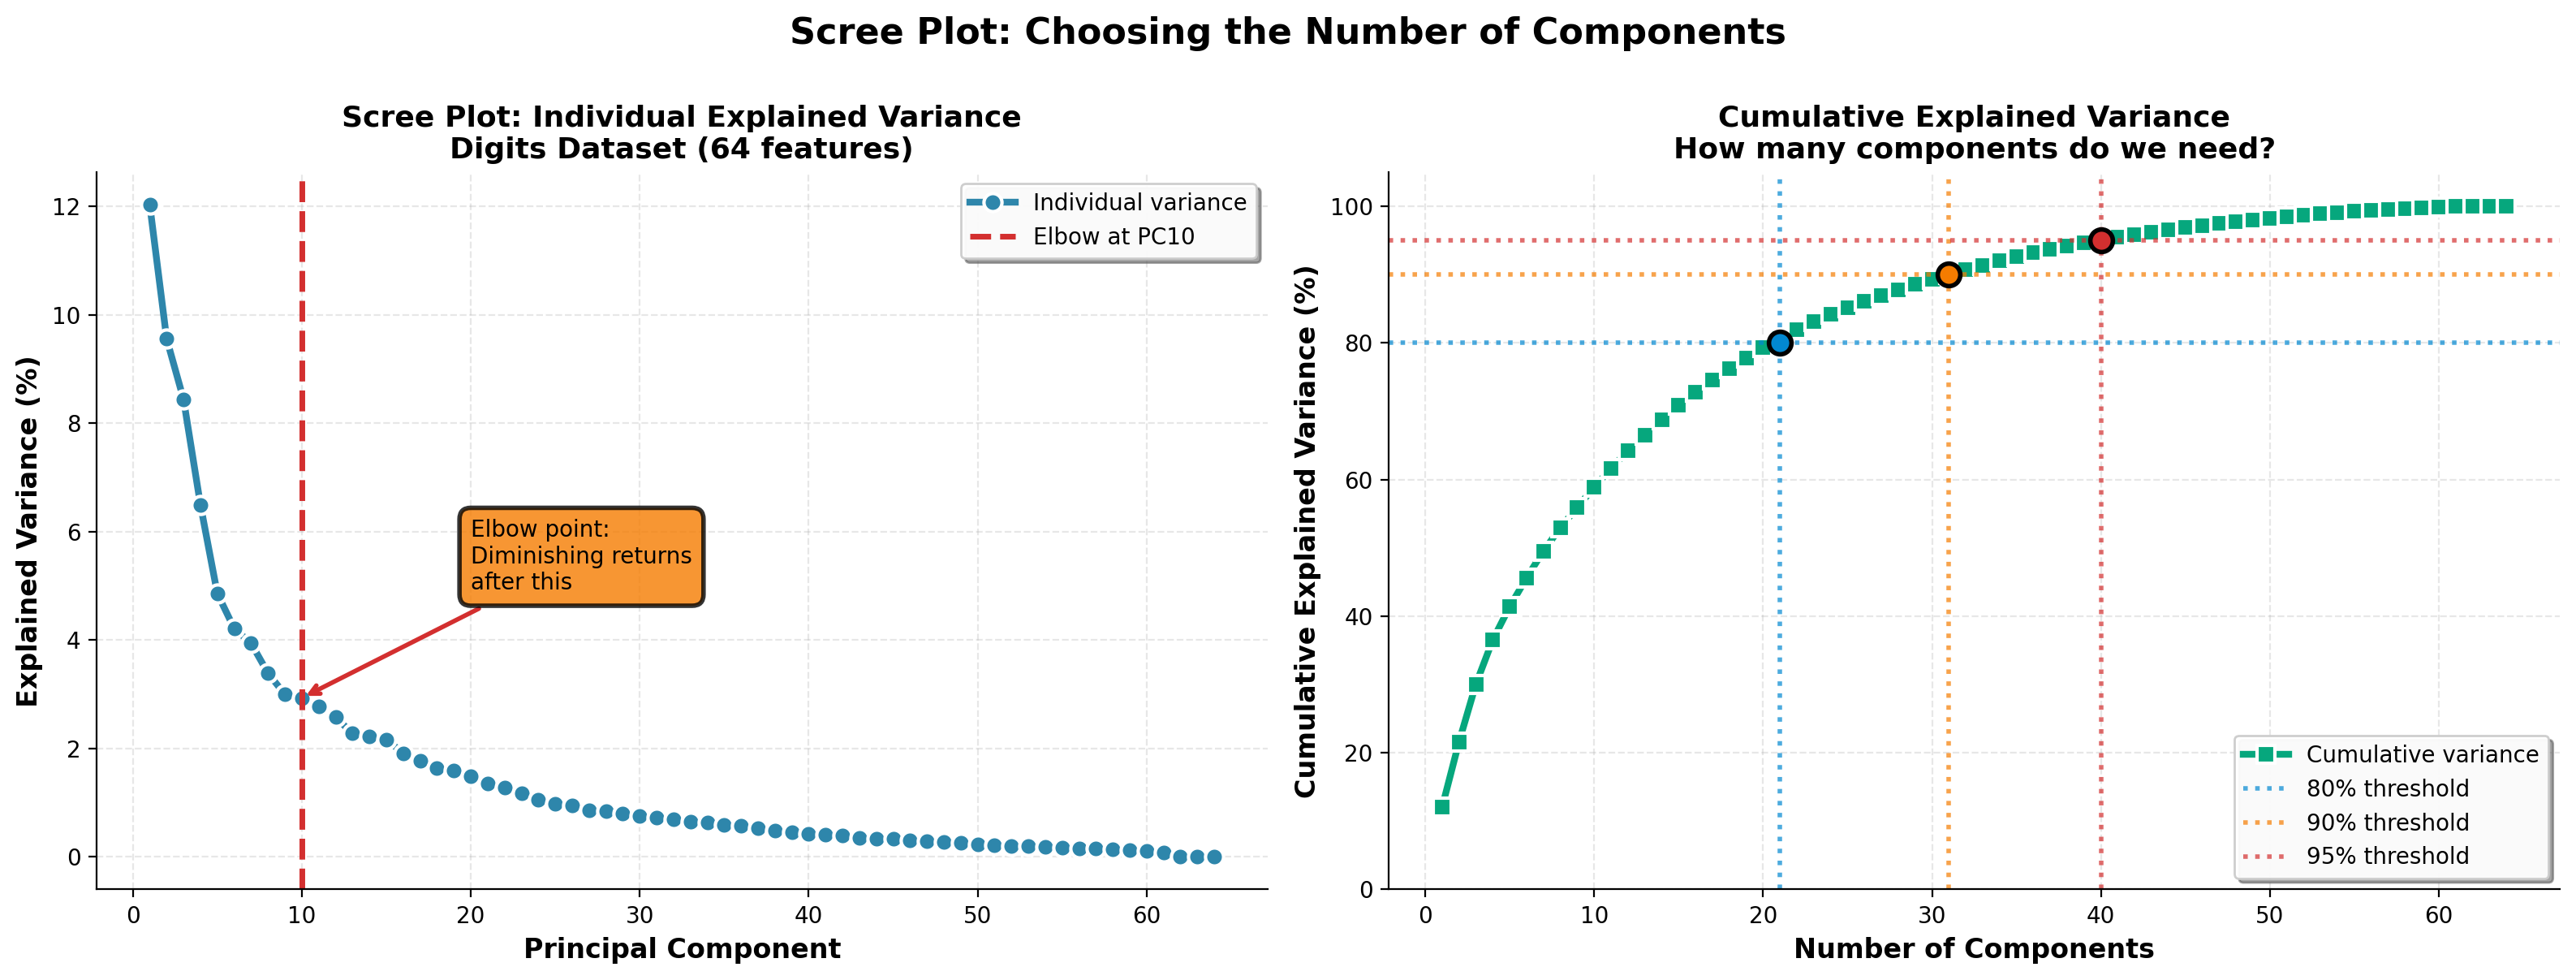
\includegraphics[width=\textwidth]{../figures/scree_plot.png}

\vspace{0.2cm}

\textbf{Example Interpretation:}
\begin{itemize}
\setlength{\itemsep}{2pt}
\item PC1: Large eigenvalue (most variance)
\item PC2-3: Moderate decrease
\item PC4+: Flat (noise level)
\item \textbf{Decision:} Keep 3-4 components
\end{itemize}

\vspace{0.2cm}

\begin{exampleblock}{Kaiser Criterion}
Alternative rule: Keep components with eigenvalue $> 1$ (for correlation matrix).
\end{exampleblock}
\end{column}
\end{columns}
\end{frame}

\begin{frame}{Explained Variance Ratio}
\begin{columns}[t]
\begin{column}{0.48\textwidth}
\textbf{Individual Explained Variance:}

For component $i$:
$$\text{EVR}_i = \frac{\lambda_i}{\sum_{j=1}^{d}\lambda_j}$$

\vspace{0.2cm}

\textbf{Cumulative Explained Variance:}

For first $k$ components:
$$\text{CEV}_k = \frac{\sum_{i=1}^{k}\lambda_i}{\sum_{j=1}^{d}\lambda_j}$$

\vspace{0.2cm}

\textbf{Selection Criteria:}
\begin{itemize}
\setlength{\itemsep}{2pt}
\item \textbf{Fixed threshold:} $\text{CEV}_k \geq 0.95$ (95\%)
\item \textbf{Fixed number:} $k = 10$ components
\item \textbf{Elbow method:} Visual inspection
\item \textbf{Cross-validation:} Best downstream performance
\end{itemize}

\vspace{0.2cm}

\begin{alertblock}{Common Choice}
Keep components explaining 90-95\% of total variance.
\end{alertblock}
\end{column}

\begin{column}{0.48\textwidth}
\textbf{Example Calculation:}

Eigenvalues: $[5.2, 2.1, 0.8, 0.3, 0.1]$

Total: $\sum \lambda_i = 8.5$

\vspace{0.2cm}

\begin{tabular}{|c|c|c|}
\hline
\textbf{PC} & \textbf{EVR} & \textbf{CEV} \\
\hline
1 & 61.2\% & 61.2\% \\
2 & 24.7\% & 85.9\% \\
3 & 9.4\% & 95.3\% \\
4 & 3.5\% & 98.8\% \\
5 & 1.2\% & 100.0\% \\
\hline
\end{tabular}

\vspace{0.2cm}

\textbf{Decision:}
\begin{itemize}
\setlength{\itemsep}{2pt}
\item For 85\% variance: Keep 2 PCs
\item For 95\% variance: Keep 3 PCs
\item For 99\% variance: Keep 4 PCs
\end{itemize}

\vspace{0.2cm}

\begin{exampleblock}{Trade-off}
More components: Better reconstruction, less compression
\end{exampleblock}
\end{column}
\end{columns}
\end{frame}

\begin{frame}{Reconstruction Error}
\begin{columns}[t]
\begin{column}{0.48\textwidth}
\begin{block}{Definition}
\textbf{Reconstruction error} measures information lost when using only $k < d$ principal components.
\end{block}

\vspace{0.2cm}

\textbf{Formula:}
$$E_k = \|\mathbf{X} - \hat{\mathbf{X}}_k\|_F^2 = \sum_{i=k+1}^{d}\lambda_i$$

where $\hat{\mathbf{X}}_k = \mathbf{X}\mathbf{V}_k\mathbf{V}_k^T$

\vspace{0.2cm}

\textbf{Normalized Error:}
$$\text{Relative Error} = \frac{E_k}{\|\mathbf{X}\|_F^2} = \frac{\sum_{i=k+1}^{d}\lambda_i}{\sum_{i=1}^{d}\lambda_i}$$

\vspace{0.2cm}

\textbf{Properties:}
\begin{itemize}
\setlength{\itemsep}{2pt}
\item Monotonically decreasing in $k$
\item Zero when $k = d$ (perfect reconstruction)
\item Directly related to discarded eigenvalues
\end{itemize}
\end{column}

\begin{column}{0.48\textwidth}
\centering
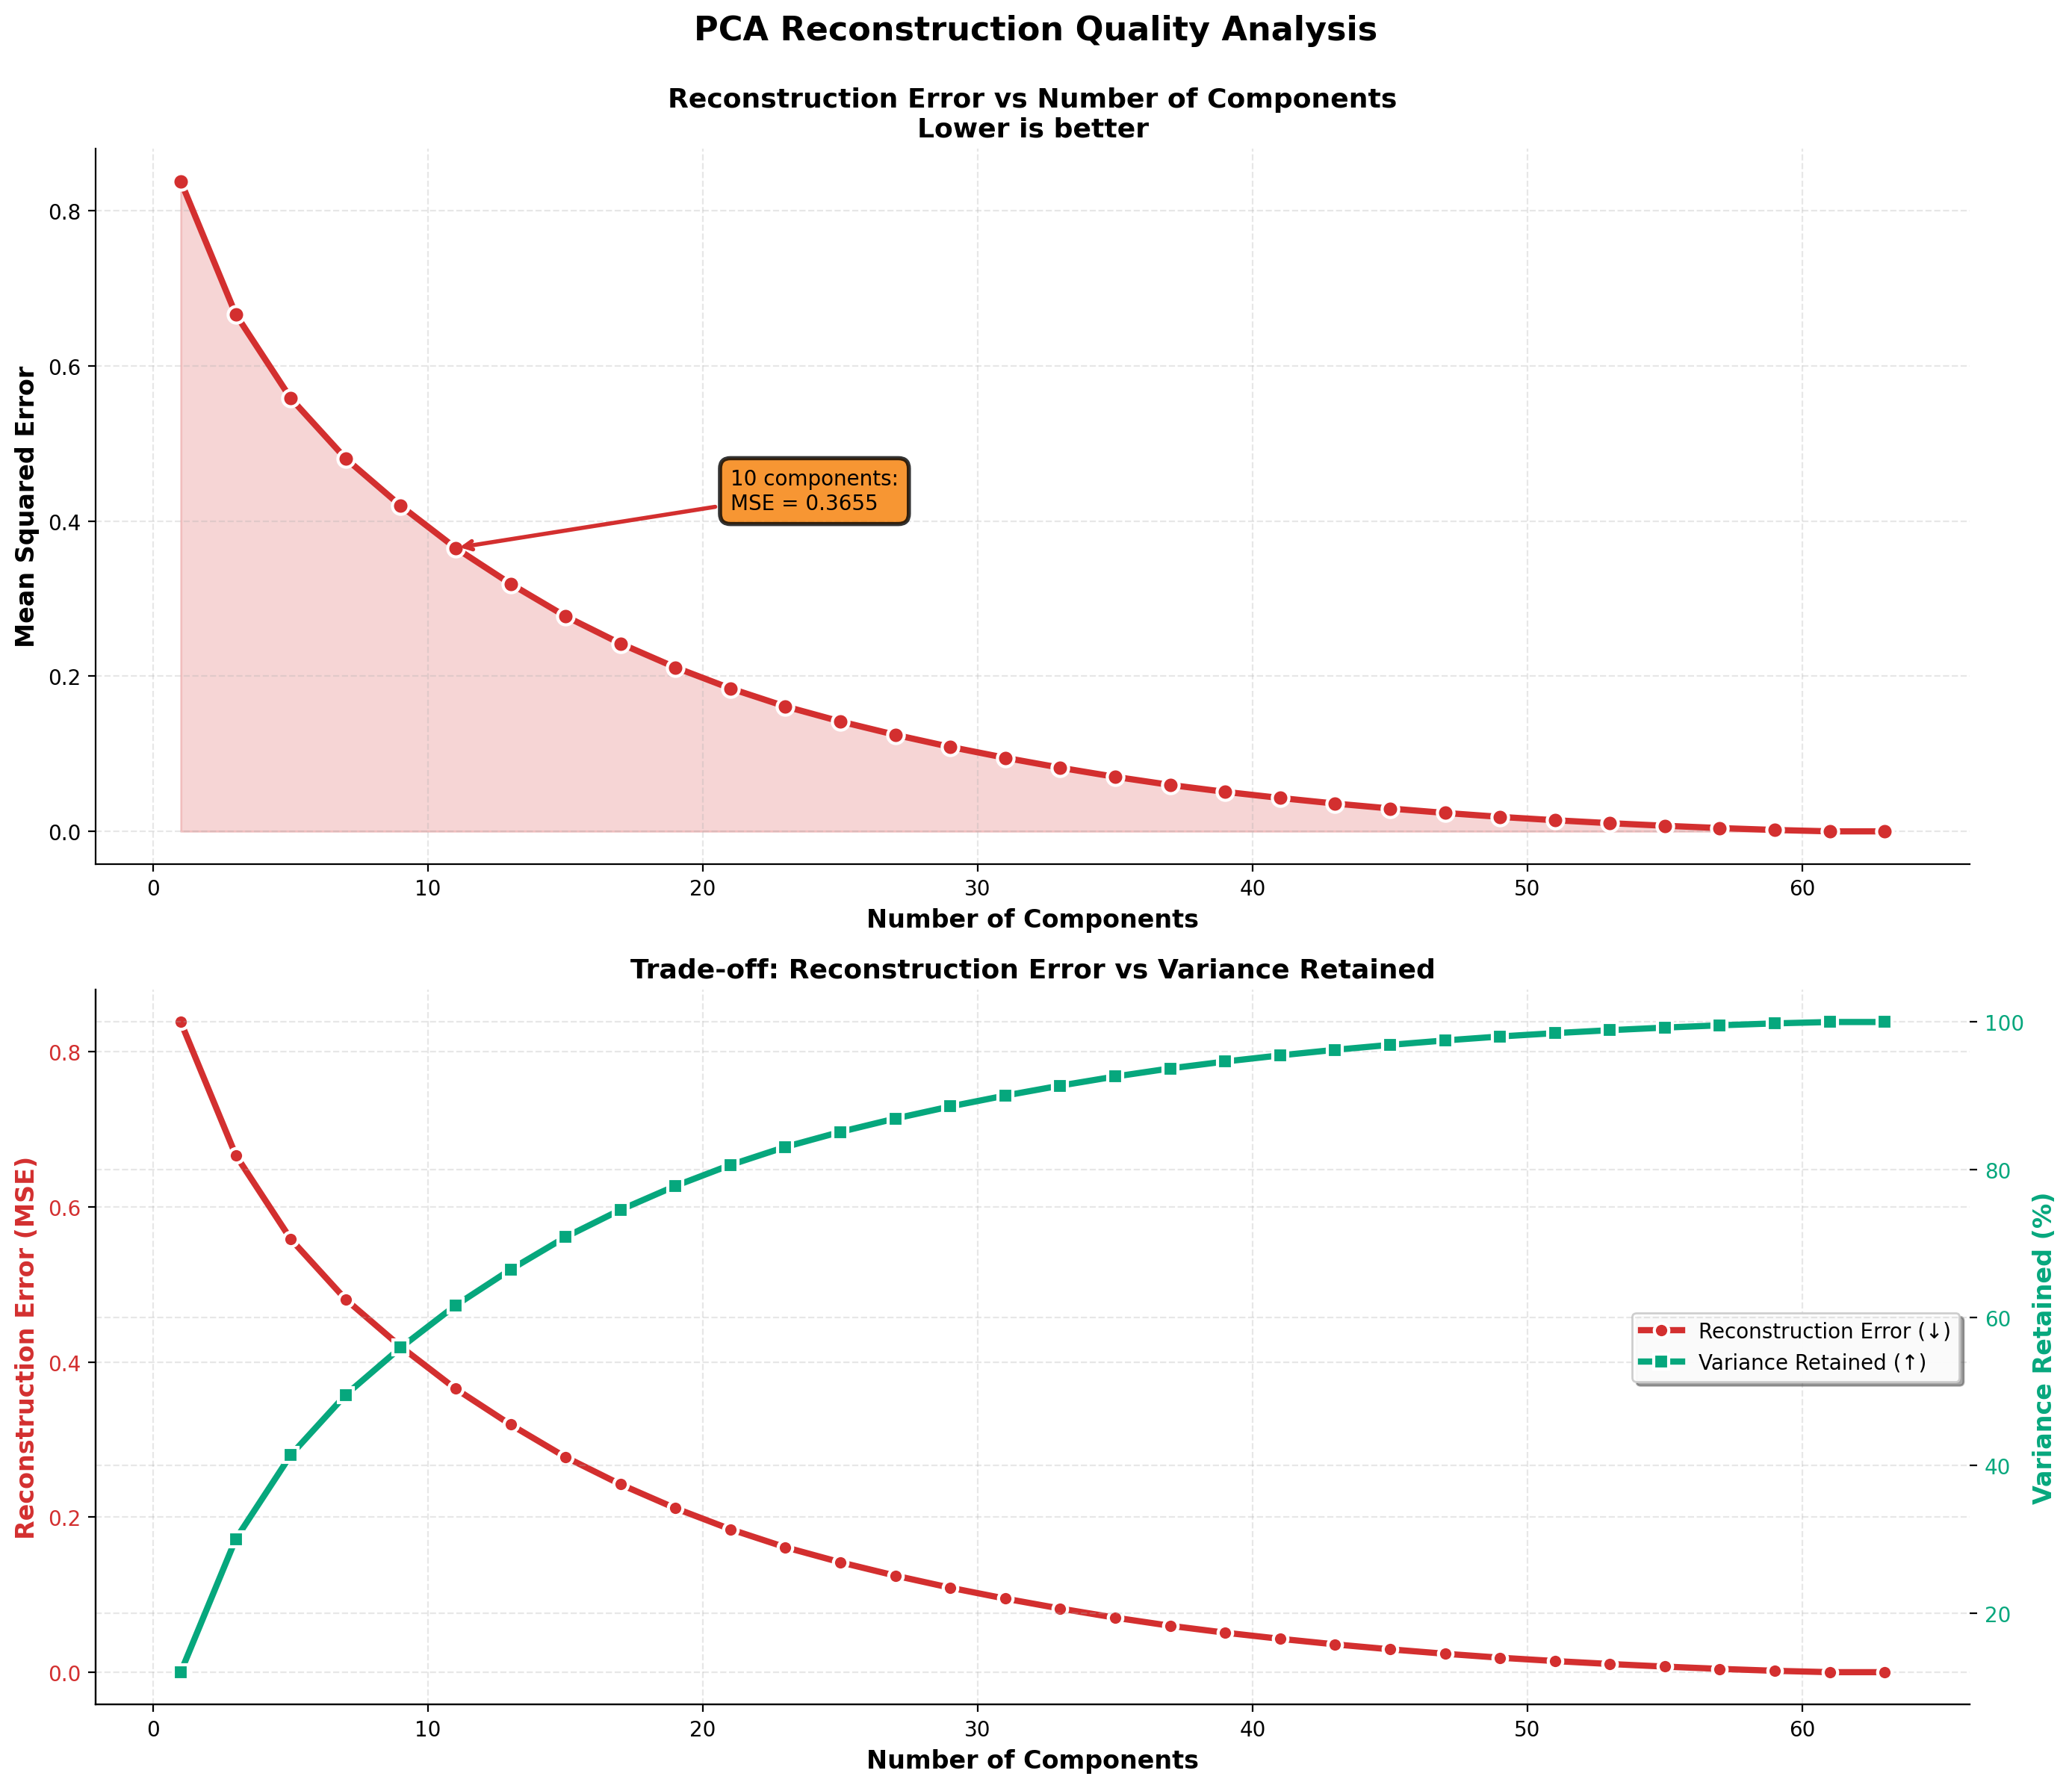
\includegraphics[width=\textwidth]{../figures/reconstruction_error.png}

\vspace{0.2cm}

\textbf{Selection Strategy:}

Set error tolerance $\epsilon$:
$$E_k \leq \epsilon \cdot \|\mathbf{X}\|_F^2$$

Choose smallest $k$ satisfying constraint.

\vspace{0.2cm}

\textbf{Example:}
\begin{itemize}
\setlength{\itemsep}{2pt}
\item Total variance: 100
\item Target: 5\% error tolerance
\item Need: CEV $\geq$ 95\%
\item $\sum_{i=1}^{k}\lambda_i \geq 95$
\end{itemize}

\vspace{0.2cm}

\begin{exampleblock}{Application}
Image compression: Balance file size vs quality using reconstruction error.
\end{exampleblock}
\end{column}
\end{columns}
\end{frame}

\begin{frame}{Cross-Validation for Component Selection}
\begin{columns}[t]
\begin{column}{0.48\textwidth}
\textbf{Task-Specific Selection:}

When PCA is used for downstream task:
\begin{enumerate}
\setlength{\itemsep}{2pt}
\item Apply PCA with different $k$ values
\item Train model on reduced data
\item Evaluate on validation set
\item Choose $k$ with best performance
\end{enumerate}

\vspace{0.2cm}

\textbf{Procedure:}
\begin{algorithmic}[1]
\STATE Split data: Train/Validation
\FOR{$k = 1$ to $k_{max}$}
\STATE Fit PCA on training set
\STATE Transform train \& validation
\STATE Train classifier/regressor
\STATE Evaluate performance
\ENDFOR
\STATE Select $k$ with best validation score
\end{algorithmic}

\vspace{0.2cm}

\begin{alertblock}{Important}
Fit PCA only on training data to avoid data leakage!
\end{alertblock}
\end{column}

\begin{column}{0.48\textwidth}
\textbf{Example: Classification Task}

\begin{center}
\begin{tabular}{|c|c|c|}
\hline
\textbf{k} & \textbf{Train Acc} & \textbf{Val Acc} \\
\hline
5 & 0.75 & 0.72 \\
10 & 0.82 & 0.79 \\
20 & 0.89 & 0.85 \\
50 & 0.95 & 0.84 \\
100 & 0.98 & 0.82 \\
\hline
\end{tabular}
\end{center}

\textbf{Analysis:}
\begin{itemize}
\setlength{\itemsep}{2pt}
\item Best validation: $k = 20$
\item $k = 50, 100$: Overfitting
\item Task-specific optimum
\end{itemize}

\vspace{0.2cm}

\textbf{Considerations:}
\begin{itemize}
\setlength{\itemsep}{2pt}
\item Variance explained vs task performance
\item Computational cost
\item Interpretability needs
\item Domain constraints
\end{itemize}

\vspace{0.2cm}

\begin{exampleblock}{Best Practice}
Use cross-validation when PCA is preprocessing step for supervised learning.
\end{exampleblock}
\end{column}
\end{columns}
\end{frame}

\begin{frame}{Component Correlation Analysis}
\begin{columns}[t]
\begin{column}{0.48\textwidth}
\textbf{Goal:} Understand relationships between original features and principal components.

\vspace{0.2cm}

\textbf{Loading Matrix:}

$$\mathbf{V} = [\mathbf{v}_1, \mathbf{v}_2, \ldots, \mathbf{v}_d]$$

\vspace{0.2cm}

\textbf{Interpretation:}
\begin{itemize}
\setlength{\itemsep}{2pt}
\item $v_{ij}$: Contribution of feature $j$ to PC $i$
\item Large $|v_{ij}|$: Feature $j$ important for PC $i$
\item Sign indicates direction of contribution
\item Loadings are correlations (if standardized)
\end{itemize}

\vspace{0.2cm}

\textbf{Biplot:}
\begin{itemize}
\setlength{\itemsep}{2pt}
\item Visualize data and loadings together
\item Arrow length: Variable importance
\item Arrow direction: Correlation with PCs
\item Angle between arrows: Variable correlation
\end{itemize}

\vspace{0.2cm}

\begin{alertblock}{Interpretation}
Close to parallel arrows indicate highly correlated variables.
\end{alertblock}
\end{column}

\begin{column}{0.48\textwidth}
\centering
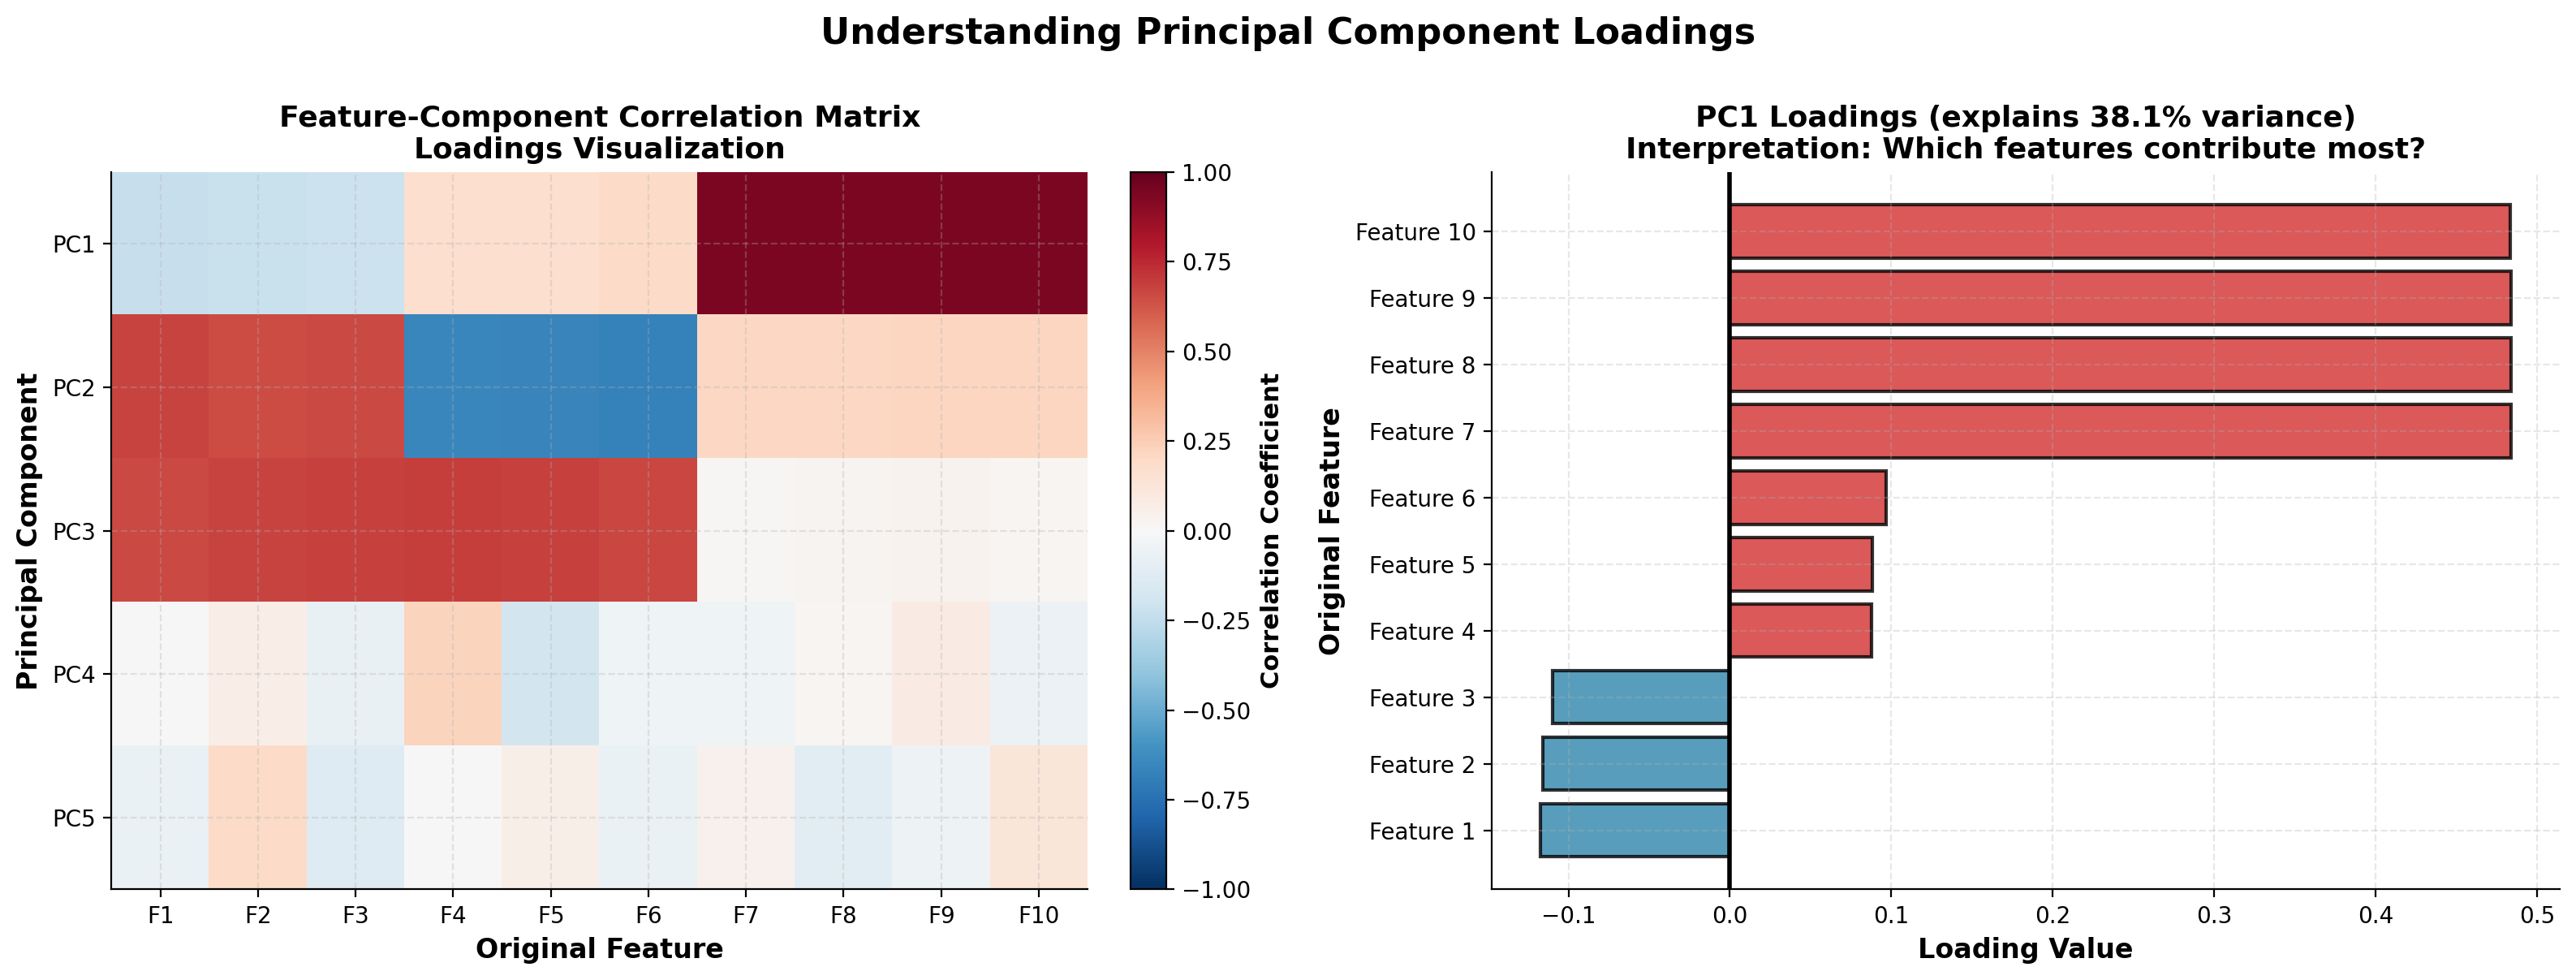
\includegraphics[width=\textwidth]{../figures/component_correlation.png}

\vspace{0.2cm}

\textbf{Example Loading Matrix:}

\begin{center}
\scriptsize
\begin{tabular}{|l|c|c|c|}
\hline
\textbf{Feature} & \textbf{PC1} & \textbf{PC2} & \textbf{PC3} \\
\hline
Height & 0.82 & 0.15 & -0.05 \\
Weight & 0.79 & 0.20 & 0.08 \\
Age & 0.12 & 0.91 & 0.10 \\
Income & -0.05 & 0.08 & 0.95 \\
\hline
\end{tabular}
\end{center}

\vspace{0.2cm}

\textbf{Interpretation:}
\begin{itemize}
\setlength{\itemsep}{2pt}
\item PC1: "Body size" (height, weight)
\item PC2: "Age" dimension
\item PC3: "Income" dimension
\item Clear separation of concepts
\end{itemize}
\end{column}
\end{columns}
\end{frame}

% ========================================
% Section: Applications
% ========================================

\section{Applications}

\begin{frame}{Application: Image Compression}
\begin{columns}[t]
\begin{column}{0.48\textwidth}
\textbf{Problem:}
Images contain redundant information. Can we store them more efficiently?

\vspace{0.2cm}

\textbf{PCA Approach:}
\begin{enumerate}
\setlength{\itemsep}{2pt}
\item Treat each image as vector (flatten pixels)
\item Build dataset: $\mathbf{X} \in \mathbb{R}^{n \times d}$
\item Apply PCA: Find eigenvectors
\item Project: $\mathbf{Z} = \mathbf{X}\mathbf{V}_k$
\item Store: $\mathbf{Z}$ and $\mathbf{V}_k$ instead of $\mathbf{X}$
\end{enumerate}

\vspace{0.2cm}

\textbf{Compression Ratio:}

Original: $n \times d$ values

Compressed: $n \times k + k \times d$ values

Ratio: $\frac{nd}{nk + kd} \approx \frac{d}{k}$ (for large $n$)

\vspace{0.2cm}

\textbf{Example:}
\begin{itemize}
\setlength{\itemsep}{0pt}
\item $d = 10,000$ pixels
\item $k = 100$ components
\item Compression: $100:1$
\end{itemize}
\end{column}

\begin{column}{0.48\textwidth}
\centering
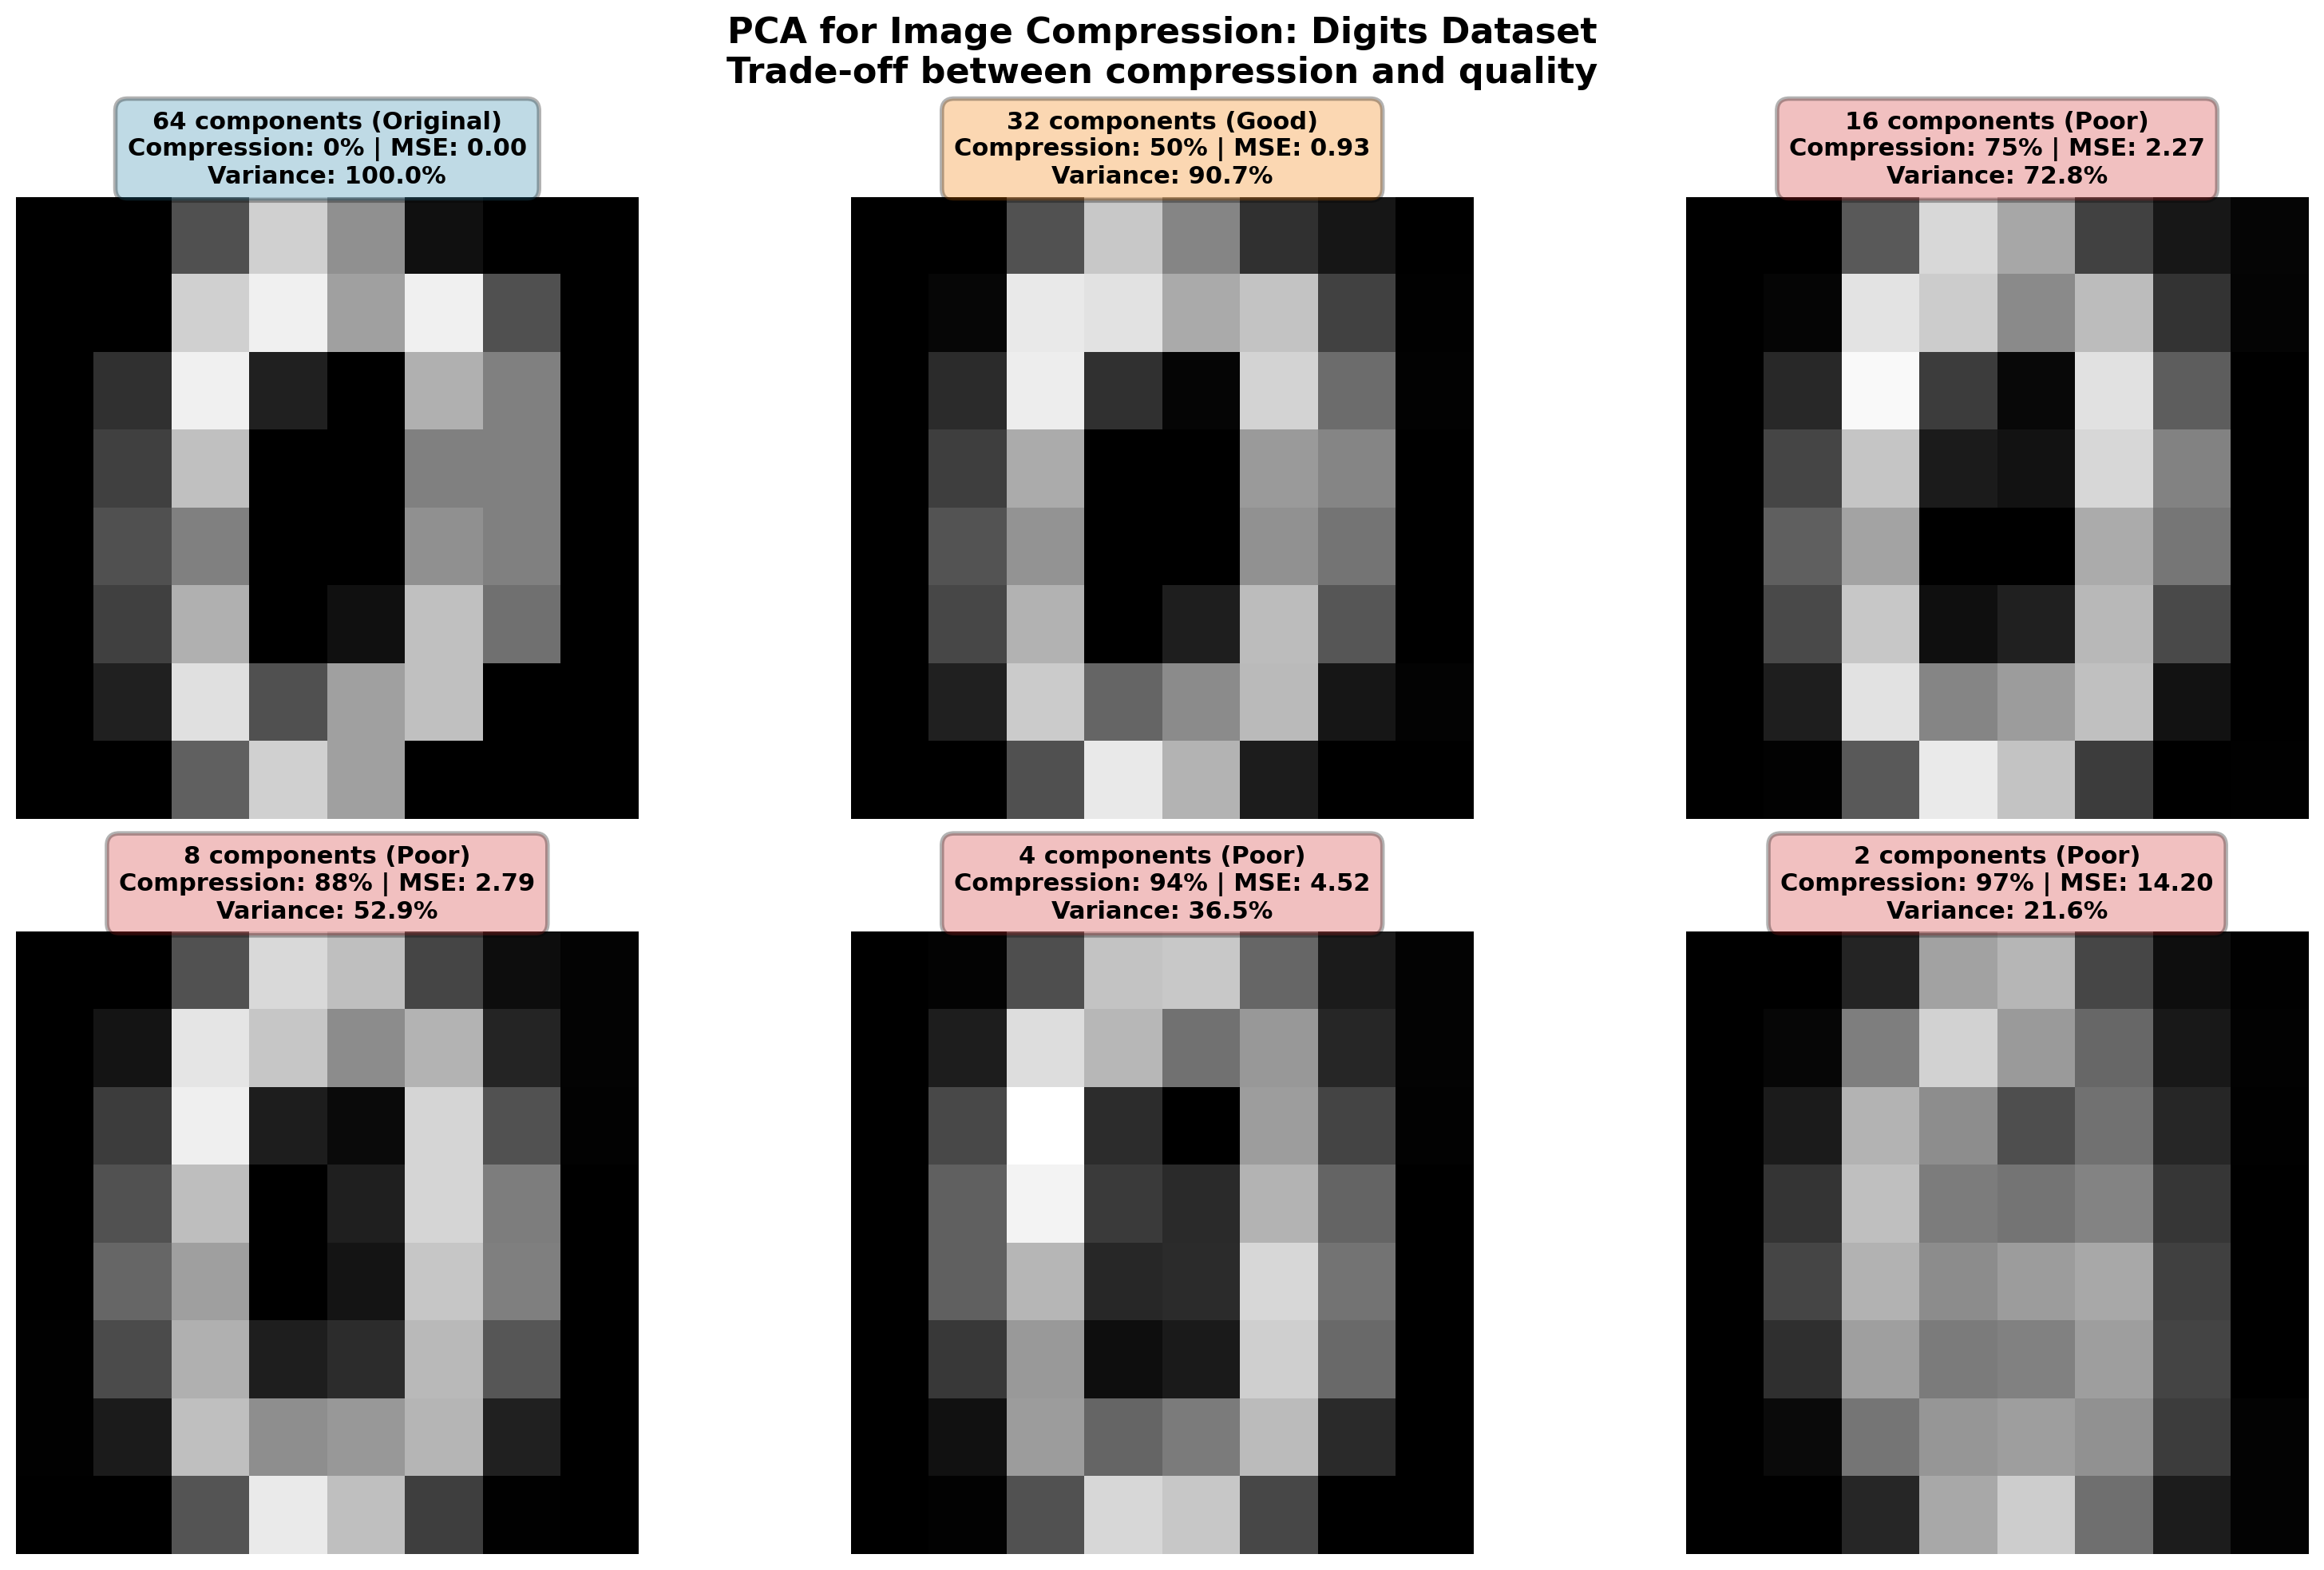
\includegraphics[width=\textwidth]{../figures/image_compression.png}

\vspace{0.2cm}

\textbf{Quality vs Compression:}

\begin{center}
\scriptsize
\begin{tabular}{|c|c|c|}
\hline
\textbf{PCs} & \textbf{Compression} & \textbf{Quality} \\
\hline
10 & 95\% & Poor \\
50 & 75\% & Fair \\
100 & 50\% & Good \\
200 & 0\% & Excellent \\
\hline
\end{tabular}
\end{center}

\vspace{0.2cm}

\begin{exampleblock}{Trade-off}
Balance between file size and visual quality. Typical choice: 80-90\% variance retained.
\end{exampleblock}
\end{column}
\end{columns}
\end{frame}

\begin{frame}{Application: Face Recognition (Eigenfaces)}
\begin{columns}[t]
\begin{column}{0.48\textwidth}
\textbf{Eigenfaces Method:}

\begin{enumerate}
\setlength{\itemsep}{2pt}
\item Collect face images: $n$ images, $d$ pixels each
\item Apply PCA: Find "eigenfaces" (principal components)
\item Each eigenface captures facial variation
\item Represent faces in eigenface space
\item Recognition: Nearest neighbor in PC space
\end{enumerate}

\vspace{0.2cm}

\textbf{Advantages:}
\begin{itemize}
\setlength{\itemsep}{2pt}
\item Dimensionality reduction: $10,000 \to 100$
\item Fast matching in low-dimensional space
\item Captures important facial features
\item Robust to minor variations
\end{itemize}

\vspace{0.2cm}

\textbf{Process:}
\begin{itemize}
\setlength{\itemsep}{2pt}
\item Training: Build eigenface basis
\item Enrollment: Project new face to PC space
\item Recognition: Compare with database
\item Decision: Threshold distance
\end{itemize}
\end{column}

\begin{column}{0.48\textwidth}
\centering
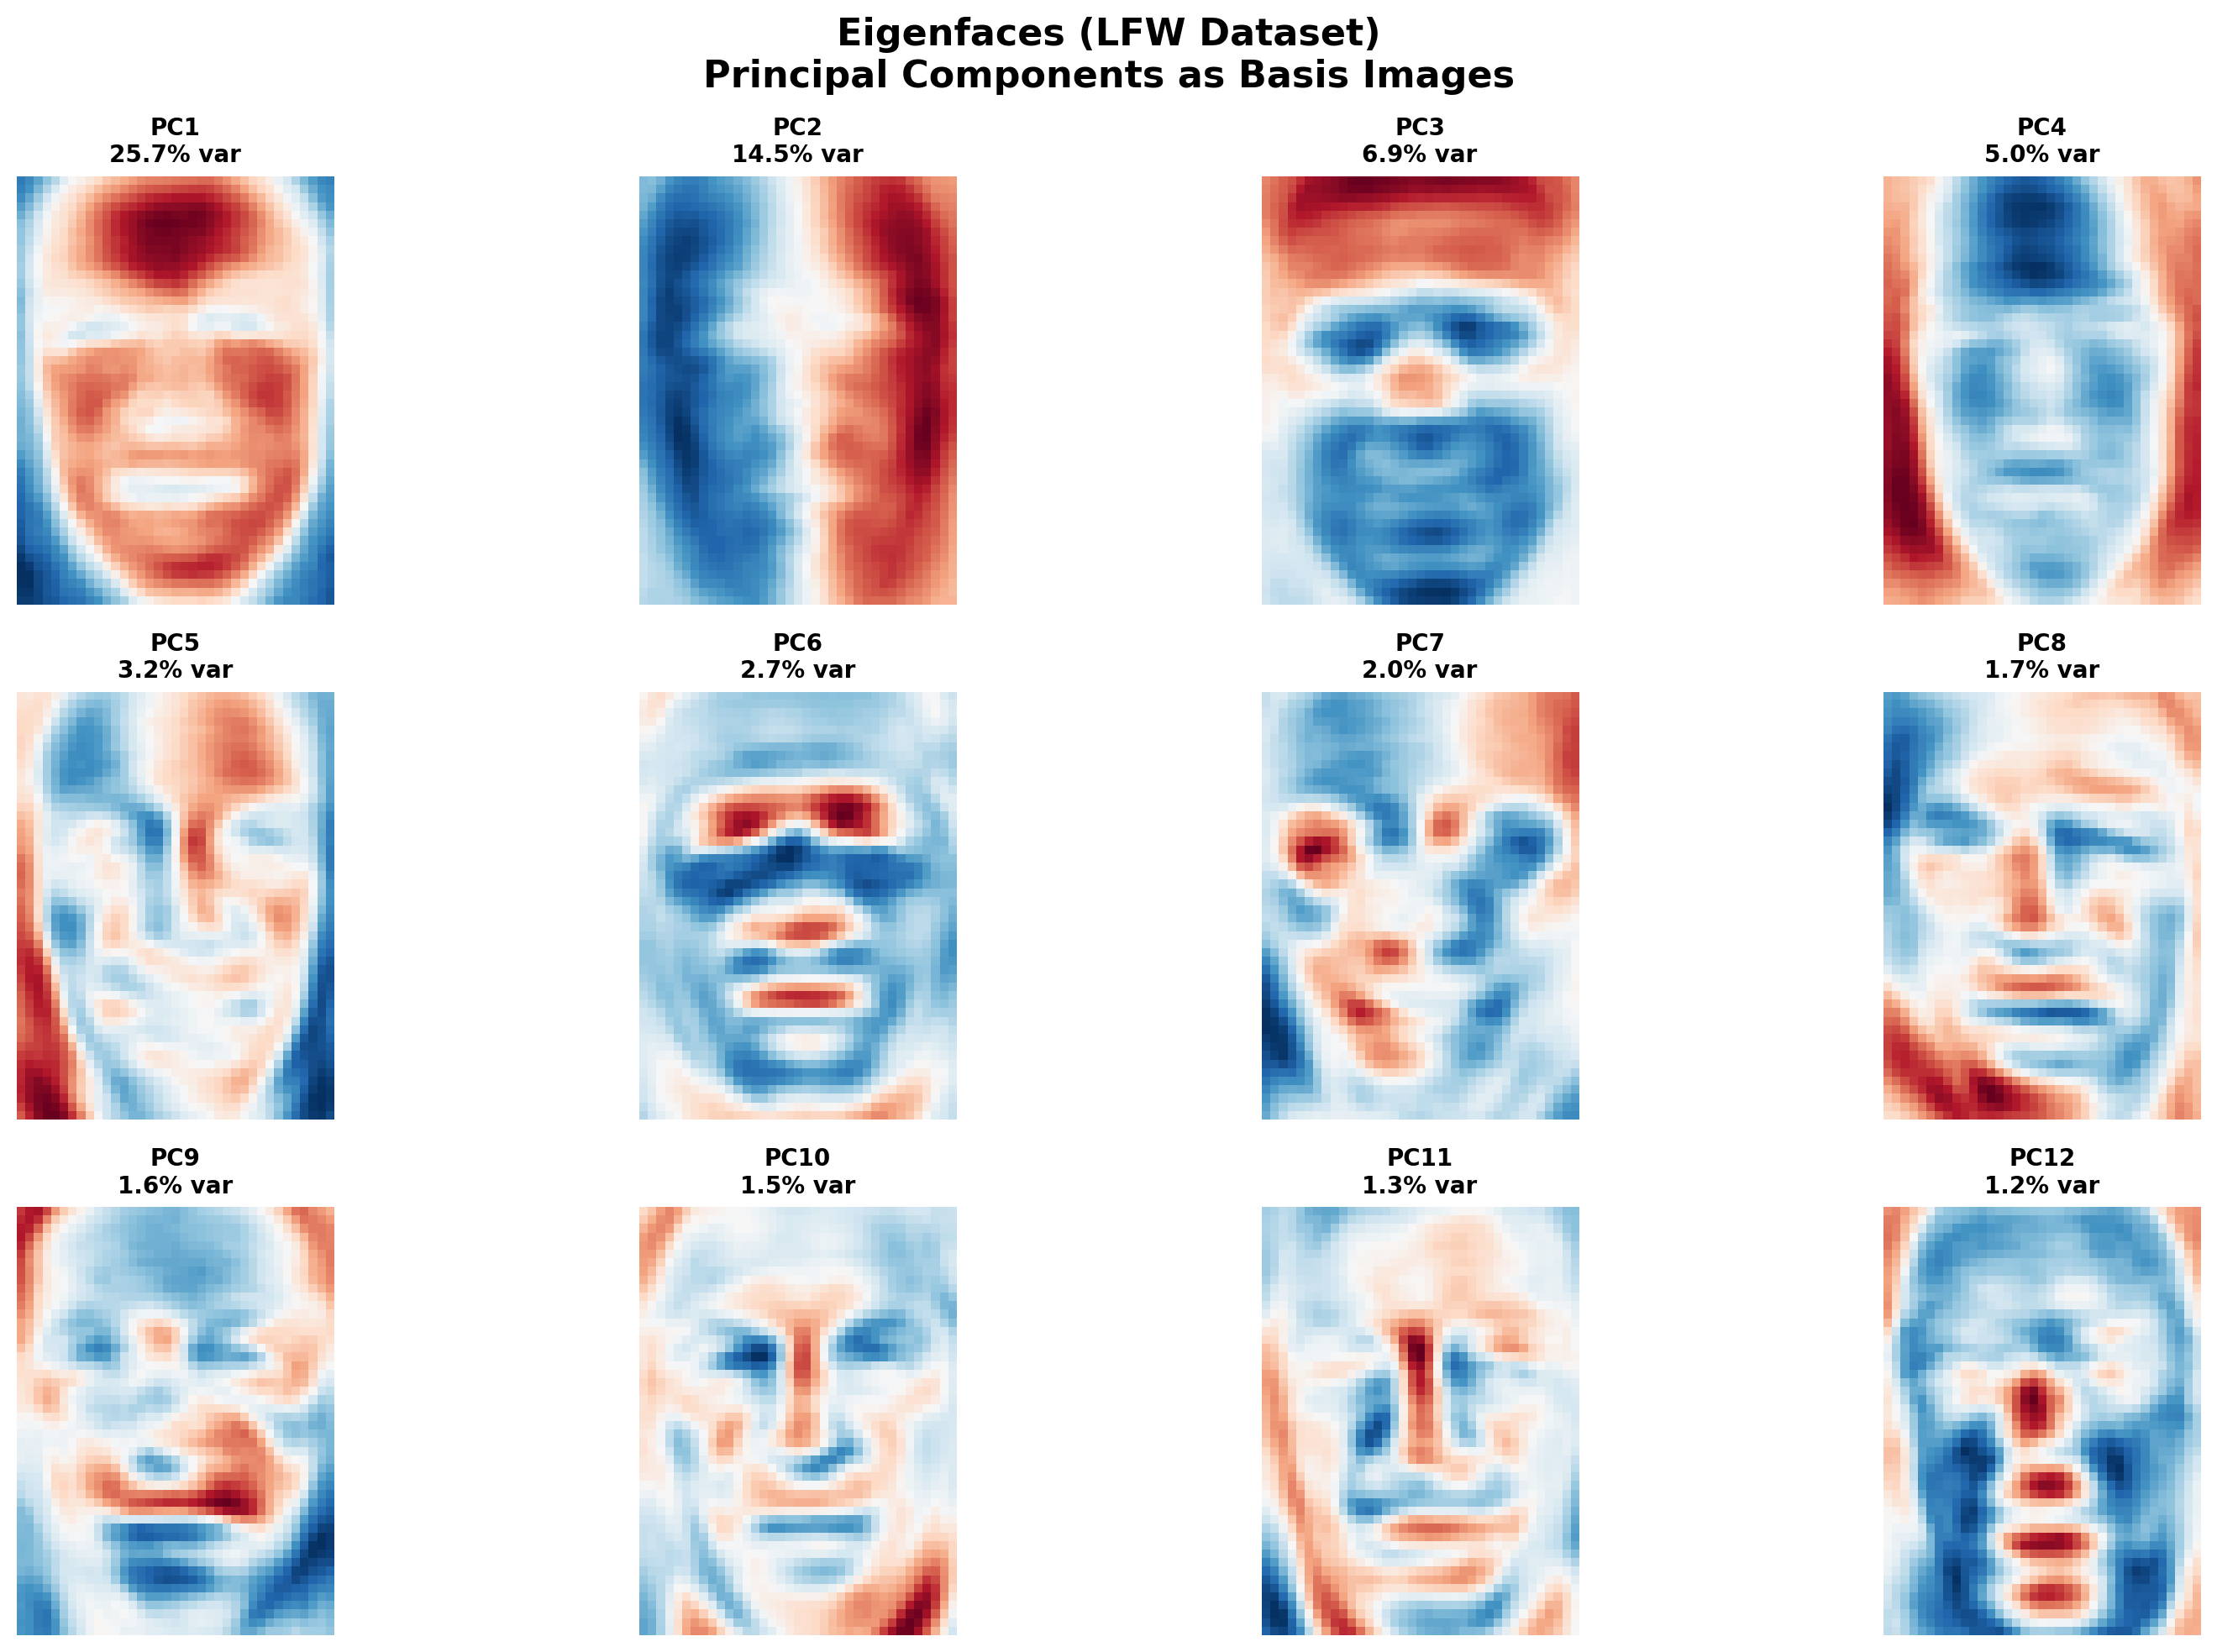
\includegraphics[width=\textwidth]{../figures/eigenfaces_application.png}

\vspace{0.2cm}

\textbf{Typical Eigenfaces:}
\begin{itemize}
\setlength{\itemsep}{2pt}
\item PC1: Average lighting
\item PC2: Left-right contrast
\item PC3: Facial expression
\item PC4-10: Detailed features
\item PC11+: Fine details/noise
\end{itemize}

\vspace{0.2cm}

\begin{exampleblock}{Historical Note}
Eigenfaces pioneered in 1991 by Turk and Pentland. Still used as baseline method.
\end{exampleblock}

\vspace{0.2cm}

\begin{alertblock}{Limitations}
Sensitive to: lighting, pose, facial expression. Modern methods use deep learning.
\end{alertblock}
\end{column}
\end{columns}
\end{frame}

\begin{frame}{Application: Noise Filtering}
\begin{columns}[t]
\begin{column}{0.48\textwidth}
\textbf{Principle:}

Noise typically has:
\begin{itemize}
\setlength{\itemsep}{2pt}
\item Low variance
\item High frequency
\item Random direction
\item Captured by small eigenvalues
\end{itemize}

Signal has:
\begin{itemize}
\setlength{\itemsep}{2pt}
\item High variance
\item Low frequency
\item Structured patterns
\item Captured by large eigenvalues
\end{itemize}

\vspace{0.2cm}

\textbf{Denoising Procedure:}
\begin{enumerate}
\setlength{\itemsep}{2pt}
\item Apply PCA to noisy data
\item Keep only top $k$ components (signal)
\item Discard remaining components (noise)
\item Reconstruct: $\hat{\mathbf{X}} = \mathbf{X}\mathbf{V}_k\mathbf{V}_k^T$
\end{enumerate}

\vspace{0.2cm}

\begin{alertblock}{Key Insight}
PCA acts as low-pass filter, removing high-frequency noise.
\end{alertblock}
\end{column}

\begin{column}{0.48\textwidth}
\centering
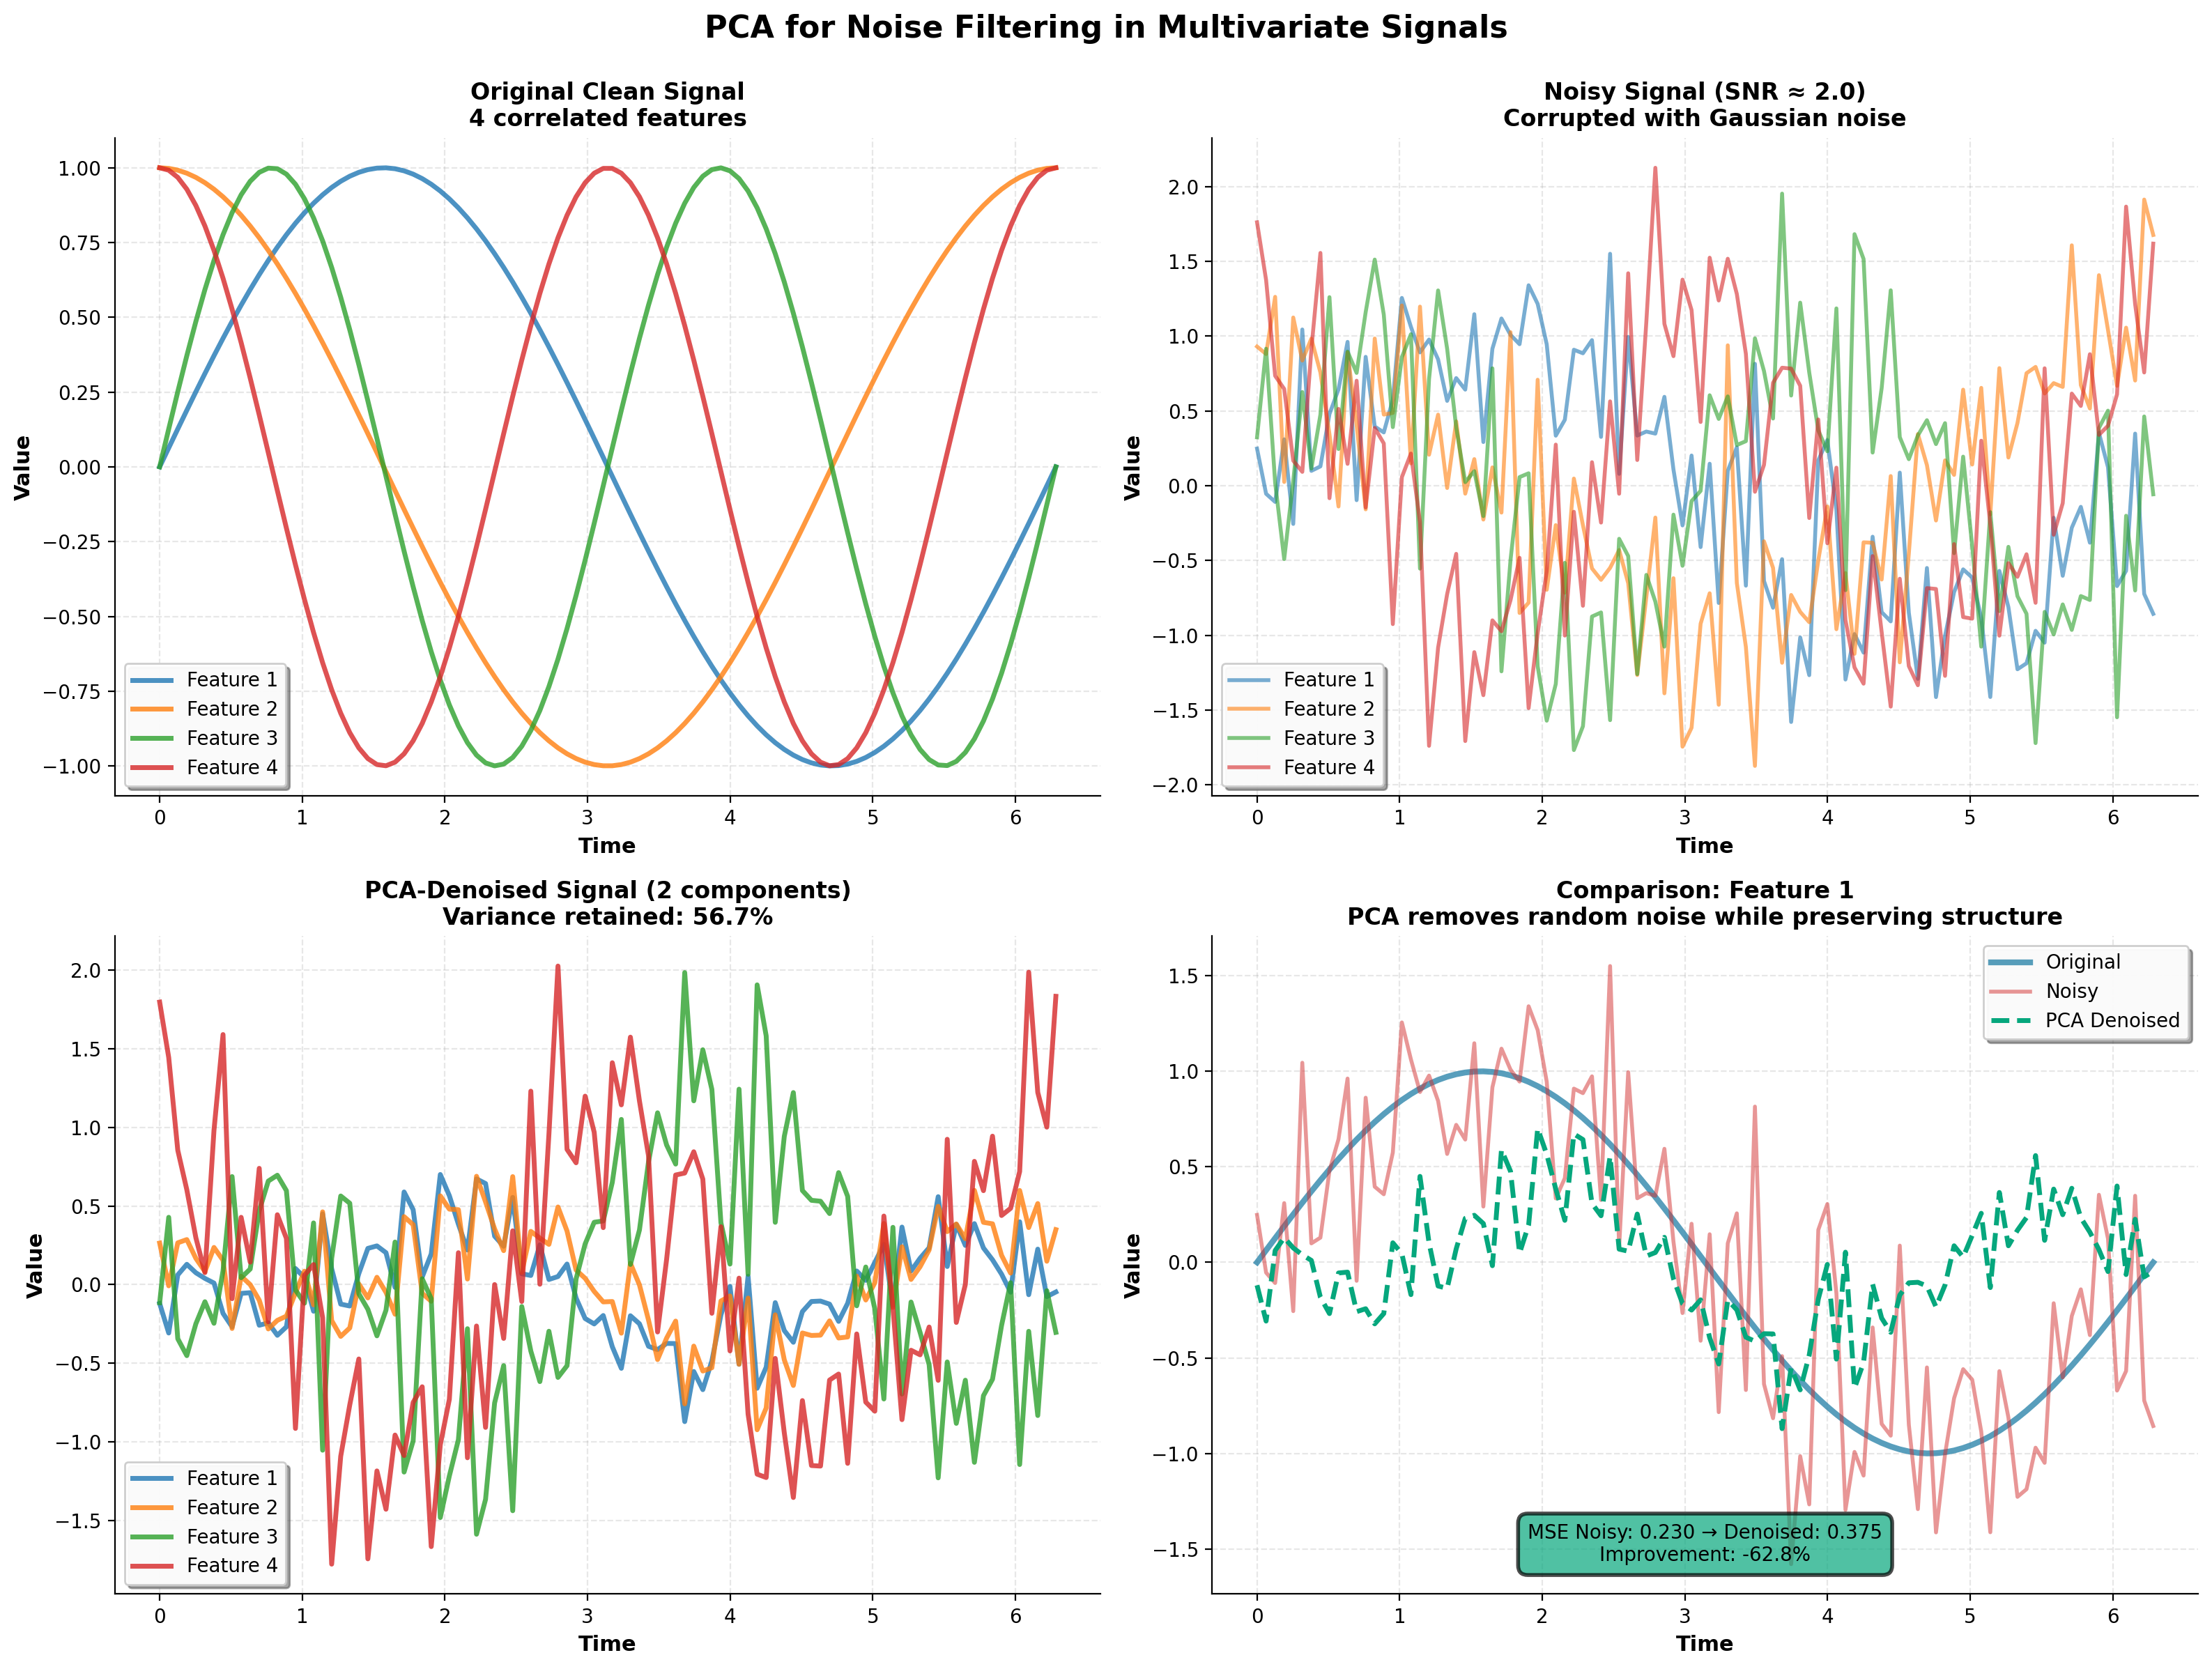
\includegraphics[width=\textwidth]{../figures/noise_filtering.png}

\vspace{0.2cm}

\textbf{Example: Signal Denoising}

Original signal + Gaussian noise

\begin{itemize}
\setlength{\itemsep}{2pt}
\item Noise variance: 0.1
\item PCA: Keep 5 components
\item SNR improvement: 15 dB
\end{itemize}

\vspace{0.2cm}

\textbf{Applications:}
\begin{itemize}
\setlength{\itemsep}{2pt}
\item Image denoising
\item Audio signal processing
\item Sensor data cleaning
\item Medical imaging
\item Financial time series
\end{itemize}

\vspace{0.2cm}

\begin{exampleblock}{Challenge}
Choosing $k$: Too small loses signal, too large keeps noise. Use cross-validation or domain knowledge.
\end{exampleblock}
\end{column}
\end{columns}
\end{frame}

\begin{frame}{Application: Data Visualization}
\begin{columns}[t]
\begin{column}{0.48\textwidth}
\textbf{Challenge:}

Cannot visualize data in $d > 3$ dimensions.

\vspace{0.2cm}

\textbf{PCA Solution:}

Project to 2D or 3D for visualization:
\begin{enumerate}
\setlength{\itemsep}{2pt}
\item Apply PCA: Get principal components
\item Keep PC1 and PC2 (or PC1, PC2, PC3)
\item Plot data in reduced space
\item Preserves maximum variance
\end{enumerate}

\vspace{0.2cm}

\textbf{Interpretation:}
\begin{itemize}
\setlength{\itemsep}{2pt}
\item PC1 (x-axis): Direction of most variance
\item PC2 (y-axis): Second most variance
\item Distances approximately preserved
\item Clusters may emerge
\end{itemize}

\vspace{0.2cm}

\textbf{Use Cases:}
\begin{itemize}
\setlength{\itemsep}{2pt}
\item Exploratory data analysis
\item Cluster visualization
\item Outlier detection
\item Pattern discovery
\item Presentation to stakeholders
\end{itemize}
\end{column}

\begin{column}{0.48\textwidth}
\centering
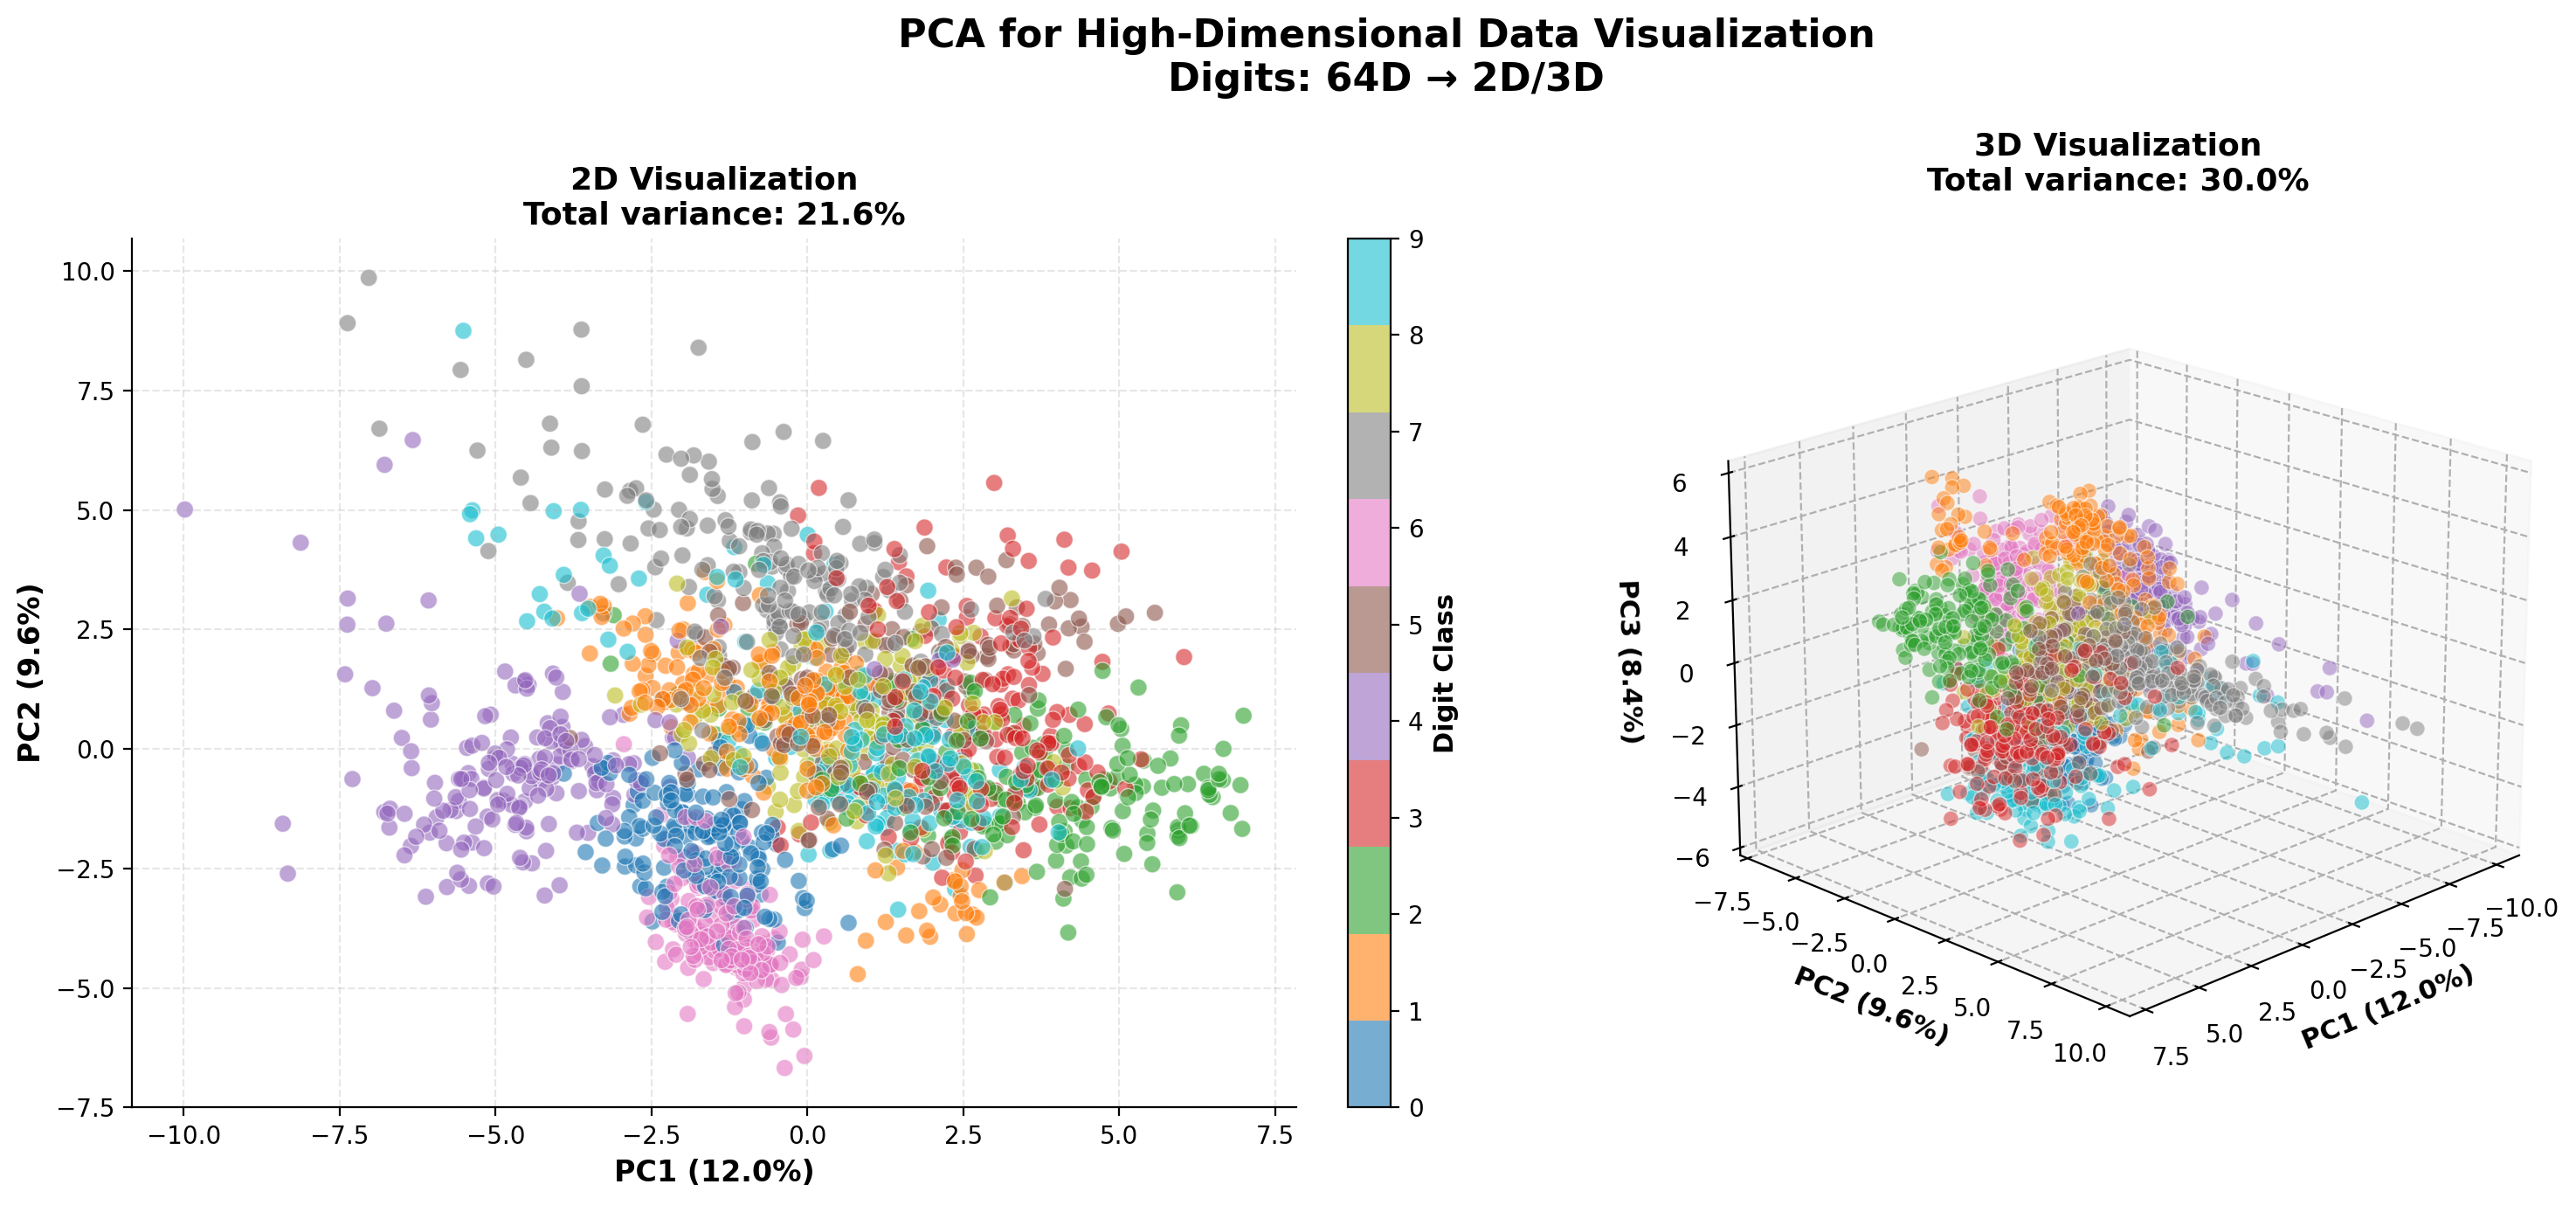
\includegraphics[width=\textwidth]{../figures/data_visualization_application.png}

\vspace{0.2cm}

\begin{exampleblock}{Example: Iris Dataset}
\begin{itemize}
\setlength{\itemsep}{2pt}
\item Original: 4 dimensions
\item PCA: 2D projection
\item Explained variance: 95.8\%
\item Clear species separation visible
\end{itemize}
\end{exampleblock}

\vspace{0.2cm}

\textbf{Comparison with Other Methods:}

\begin{center}
\scriptsize
\begin{tabular}{|l|c|c|}
\hline
\textbf{Method} & \textbf{Linear} & \textbf{Global} \\
\hline
PCA & Yes & Yes \\
t-SNE & No & No \\
UMAP & No & Local \\
MDS & Yes/No & Yes \\
\hline
\end{tabular}
\end{center}

\vspace{0.2cm}

\begin{alertblock}{Limitation}
PCA preserves global structure but may miss non-linear patterns.
\end{alertblock}
\end{column}
\end{columns}
\end{frame}

\begin{frame}{Application: Exploratory Data Analysis}
\begin{columns}[t]
\begin{column}{0.48\textwidth}
\textbf{Digits Dataset Visualization:}

High-dimensional handwritten digit images (64 dimensions) projected to 2D.

\vspace{0.2cm}

\textbf{Insights from PCA:}
\begin{itemize}
\setlength{\itemsep}{2pt}
\item Digit clusters visible in PC space
\item Similar digits closer together
\item Outliers easily identified
\item Confusion patterns apparent
\end{itemize}

\vspace{0.2cm}

\textbf{Practical Workflow:}
\begin{enumerate}
\setlength{\itemsep}{2pt}
\item Load dataset
\item Standardize features
\item Apply PCA (keep 2-3 PCs)
\item Visualize with scatter plot
\item Color by labels (if available)
\item Identify patterns/outliers
\end{enumerate}

\vspace{0.2cm}

\begin{alertblock}{EDA Benefit}
Quick visual check before applying complex ML models.
\end{alertblock}
\end{column}

\begin{column}{0.48\textwidth}
\centering
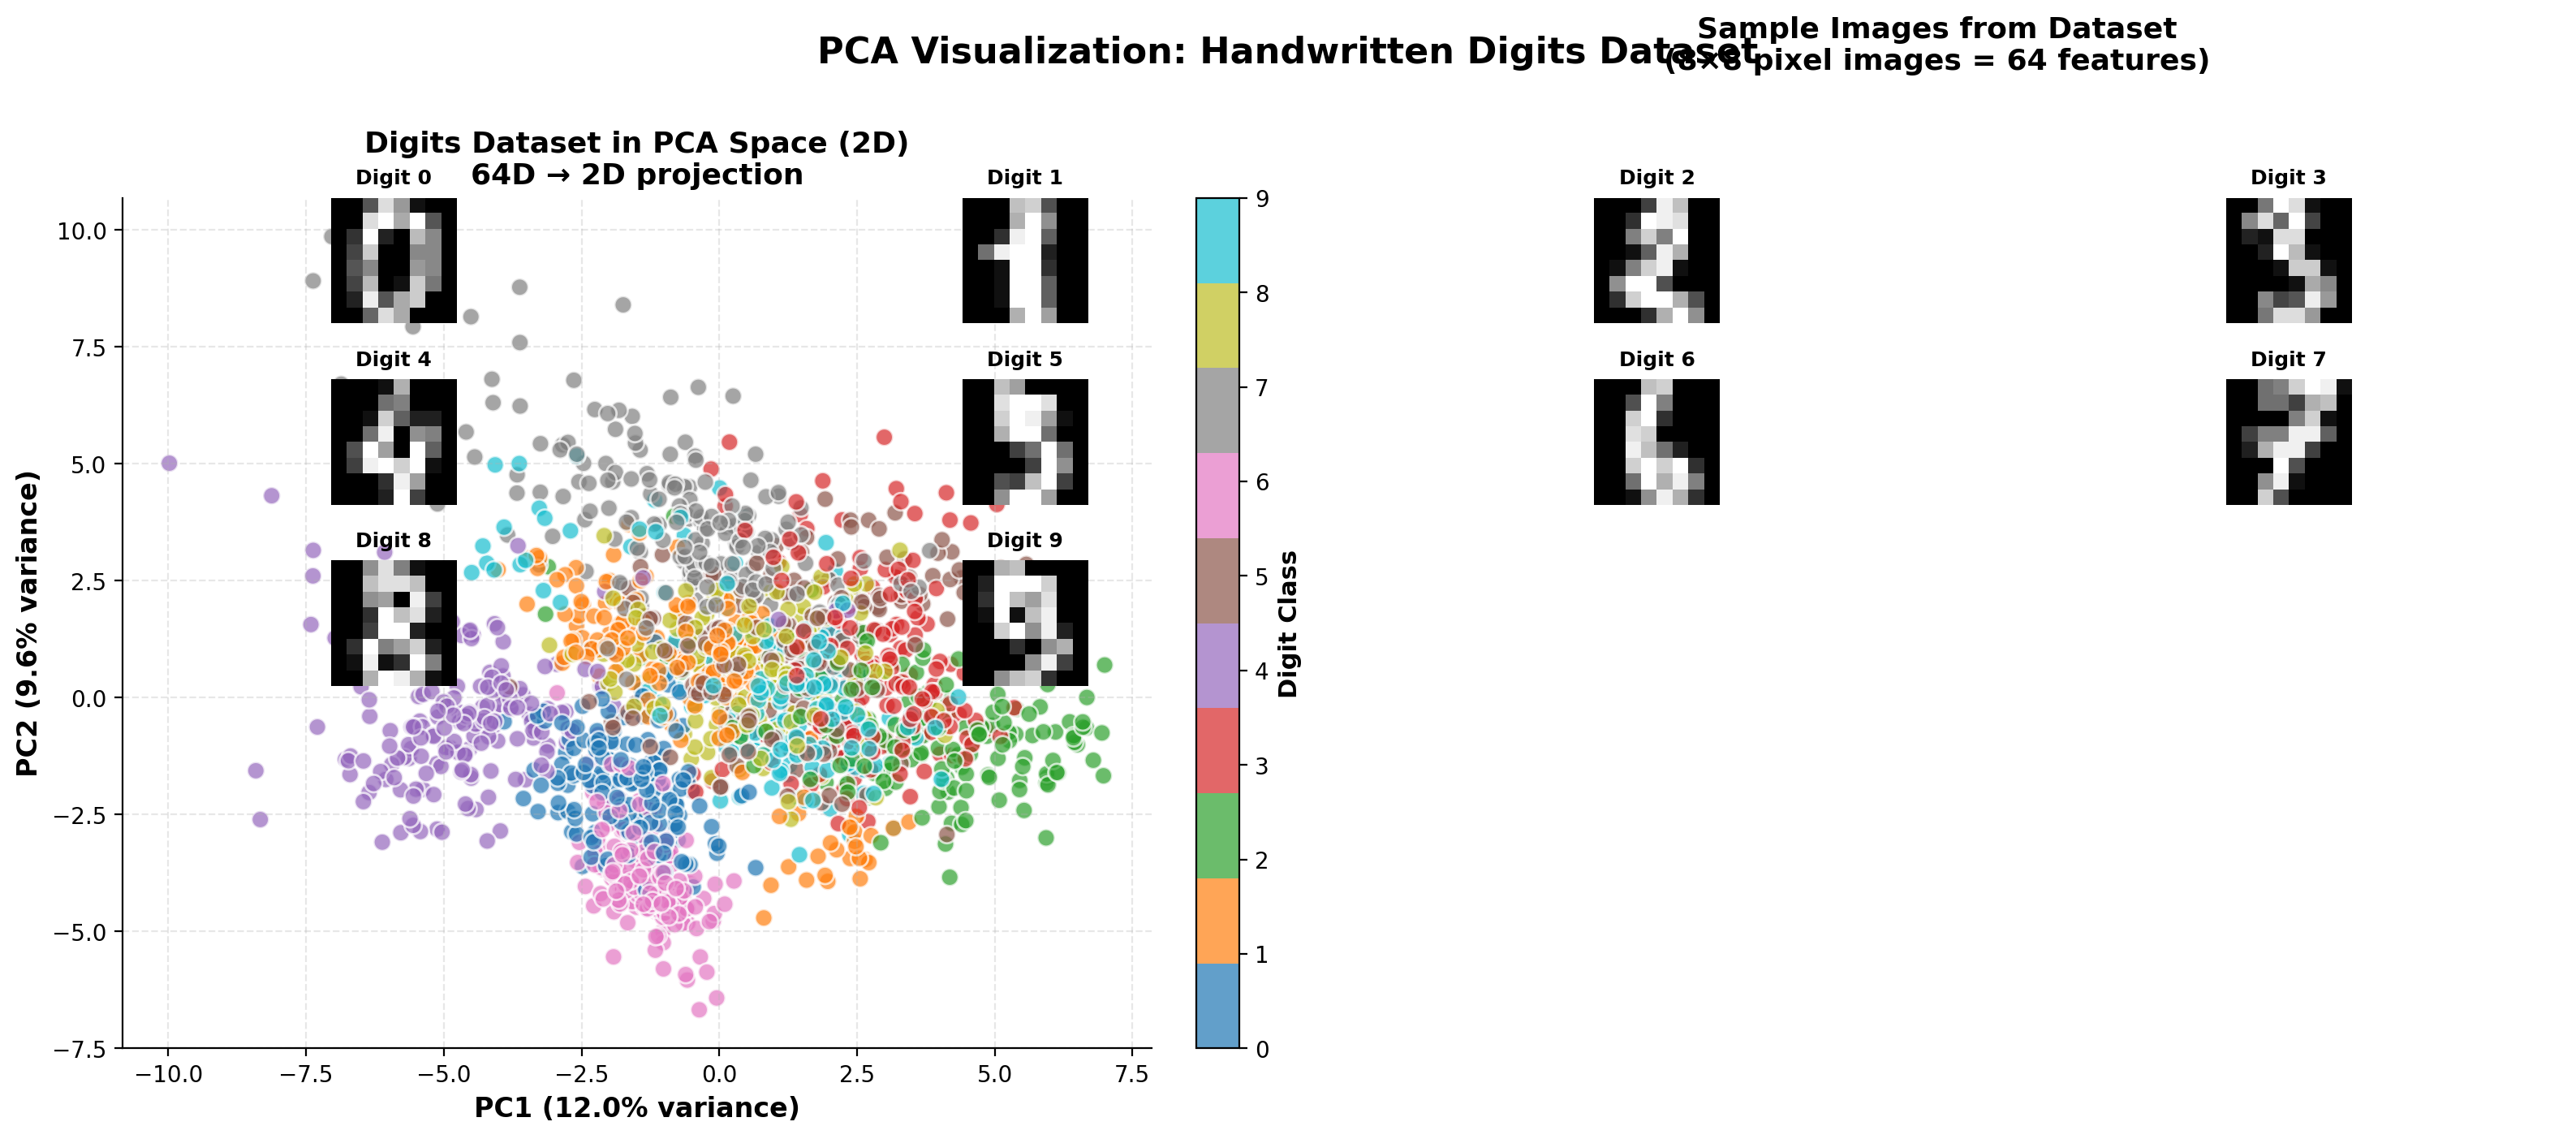
\includegraphics[width=\textwidth]{../figures/digits_visualization.png}

\vspace{0.2cm}

\textbf{Observations:}
\begin{itemize}
\setlength{\itemsep}{2pt}
\item Digits 0 and 1 well-separated
\item Digits 3, 5, 8 overlap slightly
\item Some outliers (miswritten digits)
\item PC1 and PC2 capture 30\% variance
\end{itemize}

\vspace{0.2cm}

\begin{exampleblock}{Feature Engineering}
PCA projections can be used as features for downstream classification:
\begin{itemize}
\setlength{\itemsep}{0pt}
\item Reduce 64D to 20D
\item Train classifier on PC scores
\item Faster training
\item Often better generalization
\end{itemize}
\end{exampleblock}
\end{column}
\end{columns}
\end{frame}

\begin{frame}{Application: Feature Engineering}
\begin{columns}[t]
\begin{column}{0.48\textwidth}
\textbf{PCA as Preprocessing:}

Use PCA-transformed features for ML models.

\vspace{0.2cm}

\textbf{Benefits:}
\begin{itemize}
\setlength{\itemsep}{2pt}
\item \textbf{Decorrelation:} Remove multicollinearity
\item \textbf{Dimensionality:} Reduce feature count
\item \textbf{Noise reduction:} Filter out noisy components
\item \textbf{Speed:} Faster model training
\item \textbf{Regularization:} Implicit regularization effect
\end{itemize}

\vspace{0.2cm}

\textbf{Pipeline:}
\begin{algorithmic}[1]
\STATE Train set: Fit PCA
\STATE Train set: Transform with PCA
\STATE Test set: Transform with same PCA
\STATE Train classifier on PC scores
\STATE Evaluate on test PC scores
\end{algorithmic}

\vspace{0.2cm}

\begin{alertblock}{Warning}
Never fit PCA on test data! This causes data leakage.
\end{alertblock}
\end{column}

\begin{column}{0.48\textwidth}
\centering
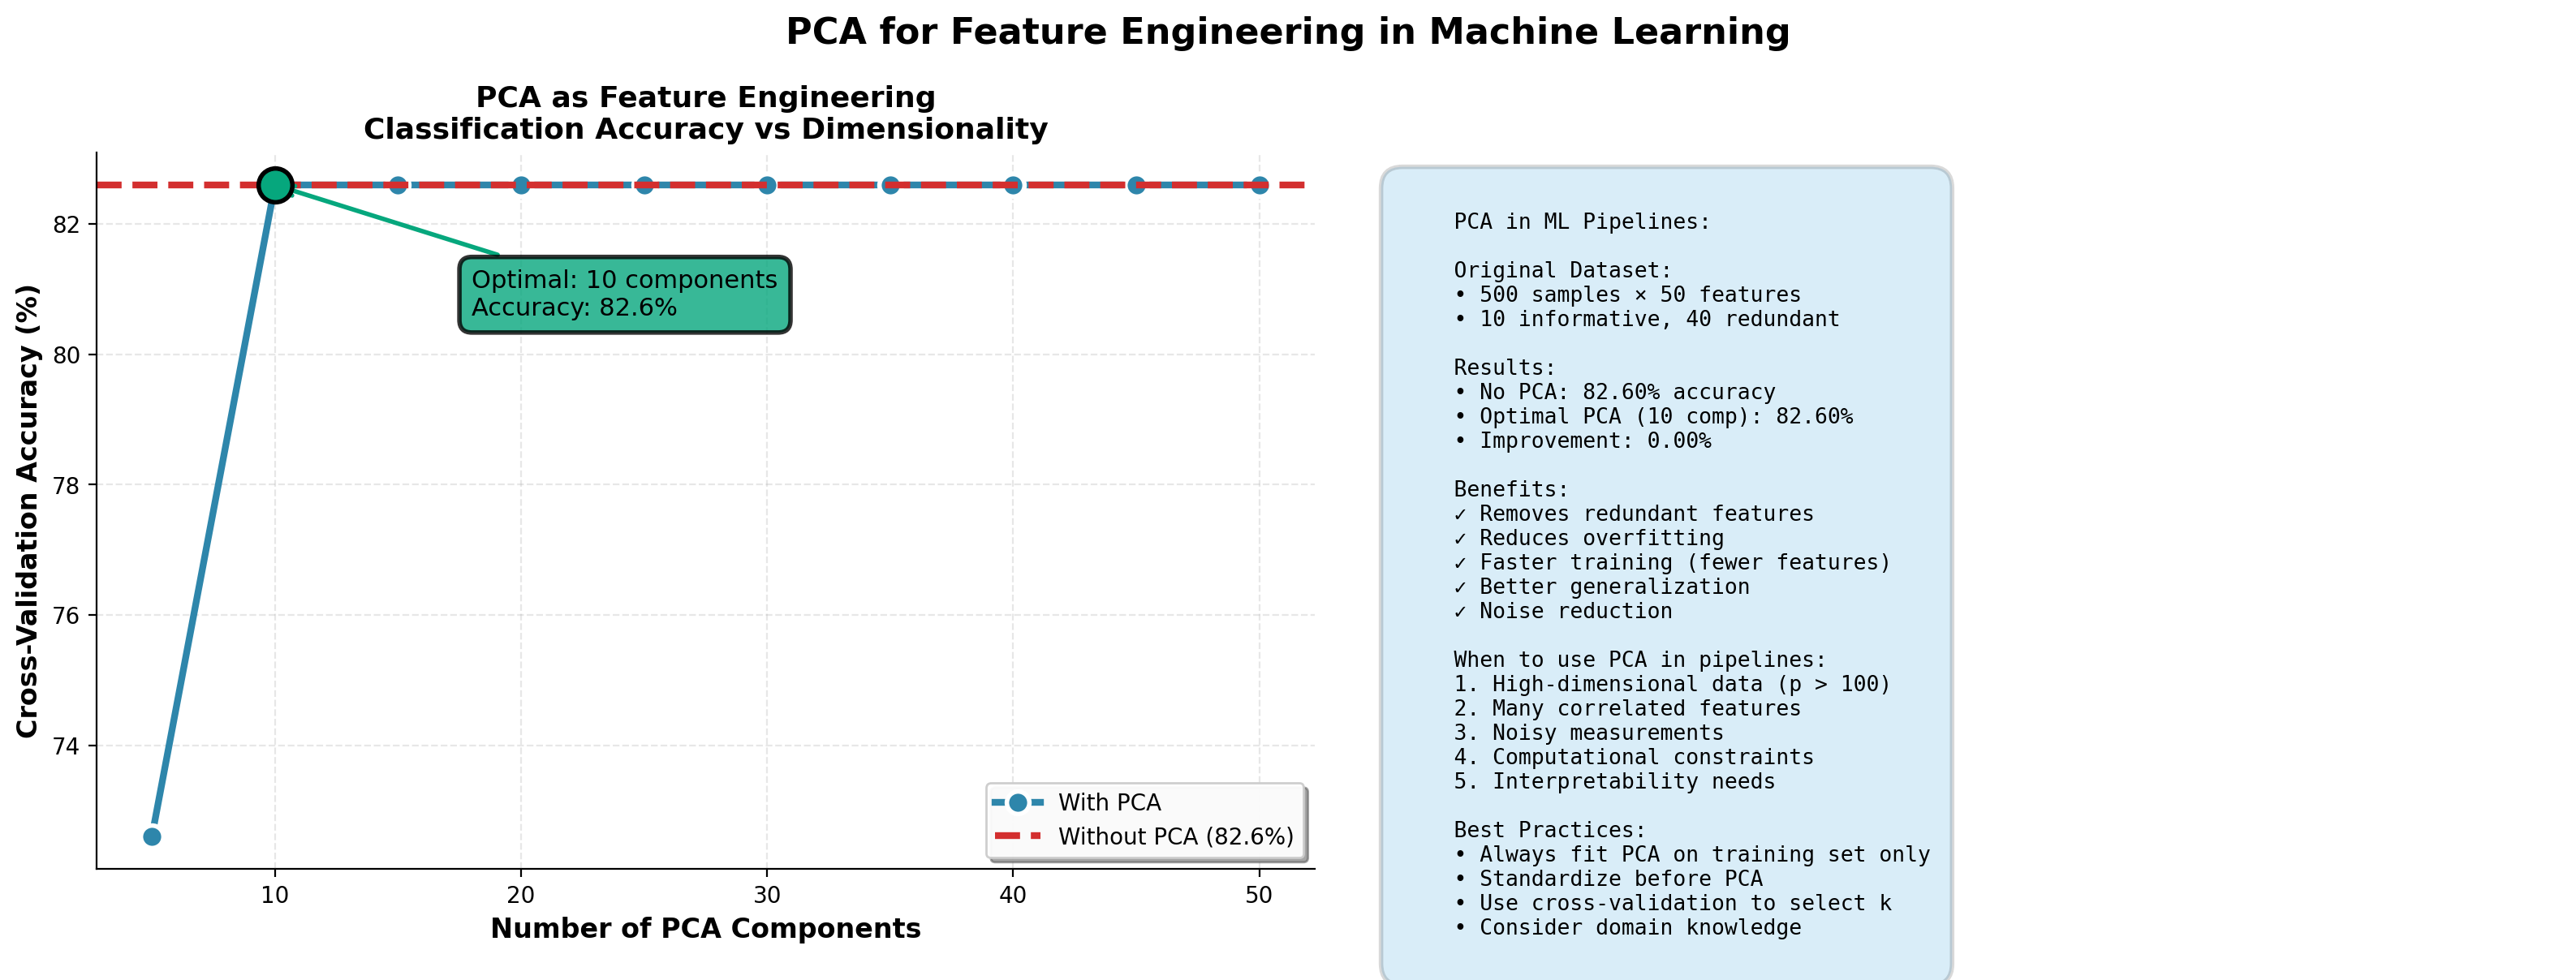
\includegraphics[width=\textwidth]{../figures/feature_engineering_application.png}

\vspace{0.2cm}

\textbf{Example Results:}

\begin{center}
\scriptsize
\begin{tabular}{|l|c|c|}
\hline
\textbf{Features} & \textbf{Accuracy} & \textbf{Time} \\
\hline
Original (1000D) & 0.85 & 120s \\
PCA (100D) & 0.87 & 15s \\
PCA (50D) & 0.86 & 8s \\
PCA (10D) & 0.79 & 2s \\
\hline
\end{tabular}
\end{center}

\vspace{0.2cm}

\textbf{Observations:}
\begin{itemize}
\setlength{\itemsep}{2pt}
\item Sweet spot: 50-100 components
\item Improved accuracy with PCA
\item Much faster training
\item Slight degradation with too few PCs
\end{itemize}

\vspace{0.2cm}

\begin{exampleblock}{Use Case}
High-dimensional datasets where features are correlated (genomics, text, images).
\end{exampleblock}
\end{column}
\end{columns}
\end{frame}

% ========================================
% Section: Best Practices
% ========================================

\section{Best Practices \& Pitfalls}

\begin{frame}{Best Practices: Standardization}
\begin{columns}[t]
\begin{column}{0.48\textwidth}
\begin{alertblock}{Critical Decision}
Should you standardize features before PCA?
\end{alertblock}

\vspace{0.2cm}

\textbf{Standardization:}
$$z_j = \frac{x_j - \mu_j}{\sigma_j}$$

\vspace{0.2cm}

\textbf{When to Standardize:}
\begin{itemize}
\setlength{\itemsep}{2pt}
\item Features have different units
\item Features have different scales
\item Want equal weight for all features
\item Domain knowledge suggests equal importance
\end{itemize}

\vspace{0.2cm}

\textbf{When NOT to Standardize:}
\begin{itemize}
\setlength{\itemsep}{2pt}
\item Features already on same scale
\item Scale carries information
\item Domain knowledge: some features more important
\item Interpretation requires original scale
\end{itemize}
\end{column}

\begin{column}{0.48\textwidth}
\centering
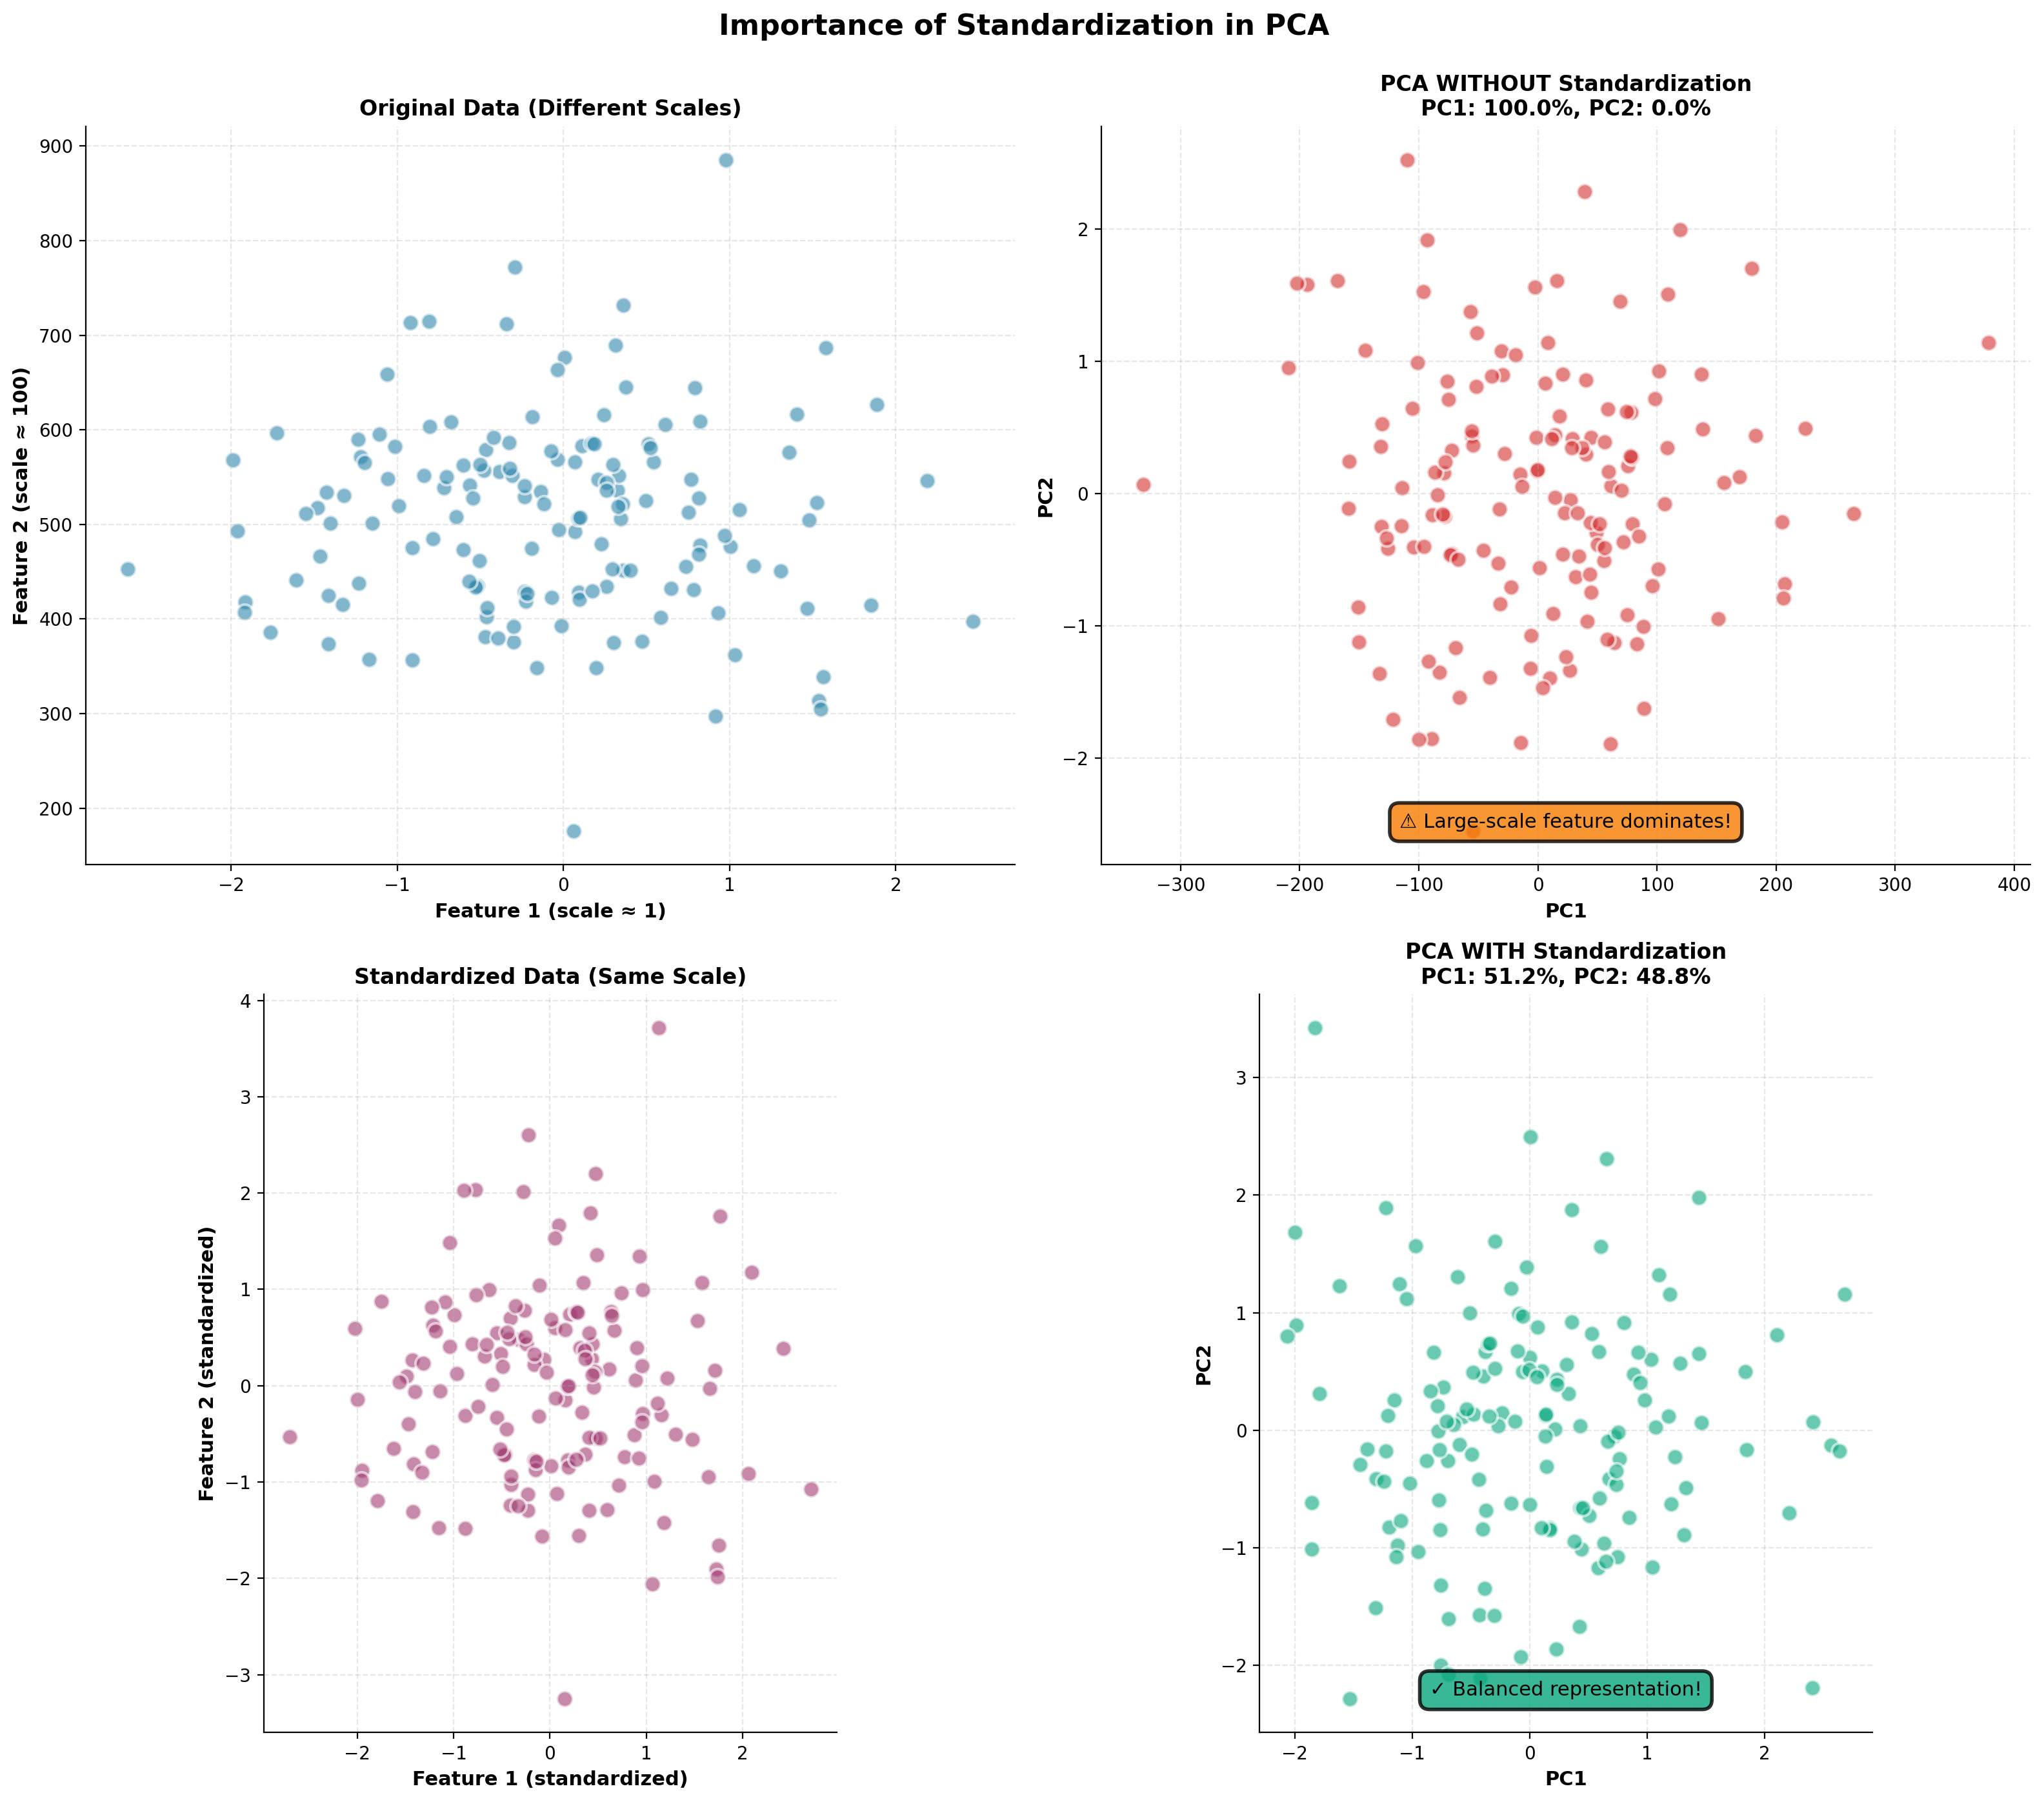
\includegraphics[width=\textwidth]{../figures/standardization_importance.png}

\vspace{0.2cm}

\textbf{Example Impact:}

Dataset: Height (cm), Weight (kg), Age (years)

\vspace{0.1cm}

\textit{Without standardization:}
\begin{itemize}
\setlength{\itemsep}{0pt}
\item Height range: 150-200
\item Weight range: 50-100
\item Age range: 20-70
\item PC1 dominated by height
\end{itemize}

\vspace{0.1cm}

\textit{With standardization:}
\begin{itemize}
\setlength{\itemsep}{0pt}
\item All ranges: -2 to 2
\item Equal opportunity for all
\item More balanced PCs
\end{itemize}

\vspace{0.2cm}

\begin{exampleblock}{Recommendation}
\textbf{Default: Standardize unless you have good reason not to.}
\end{exampleblock}
\end{column}
\end{columns}
\end{frame}

\begin{frame}{Computational Complexity}
\begin{columns}[t]
\begin{column}{0.48\textwidth}
\textbf{Standard PCA Complexity:}

\vspace{0.2cm}

\begin{tabular}{|l|c|}
\hline
\textbf{Operation} & \textbf{Complexity} \\
\hline
Centering & $\mathcal{O}(nd)$ \\
Covariance & $\mathcal{O}(nd^2)$ \\
Eigendecomp & $\mathcal{O}(d^3)$ \\
SVD & $\mathcal{O}(\min(nd^2, n^2d))$ \\
\hline
\textbf{Total} & $\mathcal{O}(nd^2 + d^3)$ \\
\hline
\end{tabular}

\vspace{0.2cm}

\textbf{Memory Requirements:}
\begin{itemize}
\setlength{\itemsep}{2pt}
\item Data: $\mathcal{O}(nd)$
\item Covariance: $\mathcal{O}(d^2)$
\item Eigenvectors: $\mathcal{O}(d^2)$
\item \textbf{Total:} $\mathcal{O}(nd + d^2)$
\end{itemize}

\vspace{0.2cm}

\textbf{Scalability Issues:}
\begin{itemize}
\setlength{\itemsep}{2pt}
\item Large $d$: Covariance matrix huge
\item Large $n$: Memory for data matrix
\item Both large: Computational bottleneck
\end{itemize}
\end{column}

\begin{column}{0.48\textwidth}
\centering
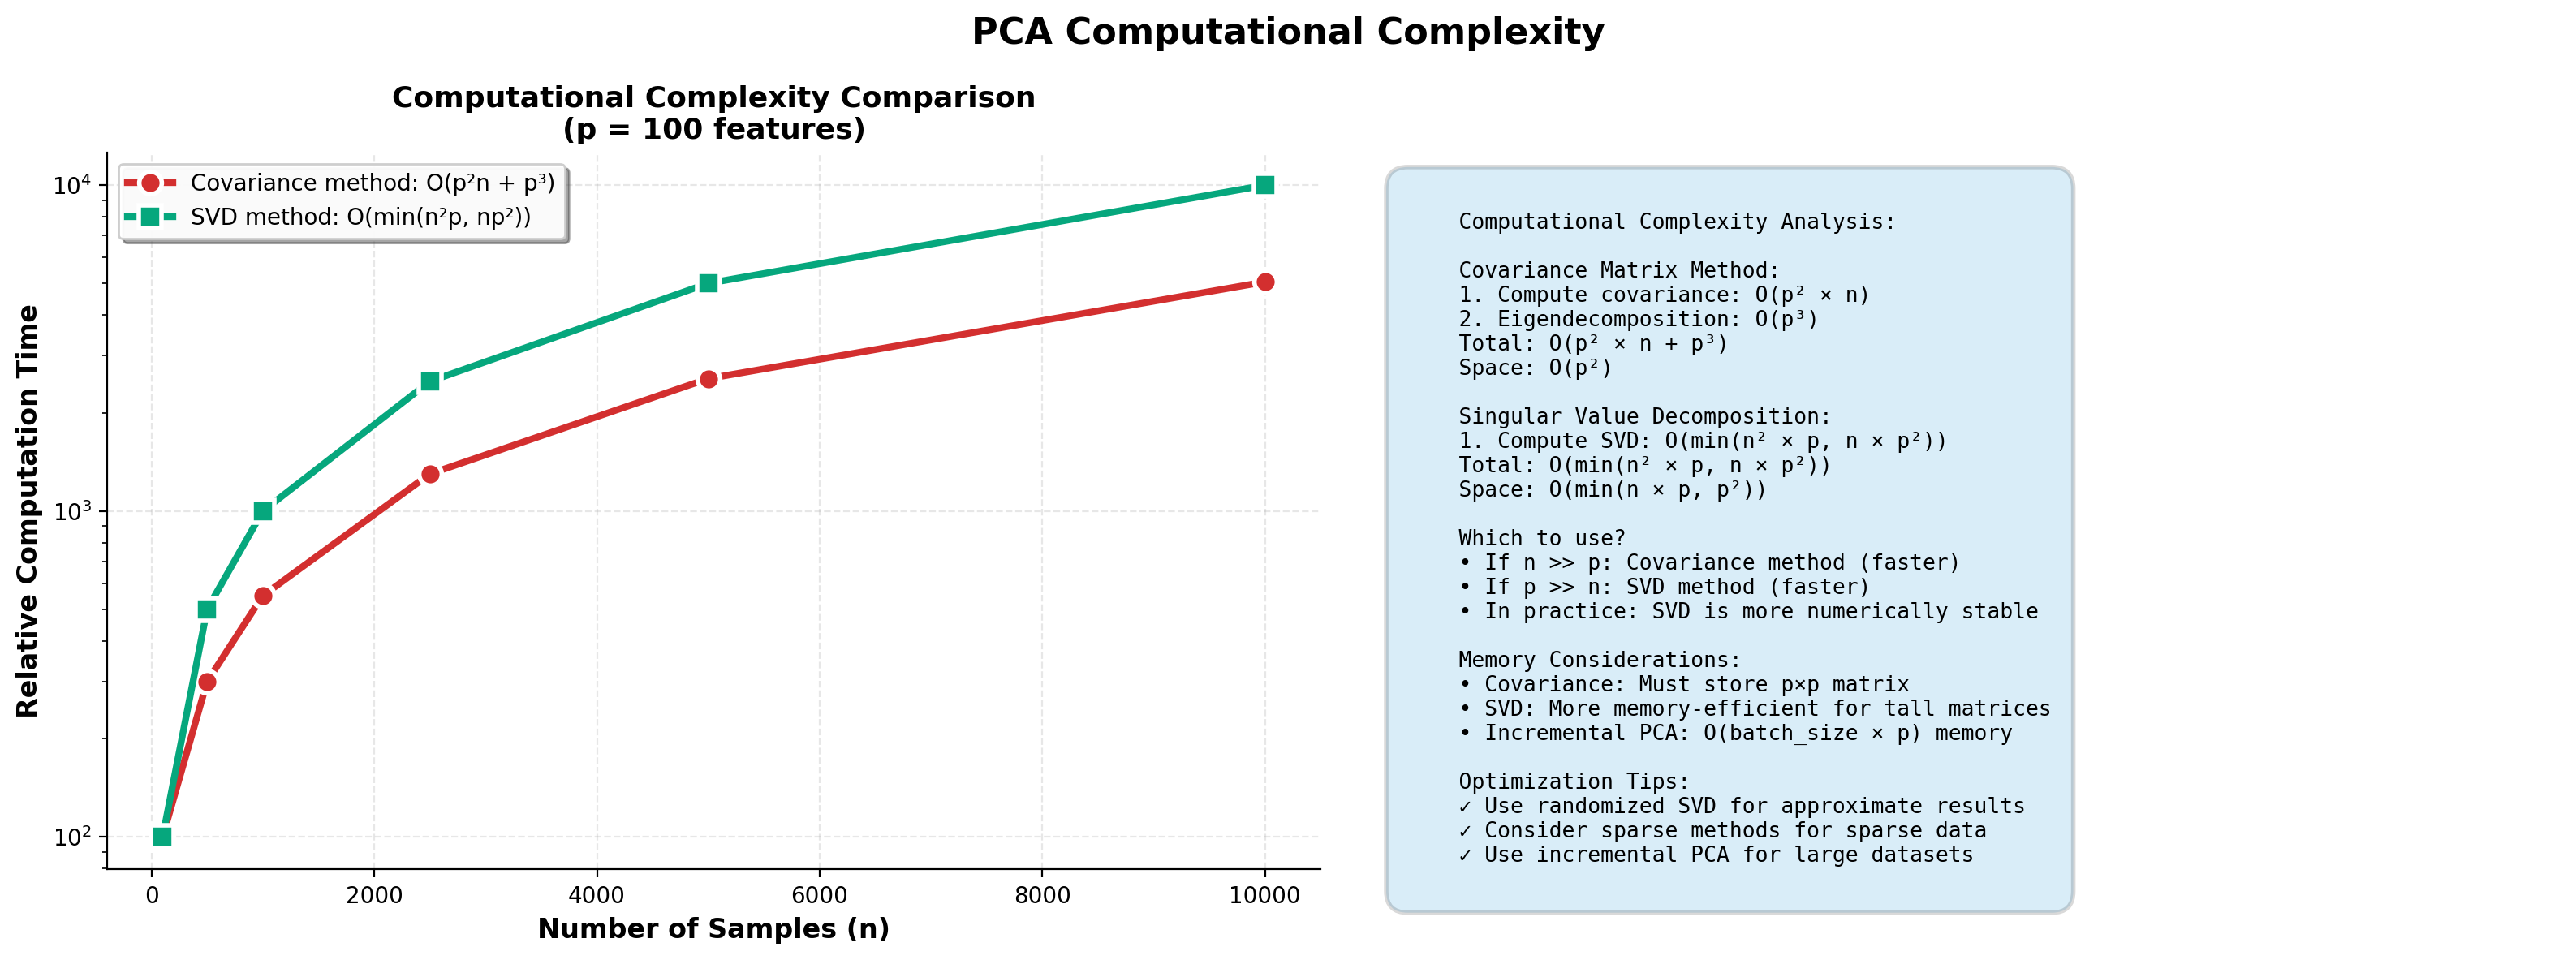
\includegraphics[width=\textwidth]{../figures/computational_complexity.png}

\vspace{0.2cm}

\textbf{Solutions for Large-Scale:}

\vspace{0.1cm}

\begin{exampleblock}{Incremental PCA}
\begin{itemize}
\setlength{\itemsep}{0pt}
\item Process mini-batches
\item Memory: $\mathcal{O}(bd + d^2)$
\item Time: $\mathcal{O}(ndk)$
\end{itemize}
\end{exampleblock}

\vspace{0.1cm}

\begin{exampleblock}{Randomized PCA}
\begin{itemize}
\setlength{\itemsep}{0pt}
\item Approximate top-$k$ PCs
\item Time: $\mathcal{O}(ndk)$
\item Much faster for $k \ll d$
\end{itemize}
\end{exampleblock}

\vspace{0.1cm}

\begin{exampleblock}{Sparse PCA}
\begin{itemize}
\setlength{\itemsep}{0pt}
\item Exploit data sparsity
\item Reduce effective dimensionality
\end{itemize}
\end{exampleblock}

\vspace{0.2cm}

\begin{alertblock}{Rule of Thumb}
Standard PCA: $n, d < 10,000$\\
Incremental: $n > 100,000$\\
Randomized: $d > 10,000$, $k \ll d$
\end{alertblock}
\end{column}
\end{columns}
\end{frame}

\begin{frame}{Common Pitfalls and How to Avoid Them}
\begin{columns}[t]
\begin{column}{0.48\textwidth}
\textbf{1. Data Leakage:}

\begin{alertblock}{Mistake}
Fitting PCA on entire dataset including test set.
\end{alertblock}

\textbf{Correct approach:}
\begin{itemize}
\setlength{\itemsep}{0pt}
\item Fit PCA only on training set
\item Transform train and test separately
\item Use same transformation for both
\end{itemize}

\vspace{0.2cm}

\textbf{2. Forgetting to Center:}

\begin{alertblock}{Mistake}
Applying PCA without centering data.
\end{alertblock}

\textbf{Why it matters:}
\begin{itemize}
\setlength{\itemsep}{0pt}
\item PCA assumes zero mean
\item Results will be incorrect
\item Always center first!
\end{itemize}

\vspace{0.2cm}

\textbf{3. Wrong Scaling Choice:}

\begin{alertblock}{Mistake}
Not standardizing when features have different scales.
\end{alertblock}

\textbf{Impact:}
\begin{itemize}
\setlength{\itemsep}{0pt}
\item PCs dominated by large-scale features
\item Misleading variance explanation
\end{itemize}
\end{column}

\begin{column}{0.48\textwidth}
\textbf{4. Interpreting PCs as Features:}

\begin{alertblock}{Mistake}
Assuming PCs have same meaning as original features.
\end{alertblock}

\textbf{Reality:}
\begin{itemize}
\setlength{\itemsep}{0pt}
\item PCs are linear combinations
\item May not have intuitive interpretation
\item Use loadings for understanding
\end{itemize}

\vspace{0.2cm}

\textbf{5. Assuming Linearity:}

\begin{alertblock}{Mistake}
Applying PCA to manifold data with non-linear structure.
\end{alertblock}

\textbf{Solution:}
\begin{itemize}
\setlength{\itemsep}{0pt}
\item Check for non-linearity first
\item Consider Kernel PCA or manifold methods
\end{itemize}

\vspace{0.2cm}

\textbf{6. Ignoring Outliers:}

\begin{alertblock}{Mistake}
Not handling outliers before PCA.
\end{alertblock}

\textbf{Impact:}
\begin{itemize}
\setlength{\itemsep}{0pt}
\item PCs skewed by outliers
\item Variance misrepresented
\item Use robust PCA if needed
\end{itemize}
\end{column}
\end{columns}
\end{frame}

\begin{frame}{Interpreting PCA Results}
\begin{columns}[t]
\begin{column}{0.48\textwidth}
\textbf{What to Report:}

\vspace{0.2cm}

\begin{enumerate}
\setlength{\itemsep}{2pt}
\item \textbf{Number of components:} $k$ chosen
\item \textbf{Explained variance:} Per component and cumulative
\item \textbf{Scree plot:} Visualize eigenvalue decay
\item \textbf{Loading matrix:} Top features per PC
\item \textbf{Biplot:} If $d$ is small
\item \textbf{Reconstruction error:} If applicable
\end{enumerate}

\vspace{0.2cm}

\textbf{Interpreting Loadings:}

\begin{itemize}
\setlength{\itemsep}{2pt}
\item Examine largest magnitude loadings
\item Group features by sign
\item Name PC based on dominant features
\item Example: "Size component", "Age component"
\end{itemize}

\vspace{0.2cm}

\begin{exampleblock}{Example}
PC1 with high loadings on [height, weight, BMI]:
\begin{itemize}
\setlength{\itemsep}{0pt}
\item Interpretation: "Body size" component
\item Positive values: Larger individuals
\item Negative values: Smaller individuals
\end{itemize}
\end{exampleblock}
\end{column}

\begin{column}{0.48\textwidth}
\textbf{Statistical Significance:}

\vspace{0.2cm}

\textbf{Bootstrap approach:}
\begin{itemize}
\setlength{\itemsep}{2pt}
\item Resample data multiple times
\item Compute PCA on each sample
\item Check stability of components
\item Report confidence intervals
\end{itemize}

\vspace{0.2cm}

\textbf{Permutation test:}
\begin{itemize}
\setlength{\itemsep}{2pt}
\item Randomly permute features
\item Compare eigenvalues to null distribution
\item Test if variance is significant
\end{itemize}

\vspace{0.2cm}

\textbf{Practical Checklist:}

\begin{itemize}
\setlength{\itemsep}{2pt}
\item $\checkmark$ Data centered/standardized?
\item $\checkmark$ Scree plot shows elbow?
\item $\checkmark$ Enough variance explained?
\item $\checkmark$ PCs interpretable?
\item $\checkmark$ No data leakage?
\item $\checkmark$ Outliers addressed?
\item $\checkmark$ Results validated?
\end{itemize}

\vspace{0.2cm}

\begin{alertblock}{Documentation}
Always document preprocessing choices and justification for $k$.
\end{alertblock}
\end{column}
\end{columns}
\end{frame}

% ========================================
% Section: Summary
% ========================================

\section{Summary}

\begin{frame}{Key Takeaways}
\begin{columns}[t]
\begin{column}{0.48\textwidth}
\textbf{Core Concepts:}

\vspace{0.2cm}

\begin{itemize}
\setlength{\itemsep}{2pt}
\item \textbf{PCA:} Linear dimensionality reduction via variance maximization
\item \textbf{Principal components:} Orthogonal directions of maximum variance
\item \textbf{Eigendecomposition:} Mathematical foundation
\item \textbf{SVD:} Practical computation method
\item \textbf{Variance explained:} Quantifies information retention
\end{itemize}

\vspace{0.2cm}

\textbf{Key Steps:}
\begin{enumerate}
\setlength{\itemsep}{0pt}
\item Center (and optionally standardize) data
\item Compute covariance or apply SVD
\item Extract eigenvectors/singular vectors
\item Project data onto top-$k$ components
\item Evaluate and interpret results
\end{enumerate}

\vspace{0.2cm}

\textbf{Variants:}
\begin{itemize}
\setlength{\itemsep}{0pt}
\item Kernel PCA: Non-linear extension
\item Sparse PCA: Interpretable loadings
\item Incremental PCA: Large-scale data
\item Robust PCA: Handle outliers
\end{itemize}
\end{column}

\begin{column}{0.48\textwidth}
\textbf{Applications:}

\vspace{0.2cm}

\begin{itemize}
\setlength{\itemsep}{2pt}
\item Data visualization and exploration
\item Image compression and processing
\item Face recognition (eigenfaces)
\item Noise filtering and denoising
\item Feature engineering for ML
\item Dimensionality reduction
\end{itemize}

\vspace{0.2cm}

\textbf{Best Practices:}
\begin{itemize}
\setlength{\itemsep}{2pt}
\item Always center data, standardize if needed
\item Use scree plot and explained variance
\item Avoid data leakage in train/test split
\item Check for outliers and non-linearity
\item Validate component selection
\item Document all preprocessing choices
\end{itemize}

\vspace{0.2cm}

\textbf{Limitations:}
\begin{itemize}
\setlength{\itemsep}{2pt}
\item Assumes linear relationships
\item Sensitive to outliers and scaling
\item Loses interpretability
\item May not preserve non-linear structure
\end{itemize}
\end{column}
\end{columns}
\end{frame}

\begin{frame}{Further Reading and Resources}
\begin{columns}[t]
\begin{column}{0.48\textwidth}
\textbf{Classic Papers:}

\vspace{0.2cm}

\begin{itemize}
\setlength{\itemsep}{2pt}
\item Pearson (1901): "On lines and planes of closest fit"
\item Hotelling (1933): "Analysis of complex statistical variables"
\item Turk \& Pentland (1991): "Eigenfaces for recognition"
\item Jolliffe (2002): "Principal Component Analysis" (book)
\end{itemize}

\vspace{0.2cm}

\textbf{Advanced Topics:}

\vspace{0.2cm}

\begin{itemize}
\setlength{\itemsep}{2pt}
\item Independent Component Analysis (ICA)
\item Non-negative Matrix Factorization (NMF)
\item t-SNE and UMAP for visualization
\item Autoencoders for non-linear PCA
\item Gaussian Process Latent Variable Models
\end{itemize}

\vspace{0.2cm}

\textbf{Software Libraries:}
\begin{itemize}
\setlength{\itemsep}{0pt}
\item \texttt{scikit-learn}: PCA, KernelPCA, IncrementalPCA
\item \texttt{numpy/scipy}: Low-level linear algebra
\item \texttt{statsmodels}: Statistical PCA
\end{itemize}
\end{column}

\begin{column}{0.48\textwidth}
\textbf{Related Methods:}

\vspace{0.2cm}

\begin{itemize}
\setlength{\itemsep}{2pt}
\item \textbf{Linear Discriminant Analysis (LDA):} Supervised dimensionality reduction
\item \textbf{Factor Analysis:} Assumes latent variables
\item \textbf{Canonical Correlation Analysis:} Multi-view learning
\item \textbf{Isomap:} Geodesic distances
\item \textbf{Locally Linear Embedding:} Manifold learning
\end{itemize}

\vspace{0.2cm}

\textbf{When to Use Alternatives:}
\begin{itemize}
\setlength{\itemsep}{2pt}
\item Non-linear structure: Kernel PCA, manifold methods
\item Labeled data: LDA, supervised methods
\item Visualization only: t-SNE, UMAP
\item Interpretability: Sparse methods, NMF
\item Very large data: Random projections, sketching
\end{itemize}

\vspace{0.2cm}

\begin{exampleblock}{Next Steps}
\begin{itemize}
\setlength{\itemsep}{0pt}
\item Practice on real datasets
\item Compare with other methods
\item Explore kernel and sparse variants
\item Study deep learning autoencoders
\end{itemize}
\end{exampleblock}
\end{column}
\end{columns}

\vspace{0.2cm}

\centering
\textbf{Thank you for your attention!}
\end{frame}

\end{document}
